\documentclass{article}

\usepackage{enumerate}
\usepackage[margin=1.5in]{geometry}
\usepackage{quiver}
\usepackage{tikzit}
\usepackage{tikz-cd}
\usepackage{amsthm}
\usepackage{amsmath}
\usepackage{amsfonts}
\usepackage{amssymb}
\usepackage{mathrsfs}  
\usepackage{braket}
\usepackage{mathtools}
\usepackage{lmodern}
\usepackage{float}



\newtheorem{theorem}{Theorem}[section]
\newtheorem{lemma}{Lemma}[section]
\newtheorem{corollary}{Corollary}[section]
\newtheorem{conjecture}{Conjecture}[section]
\newtheorem{proposition}{Proposition}[section]
\newtheorem{propositionph}{$\text{Proposition}^{ph}$}[section]

\theoremstyle{definition}
\newtheorem*{definition}{Definition}


\graphicspath{ {./images/} }
\numberwithin{figure}{section}
\setcounter{section}{-1}



\title{The Algebraic Theory\\ of \\ Topological Quantum Information}
\author{by Milo Moses}

\date{\textit{California Institute of Technology} \\ [2ex] \today}


\begin{document}


\maketitle

\newcommand{\wind}{\mathrm{wind}}
\newcommand{\Free}{\mathrm{Free}}
\newcommand{\Sym}{\mathrm{Sym}}
\newcommand{\Hom}{\mathrm{Hom}}
\newcommand{\swap}{\mathrm{swap}}
\newcommand{\id}{\mathrm{id}}
\newcommand{\SO}{\mathrm{SO}}
\newcommand{\GL}{\mathrm{GL}}
\newcommand{\End}{\mathrm{End}}

\newcommand{\RR}{\mathbb{R}}
\newcommand{\ZZ}{\mathbb{Z}}
\newcommand{\QQ}{\mathbb{Q}}
\newcommand{\CC}{\mathbb{C}}

\newcommand{\NN}{\mathcal{N}}
\newcommand{\Cc}{\mathcal{C}}
\newcommand{\C}{\mathscr{C}}
\newcommand{\LL}{\mathcal{L}}

\newcommand{\0}{\left|0\right>}
\newcommand{\1}{\left|1\right>}


\renewcommand{\P}{\textsc{\textbf{P}}}
\newcommand{\BPP}{\textsc{\textbf{BPP}}}
\newcommand{\BQP}{\textsc{\textbf{BQP}}}
\newcommand{\NP}{\textsc{\textbf{P}}}
\newcommand{\NOT}{\textsc{NOT}}
\newcommand{\CNOT}{\textsc{CNOT}}
\newcommand{\AND}{\textsc{AND}}
\newcommand{\OR}{\textsc{OR}}

\newcommand{\one}{\mathbf{1}}
\renewcommand{\Set}{\mathbf{Set}}
\renewcommand{\Vec}{\mathbf{Vec}}


\begin{abstract}
This book aims to give a comprehensive account of the algebraic theory of topological quantum information. It is intended to be accessible both to mathematicians unfamiliar with quantum mechanics and theoretical physicists unfamiliar with category theory. Additionally, this text should make a good reference for working researchers in the field. A primary focus of this text is the balancing of powerful algebraic generalities with concrete examples, principles, and applications.
\end{abstract}


\newpage

\tableofcontents

\newpage


\section{Preface}
\label{Preface}

This book is a mathematical treatment of topological quantum information, with a focus on formal algebraic aspects and a special eye towards topological quantum computation. This manuscript began as an extended set of notes from a course on topological quantum field theory given by Zhenghan Wang in the winter of 2022 at UC Santa Barbara. Through his courses, his private tutoring, and his reccomendations, Zhenghan took me from a state of almost complete ignorance of mathematical physics to being a young researcher in the field. I am greatly emdebted to him for this, and it is certain that this book would not have existed without his guidance - he richly deserves of my apple.

Great pains have been taken to make this book as pedagogical and accessable as possible. The hope is that it should be readable by both mathematicians unfamilar with quantum mechanics as well as theoretical physicists unfamiliar with category theory. A primary focus of this text is the balancing of powerful algebraic generalities with concrete examples, principles, and applications. The prerequisites for this book are a undergraduate-level understanding of topology, abstract algebra, as well as a popular-science level of familarity with quantum mechanics.

There are already many great references to learn aspects of the material covered in this book. An excellently written and relatively complete book on topological quantum information from the perspective of a physicist is Steven Simon's text \cite{simon2023topological}. Simon's book is very algebraic, but does \textit{not} include any category theory. The main references for the relevant category theory are Bakalov-Kirillov \cite{bakalov2001lectures} and Etingof-Gelaki-Nikshych-Ostrik \cite{etingof2016tensor}. While both excellent texts, they both have notable shortcomings for learning topological quantum information. Bakalov-Kirillov was written in 2001, making it very outdated. Etingof-Gelaki-Nikshych-Ostrik is modern, but makes no connections to physics and does not use the language of string diagrams. The manuscript most similar to this one is Kong-Zhang's preprint \cite{kong2022invitation}. We distinguish ourself from Kong-Zhang by our different choice of topics, our different choice of treatment, and our extended scope. Other relevant books and review articles include Wang's monograph \cite{wang2010topological}, Kauffman-Lomonaco's quantum topology themed review \cite{kauffman2009topological}, and Bartlett's topological quantum field theory PhD thesis \cite{bartlett2005categorical}.

The structure of this book is as follows.

\begin{enumerate}
\item Chapter \ref{overview} (Overview): This chapter gives an overview of the subject, and aquaints the reader with the important principles of topological quantum computation. Section \ref{conceptual introduction} gives a non-technical primer on the subject, including motivation, applications, and history. Section \ref{technical introduction} covers topological \text{classical} information, as a playing ground in which to highlight the important principles of the field. This includes a crash-course on the relevant toplogy, which may be unfamilar to some readers.

\end{enumerate}

[WORK: make it clear that this is NOT a topology textbook. The topology will be extremely handwaivy. This is an algebra textbook.]

[WORK: to add on to the above point - maybe I should add something like $\text{Theorem}^{ph}$ for ``physical theorem"? Use it only for topology stuff, never for algebra stuff.]
\newpage

\section{Overview}
\label{overview}

\subsection{Conceptual introduction}
\label{conceptual introduction}

\subsubsection{Motivation and applications}

I will take as a definition \textit{topological quantum information} to be the study of information in topological quantum systems. A topological quantum system is some mathematical or physical system which is in a fundamental sense described by the mathematics of both quantum mechanics and topology. The term \textit{quantum system} here is used in contrast to \textit{classical system}. The flow of current through a conducting copper wire is described perfectly well by classical electromagnetism, whereas the flow of current through a superconducting niobium-titanium wire necessarily requires quantum mechanics for its description.

The term \textit{topological system} is used in contrast to \textit{geometric systems}, though the term “geometric system” is a nonstandard one. In a geometric system, measurable quantities and phenomena depend on quantitative local aspects of the system - the distance between wires, the exact shape of some sample, or the curvature of some component. In a topological system, measurable quantities and phenomena depend only on qualitative global aspects of the system - whether two wires cross or not, whether a sample is connected or not, whether a component curves into a ball or has a boundary.

I say that this book is about “topological quantum information” and not “topological quantum systems” for two reasons. The first is to highlight the fact that topological quantum systems \textit{do} have local geometric descriptions, which we will mostly be ignoring them in favor of focusing on their global topological properties. The beauty of topological systems lies exactly in the fact that this global perspective retains all the essential information in the system. The second reason I use the term \textit{information} is to highlight this book’s eye towards topological quantum computing. 

Since Peter Shor’s 1994 discovery of an efficient factoring algorithm on quantum computers \cite{shor1994algorithms}, the primary goal of quantum information theorists has been to harness quantum information sufficiently well so that it can be used to make an efficient scalable quantum computer. One of the major hurdles in achieving this goal is that quantum information is \textit{fragile}. Small amounts of noise coming from nearby electromagnetic fields or imperfections in experimental devices are often enough to affect the information being stored, resulting in \textit{errors} in the computation. In the early days of quantum computing it was not clear whether there was any way around this problem. Perhaps the inherent fragility of quantum information would make quantum computation impossible. This turned out to be false.

The beautiful observation is that errors are not nearly as catastrophic in \textit{topological} quantum systems. Errors are typically local, and by definition the information topological systems does not depend on local properties. Hence, under suitable conditions, topological systems are naturally error resistant! In the same way that invariants of topological spaces are supposed to be invariant under deformations in pure mathematics, information in topological systems is invariant under errors in mathematical physics. Hence, to solve the problem of noise all one has to do is make a \textit{topological} quantum computer! This observation was made in 1997 and is due independently to Alexei Kitaev and Michael Freedman \cite{kitaev2003fault, freedman1998p}. Since then topological quantum computing has grown and evolved, finding its way into almost every modern proposal for fault-tolerant quantum computing.

The first approach to topological quantum computing is to use a physical material, some literal condensed collection of atoms, which naturally behaves as a topological quantum system. These exist and have been studied for a long time. For instance, a two dimensional sheet of graphene behaves topologically when it is subjected to low temperatures ($\approx$5 degrees Kelvin) and large magnetic fields ($\approx$15 Teslas) \cite{bolotin2009observation}. Topological quantum materials which can be used to make scalable quantum computers require intricate experiments to operate, which has been the most prominent roadblock in this approach.

The second approach to topological quantum computing is to artificially construct a topological system within a geometric one. The function of a quantum computer, almost by definition, is to simulate quantum systems. In particular, it can simulate \textit{topological} quantum systems. Since topological systems are resistant to local errors, this means that the original computer which is simulating the topological system will itself become resistant to local noise! This works exactly as described as long as the simulation itself is local, that is, local effects in the original system correspond to local effects in the simulated system. This technique of simulating a topological system to inherit its error-resistant properties is known as \textit{topological quantum error correction}. The advantage of this approach is that it works on any hardware available. The disadvantage is that to perform useful computations one must pass through the topological quantum error correction. The additional layer adds a hefty amount of overhead, which can eat up the majority of runtime and resources. It is for this reason that \textit{efficient} topological quantum error correction is an important and active area of research.

\[\begin{tikzcd}
	& \begin{array}{c} \substack{\text{topological}\\ \text{quantum}\\\text{materials}} \end{array} \\
	\begin{array}{c} \substack{\text{topological} \\ \text{quantum} \\ \text{information}} \end{array} \\
	& \begin{array}{c} \substack{\text{topological}\\\text{quantum}\\ \text{error correction}} \end{array}
	\arrow["\begin{array}{c} \substack{\text{intrinsic}\\\text{realization}} \end{array}", from=2-1, to=1-2]
	\arrow["\begin{array}{c} \substack{\text{local}\\\text{simulation}} \end{array}"', from=2-1, to=3-2]
\end{tikzcd}\]

Of course, the above discussion presents only one motivation for topological quantum information and only one example of an application. Topological quantum materials open a whole world of potential applications, and it seems they may play an important role in the techonologies of the future \cite{ramirez2020dawn}. Some proposed applications include processing classical information using topological defects in magnetic devices (with the end goal of making high-speed low-energy transmissions) \cite{marrows2021perspective, vsmejkal2018topological}, creating highly sensitive photodetectors (with the end goal of making night-vision goggles or sensors) \cite{chan2017photocurrents}, creating technolgies with high thermoelectric effect (with the end goal of making efficient fridges or electric generators) \cite{skinner2018large}, creating highly-efficient transistors \cite{fuhrer2021proposal}, and engineering tiny electrical components \cite{viola2014hall, placke2017model}. 

This breadth of potential applications is due in part to the number of different types of topological materials which have been discovered or theorized. This includes quantized Hall states \cite{von202040}, topological insulators \cite{hasan2010colloquium}, fractional Chern insulators \cite{regnault2011fractional}, Weyl/Dirac semimetals \cite{armitage2018weyl}, and topological superconductors \cite{sato2017topological}. The contents of this book certainly do not provide the entire picture for any of these materials. However, the hope is that it gives a picture of the algebraic structures within them, hence helping readers think both concretely and conceptually about these materials and their applications.

\subsubsection{Mathematical picture}

The term \textit{topological quantum system} is broad. To get a rigorous mathematical subject, we will focus on a specific type of topological quantum system known as a \textit{topologically ordered} quantum system. Topological order is much more precise, though there are still conflicting definitions in the literature. Specifically, I will be focusing on \textit{(2+1)-dimensional} topological order. Here, I am using the physicist convention of using (2+1)D to refer to two space dimensions and one time dimension. That is, I will be discussing a locally flat topologically ordered system. For example, a single sheet of graphene at low temperatures and large magnetic fields can exhibit a form of (2+1)D topological order, and any quantum computer running topological quantum error correction can also exhibits a form of (2+1)D topological order.

\begin{center}
\fbox{All systems in this book are two-dimensional unless stated otherwise.}
\end{center}

The naive mathematical description of topological order is \textit{topological quantum field theory}. In a sense, we can \textit{define} a topologically ordered system to be a system which admits a description in terms of topological quantum field theory. Geometric quantum systems require non-topological quantum field theory to describe.

While they are useful in many contexts, topological quantum field theories do have several difficulties associated with them. The most prominent of which is that their definition requires a large amount of essentially redundant data. This makes them hard to construct, inaccessible to computational methods, and opaque in their realizations of important phenomena. One solution to this problem is to dig down to the core algebraic data lying within topological quantum field theories. This algebraic data contains far less redundancy than the original topological quantum field theory. This makes the algebraic data thus easier to construct, more accessible to computational methods, and more clear in its realization of important phenomena. The algebraic structure which houses the algebraic data of a (2+1)D topological quantum field theory is known as a \textit{modular tensor category}. These algebraic structures are the main mathematical object of this text, and it is because of this focus that this book is called the \textit{algebraic theory} of topological quantum information. Once one has a modular tensor category it is easy to manipulate the stored information to perform computations. This gives us the overall schema of our mathematical discussion, as illustrated visually below:

This schema is part of a more general pattern in the field of topological mathematical physics, illustrated below:

\begin{equation*}
\tikzfig{mathematical-outline-simplified}
\end{equation*}

In Chapter [ref] we describe topological order. In Chapter [ref] we will axiomatize topological order in terms of topological quantum field theory. In Chapter [ref] we will construct the theory of modular tensor categories. In Chapter [ref] we will use the tools we have established to detail several algorithms and procedures for topological quantum computaiton. To conclude, in chapter [ref] we describe further structures in topologically ordered systems which lie beyond plain modular tensor categories. Two introductory chapters are also included: Chapter [ref] which establishes the basic theory of finite dimensional quantum systems and Chapter [ref] which establishes basic category theory.

[WORK: I removed TQFTs from the book. The mathematical outline needs to change, and comments about this outline need to change throughout the rest of the book.]

\subsubsection{History of the subject}

Like with any sufficiently rich subject, the history of topological quantum information can be traced back as far as one wants. So let me do exactly that. The first use of topology in information science was roughly 2600 BCE, with the South American \textit{Quipu} \cite{ascher1981code}. Quipu are intricate knotted strings typically made out of cotton fibers. The knots in the string are used to store various types of information, typically numbers. The Quipu store their information in knot invariants, and hence hold \textit{topological} information.

Quipu were so successful that they remained the primary method of information processing in much of South America for thousands of years. They reached their peak of usage in the 15th century via the Inca empire. The Inca empire was the largest pre-Columbian empire in the western hemisphere, with over ten million subjects and spanning over two million square kilometers. Despite their intricate government, the Incas had \textit{no written language}. This distinguished them from their contemporary empires, such as the Mali, Mongolian, or Chinese empires, which all relied on the written word. The success of the Inca empire can be seen as a testament to the versatility and power of knot invariants. The difference between the Inca and modern proposals for topological quantum computers is that instead of the strings being made out of cotton fibers they are made out of the spacetime trajectories of quasiparticles in topological systems.

Similarly, the history of topological methods in quantum mechanics can be traced back to the origins of quantum mechanics. There is a 1931 paper of Paul Dirac \cite{dirac1931quantised} which introduces many of the ideas which would become foundational to topological quantum mechanics. In the 1950s, explicitly topological ideas such as the Aharanov-Bohm effect \cite{aharonov1959significance} and the theory of point defects by Tony Skyrme \cite{skyrme1962unified} were beginning to emerge. In the 1970s nontrivial abstract topological considerations were leading to novel contributions to contemporary physics, such as the theoretical description of the A-phase of superfluid Helium-3 \cite{anderson1977phase} and the theory of phase transitions in the xy model proposed by Kosterlitz-Thouless \cite{kosterlitz1973ordering}. These results were associated with the 1996 and 2016 Nobel prize respectively.

It was in the 1980s, however, that topology established itself as one of the leading themes in condensed matter physics. The discovery of the quantum Hall effect in 1980 \cite{klitzing1980new} and the subsequent discovery of the fractional quantum Hall effect in 1982 \cite{tsui1982two} gave the first examples of topologically ordered systems in our modern sense of the word, and resulted in the 1985 and 1998 Nobel prizes respectively. These systems, along with their nontrivial algebraic descriptions, gave theorists the license to dream big about what possibilities could lie ahead. This led to major work by theorists such as Frank Wilczek \cite{wilczek1982quantum, arovas1985statistical}, Duncan Haldane \cite{haldane1983nonlinear, haldane1988model}, and others.

The most notable of these theorists for our present story is Edward Witten, with his introduction of \textit{topological quantum field theory} in 1988 \cite{witten1988topological}. This work not only put the modern experiments within a larger context, but it also connected these developments to a parallel story which had been developing within pure mathematics. Namely, knot theory. In 1984 Vaughn Jones discovered his landmark knot invariant, which was powerful in its ability to distinguish between non-equivalent knots \cite{jones1997polynomial}. This marked the first major progress in the field since Alexander's invariant in 1928 \cite{alexander1928topological}. However, Jones’ construction was steeped in opaque subfactor theory, so much so that the fact that it resulted in knot invariant felt almost like a happy accident. Hence, a widespread topic on the mind of contemporary mathematicians was how to properly interpret the Jones invariant, and how to construct other invariants like it. Witten seemed to answer both. After defining topological quantum field theory, he showed how the Jones invariant could be obtained as an observable quantity within a certain theory \cite{witten1989quantum}! This shocking result gave a new interpretation of the Jones invariant in terms of mathematical physics which was appealing to experts. Seeing as the Jones invariant was constructed from a topological quantum field theory, it was natural to expect that other theories might give new invariants which could distinguish between even more knots. This vision of invariants in low-dimensional topology constructed using topological quantum field theory became known as \textit{quantum topology}, and evolved into its own discipline in the following years.

This brings us to 1997. Quantum topology is a well developed area in pure mathematics, and topological themes in condensed matter physics are at the forefront of the field. The open problem is how to construct a fault tolerant quantum computer. Peter Shor had recently discovered his factoring algorithm \cite{shor1994algorithms}, and there was debate about whether scalable quantum error correction was possible \cite{landauer1995quantum}. This led to two independent proposals for topological quantum computation in the same year. One was by the mathematician Michael Freedman \cite{freedman1998p}. His vision was clear. A recent paper had shown that computing the Jones invariant of knots was in general an NP-hard problem \cite{jaeger1990computational}. However, by the work of Witten, the Jones invariants of knots were observables in certain topological quantum field theories. Hence, if one could construct physically a topologically ordered system which was described by Witten’s topological quantum field theory then the Jones polynomial of knots could be computed efficiently by making measurements on the system. Hence, one would obtain a very powerful computer. This was Freedman’s proposal.

The other proposal was made by theoretical physicist Alexei Kitaev \cite{kitaev2003fault}. His proposal was much more precise. He gave a toy model for a certain family of topologically ordered systems. He then outlined a technique for storing and manipulating information within these systems. The powerful observation was that every quantum algorithm could be performed using the technique he had outlined \cite{mochon2003anyons}.

In the subsequent years Freedman and Kitaev teamed up with collaborators Zhenghan Wang, Michael Larsen, and others to study the new field of topological quantum information and the possibility of constructing a topological quantum computer. One of the first major results was that no topological quantum computer could be more powerful than a standard quantum computer \cite{freedman2002simulation}. This went against Freedman’s original hope to solve NP-hard problems using topological quantum computers. Freedman’s mistake was in asserting that topological quantum computers could compute the Jones polynomial. The nmeasurements which give the Jones invariant in topological quantum field theory will always be \textit{approximate}. Approximating the Jones invariant in this way is strictly computationally easier than evaluating the Jones invariant exactly. In fact, this way of approximating the Jones invariant is \textit{not} NP-hard - it can only be used to solve problems which could efficiently be solved using standard quantum computers.

The second major result of Freedman, Kitaev, Wang, and Larsen was the converse of their first result \cite{freedman2002modular}. Namely, they showed that every quantum algorithm can be efficiently run on a topological quantum computer. They do this by showing that every quantum algorithm can be efficiently reinterpreted in terms of computing the Jones invariant of some knot. In this way, computing the Jones invariant is a \textit{universal problem} for quantum computation. They then formalize Freedman’s ideas about topological quantum field theory, and show directly that realistic operations on a topologically ordered quantum system described by Witten’s quantum field theory can be used to compute the Jones invariants of knots.

Together, these two results show that in a real sense topological quantum computing is equally powerful as standard quantum computing with quantum circuits. This laid the groundwork for fruitful studies of fault-tolerant topological quantum computing, both using error correcting codes and physical materials. This has resulted in a great number of important results, which we will discuss at length throughout the rest of this manuscript.

\subsection{Technical introduction}
\label{technical introduction}

\subsubsection{Principles of topological quantum information}

In this section I will lay out the general principles of topological quantum information. As an organizational tool, I will introduce these principles one by one as I construct a sample topological system. This example is meant to be representative of the systems we will encounter throughout this text, and within the broader field of topological quantum information. As a further organization tool, I will construct this example with the stated goal of obtaining a topological quantum computer.

Our system will be flat, containing only \textit{two spatial dimensions}. Our system will be mostly homogenous, essentially identical everywhere, at the exception of finitely many localized regions. These regions will differ substantially from the top-dimensional homogeneous bulk. These localized regions are called \textit{quasiparticles}. The beauty of systems like these is that they behave as though homogeneous bulk were empty, and the quasiparticles were fundamental particles within the bulk. In fact, in its algebraic description, these topological systems are \textit{identical} to ones in which the homogenous bulk is empty and the quasiparticles are fundamental particles. This is where the term quasiparticle arises. It is important however to remember that in most relevant applications the bulk is \textit{not} empty and the quasiparticles are \textit{not} fundamental particles. The bulk will typically be some highly entangled wavefunction, and the quasiparticles will be emergent phenomena made up of smaller microscopic degrees of freedom.

\begin{figure}[h]
\begin{center}
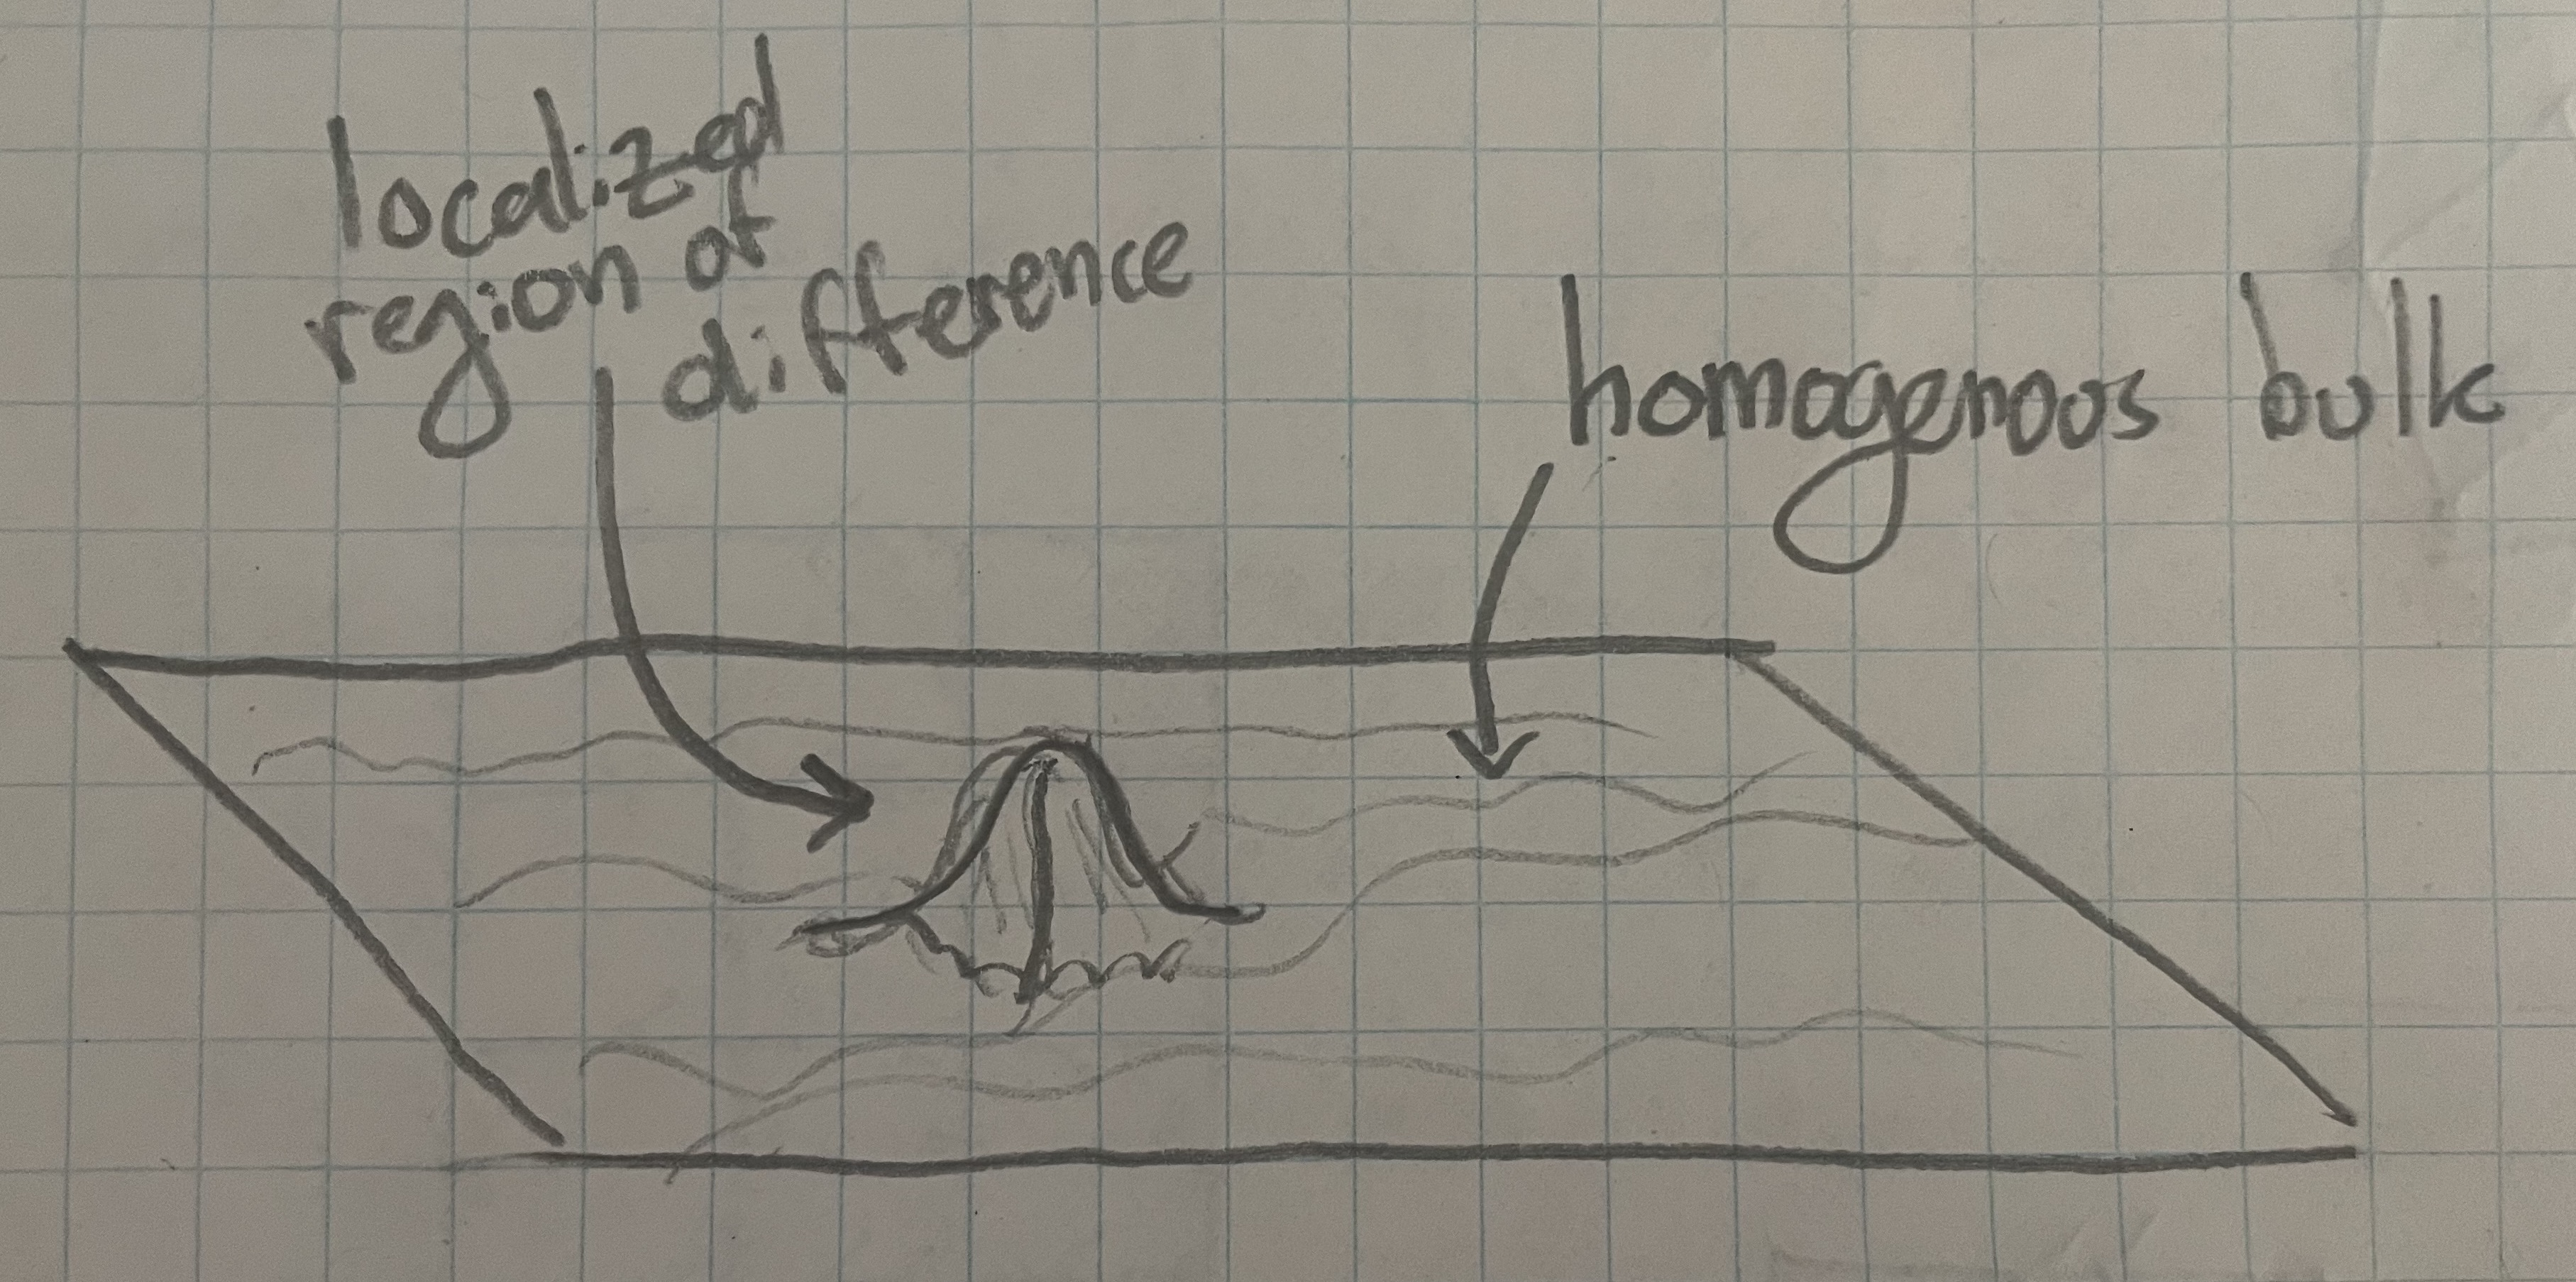
\includegraphics[scale=.04]{quasiparticle}
\end{center}
\end{figure}

Our aim is to build a computer. In general this requires three components:

\begin{enumerate}
\item A method of storing information;
\item A method of manipulating information;
\item A method of reading out information.
\end{enumerate}

Information is stored in the state of the system - the bulk is described by some parameters, and the details of those parameters encodes information. Our method for manipulating information is \textit{braiding}. Braiding is the process whereby quasiparticles are moved along continuous paths around one another. There are two important points about braiding to keep in mind. The first is that braiding changes the state of the system. Even though the quasiparticle content of the system may be identical before and after the braid, the details of the system will change - there is more to the state of the system than just the positions of the quasiparticles. The second point is that the way that the state of the system changes depends \textit{only depends on the topology of the braid}, and not the geometry. Small deformations in the path taken by the quasiparticles do not affect the result - only global changes, like whether a path is taken clockwise or counterclockwise, makes a difference. This invariance is due to the fact that our system is topological. In geometric systems we expect the exact path taken by quasiparticles matters a great deal. The independence of the details of the paths is extremely specific to topological systems, and in the present setting is the \textit{defining topological feature}.

It is at this point that we can already see we have succeeded in our goal of making our computations fault-tolerant. Noise in the system will correspond to uncontrolled perturbations in the trajectories of the quasiparticles. This uncontrolled movement won’t change global properties of paths taken, and hence will not change the action of the braids on the system. That is, small errors will not affect computation! Of course, large enough errors could unintentionally make one quasiparticle wind around another. This would change the topology of the braid and hence ruin the computation. These errors are controllable, however, by moving the quasiparticles far apart and limiting the magnitude of the noise.

The final step in making our computer is to introduce a method for reading out information. This is done using \textit{fusion}. Fusion is the process whereby two quasiparticles are brought together, resulting in a single quasiparticle. In sufficiently complicated topological systems the result of fusion depends on the details of the state of the overall system. That is, the result of fusion can be used as a way of reading out information about the state. In its most basic form, when two quasiparticles fuse they can either result in a localized region which is identical to the homogenous bulk or is different from the homogenous bulk. If they result in a localized region identical to the bulk we say that the two quasiparticles have \textit{annihilated} each other. In a real sense this can be seen as the difference between constructive and destructive interference. Two waves can either have destructive interference and annihilate each other, or they can constructively interfere and result a new wave. Measuring whether or not two quasiparticles annihilate upon fusion gives a method for reading out information.

In some situations, the result of fusion can even be nondeterministic. In this case the fusion can be repeated multiple times, which allows one to measure the \textit{probability} that two quasiparticles will annihilate each other. These probabilities are a rich source of data, and will serve as our way of reading out information in the current setting. The fact that our system is topological implies that the result of fusion does not depend on the specifics of the path taken, and hence this method of readout preserves the invariance of our computation to noise. This gives us a full picture of topological quantum computation, as seen in figure \ref{fig:TQC-outline}.

\begin{figure}
\begin{center}
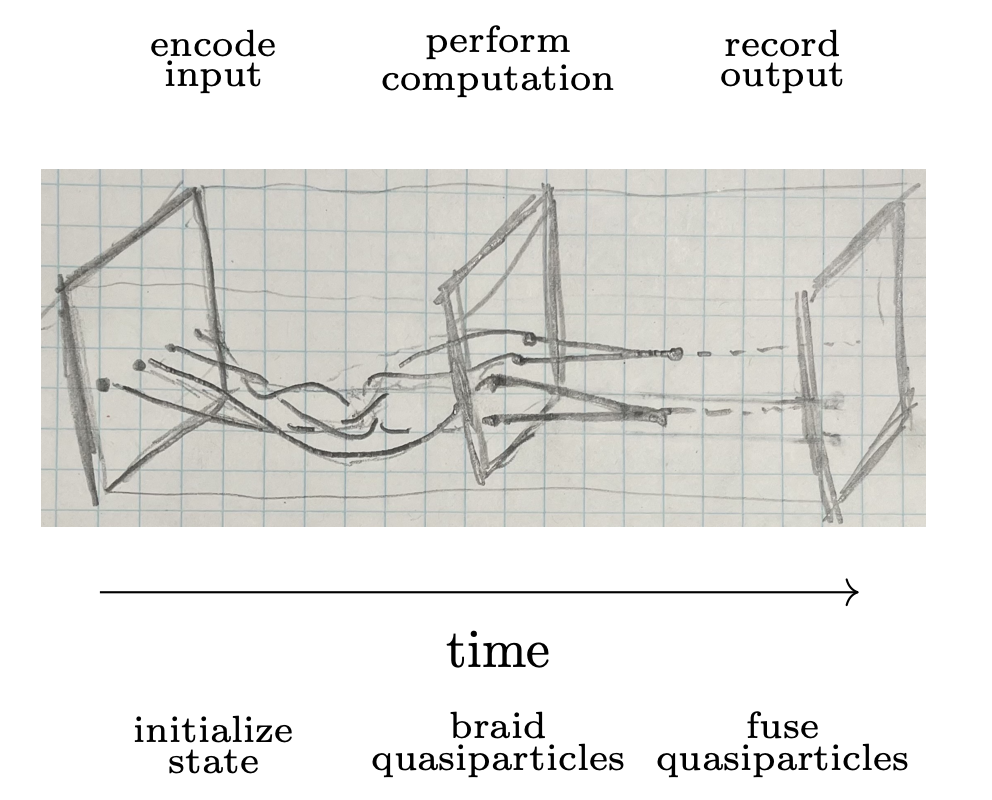
\includegraphics[scale=0.35]{TQC-outline}
\caption{A schematic of topological quantum computing}
\label{fig:TQC-outline}
\end{center}
\end{figure}

To make the above discussion more concrete, we will give a worked example. In this example we use a specific topological order known as the \textit{Fibonacci particle theory} to run Shor’s efficient quantum factorization algorithm \cite{shor1994algorithms}. The input of Shor’s algorithm is a positive integer. The output of Shor’s algorithm is the factorization of that integer. Shor’s algorithm is \textit{efficient} in the sense that it uses polynomially many quantum logic gates to arrive at its answer relative to the size of the input. Throughout this passage we will use \textit{efficient} and \textit{polynomially sized} interchangeably. The Fibonacci particle theory is a specific topological order, which describes in an algebraic fashion how the overall state changes when quasiparticles are braided and fused.

The first step in running Shor’s algorithm on a Fibonacci quantum computer is to translate the positive integer input into a certain braid. This is done using an efficient classical algorithm. The second step is to run this braid on a Fibonacci quantum computer. This is done by initializing some prescribed state and then braiding its quasiparticles. This initialization and braiding is performed repeatedly, and after every time two of the quasiparticles are fused. This gives us a real number, which is the probability that the two quasiparticles annihilate after the braiding. An efficient classical algorithm is then used to take this real number and obtain from it the factorization of the original input. Since all of these steps are efficient, it gives a topological quantum algorithm for factoring integers. The schematic for this process is shown below:

\begin{equation*}
\tikzfig{shor-fibonacci}
\end{equation*}

The magic in the above procedure is the existence of these two classical algorithms: a first one for encoding integers into braids and a second one for decoding real numbers into factorizations. These algorithms are nontrivial. They are due to Freedman-Larsen-Kitaev-Wang \cite{freedman2002modular}. In fact, Freedman-Larsen-Kitaev-Wang showed that any problem which can be efficiently solved using a quantum circuit can also be solved using the Fibonacci particle theory, via a similar method of efficient classical preprocessing and postprocessing. It is in this sense that the Fibonacci theory is \textit{universal} for quantum computation.

The final step of this process would be to create a physical topological system which is described by the Fibonacci theory, which would serve as our quantum computer. In the realm of materials, the most promising approach seems to be to use specially tuned versions of the fractional quantum Hall system \cite{zhu2015fractional}. While these materials are theorized to host quasiparticles described by the Fibonacci theory, the difficulty of the experiment makes them inaccessible to current technology. There has been progress made on topological quantum error correcting codes which work by simulating the Fibonacci theory \cite{schotte2022quantum, schotte2022fault}. However these codes at the current moment have structural issues and require an unbearable amount of overhead to run, making them unfeasible to use on modern computers.

Progress on topological quantum computing has thus been focused on realizing topological particle theories other than the Fibonacci theory. These other theories can be constructed in more workable materials, and can be simulated as topological quantum error correcting codes with less overhead. The drawback of these other theories is that they are typically less computationally powerful, meaning that they require more tricks and techniques to achieve universal quantum computing. There are a great number of different proposals for how to achieve universal topological quantum computing, based on different particle theories, different methods of encoding information, different methods of manipulating information, and different methods of reading out information. It is an exciting time to be a theorist in the field of topological quantum information.

\subsubsection{Defects in ordered media}

We will now work through a complete mathematical example of a family of topological systems. Our examples will be \textit{classical} topological systems. Many of the important subtlties of topological quantum information are already present in the classical case. Topological classical information is a smaller subject than topological quantum information - the reader should have a relatively complete grasp of the subject by the end of the chapter. Much of the discussion in this chapter is taken from an excellent review article by Mermin \cite{mermin1979topological}. The goal of this chapter is both to give a family of relevant examples to the reader, as well as to give a crash-course on the relevant topology.

The family of systems we will describe goes by many names. In communities of experimentally focused physicists it goes by the name \textit{ordered media}. In mathematical physics communities it goes by the name \textit{classical gauge theory} [WORK: is ``classical gauge theory" really a thing, or is this ``classical field theory"? I should ask a physicist to make sure I've got my terminology right.]. In pure mathematics it would be described as \textit{homotopy theory}. We will construct a system based on every topological space $M$. We will call $M$ the order space of our theory.

To describe a system in physics, the first step is to define the space of possible states of the system. In this case, states will correspond to \textit{continuous maps $\phi: \RR^2\to M$}. We now give physical intuition for this choice of state space. The choice of $\RR^2$ as a source represents the underlying material. We are working on an infinite flat plane. Describing a function $\phi: \RR^2\to M$ amounts to choosing a value $\phi(x)$ for every point $x\in \RR^2$. In this way we imagine our system as being made up of infinitely many objects, one placed at each point in $\RR^2$, each of which has an internal state space $M$. The fact that $\phi$ must be continuous is a compatibility condition between the states of the objects at nearby points. It says that nearby objects must have similar states. We now list some examples:

\begin{itemize}
\item \textbf{Classical XY model of a 2D electron gas}. In this example, $M$ is the circle. An electron can be modeled as a point particle with a magnetic dipole pointing in some direction. This magnetic dipole is known as the \textit{spin} of the election, and can point in any direction in the plane. The topological space of all possible directions in the plane is a circle. The fact that nearby electrons must have similar spins is known as Hund’s rule, and is the most fundamental incarnation of ferromagnetism. It is physically derived as a consequence of the Pauli exclusion principle.

\item \textbf{A-phase of superfluid Helium-3}.  [WORK: fill in example]

\item \textbf{Biaxial nematics}. In this example, $M$ is a certain quotient of the special orthogonal group $\SO(3)$ of rotations in three dimensional space. The objects at every point in the biaxial nematic should be thought of as small rectangles with unequal side lengths. These rectangles can be oriented in any direction in three dimensional space. In practice these objects will often be molecular compounds. They will not be exactly rectangular, but have the same symmetry group as a rectangle which is enough for the model to be accurate. To compute the space of possible orientations of a small rectangle, we work by the method of symmetries. Choosing some reference orientation to start with, every rotation in three dimensional space brings the rectangles to new orientations. The space of orientations of the rectangle is hence equal to $\SO(3)$ modulo the rotations which fix the rectangle. That is, $M$ is equal to $\SO(3)$ modulo the symmetry group of a rectangle. [WORK: Talk to someone who knows about biaxial nematics. What's with the continuity condition? How does this work, really?]
\end{itemize}

We will now analyze these systems. In doing this analysis we will want to use the ideas of \textit{deformation} and \textit{topological equivalence}. Of course, these ideas are vague and require rigorous notions to make precise. We define these notions now.

\begin{definition}
Let $X,Y$ be topological spaces, and let $f,g: X\to Y$ be continuous maps. A \textbf{homotopy} between $f$ and $g$ is a map $H: X\times [0,1] \to Y$ such that $H(x, 0)=f(x)$ and $H(x,1)=g(x)$ for all $x\in X$.
\end{definition}

The idea is that the maps $H(\cdot,t):X\to $Y for $t\in [0,1]$ are a continuously deforming family. The first map $H(\cdot, 0)$ is equal to $f$, and as $t$ moves forward the maps $H(\cdot,t)$ slowly change until at $t=1$ they become $H(\cdot,1)=g$. If there exists a homotopy between two maps, then we say those maps are \textit{homotopic}. It is straightforward to verify that homotopy is an equivalence relation (see Exercise [ref]). More colloquially, if $f$ and $g$ are homotopic we say that $f$ can be deformed into $g$. This is our relevant notation of topological equivalence.

We can use homotopies to get a picture of dynamics in our system. We call continuous maps $H: \RR^2 \times \RR_{\geq 0}\to M$ \textit{time evolutions} of the system. The map $\phi_t=H(\cdot,t): \RR^2\to M$ is called \textit{the state of the system at time $t$}. For every $T>0$, the map $H_T:\RR^2\times [0,1]\to M$ given by $H_T(x,t)=H(x,t\cdot T)$ gives a homotopy between $\phi_0$ and $\phi_T$. Hence, the states of the system at various times are all homotopic. In this sense the system is \textit{evolving by homotopies}. The following proposition is an important part of understanding the nature of the system:

\begin{proposition}
Let $M$ be a path connected topological space. Every pair of continuous maps $\phi_0,\phi_1:\RR^2\to M$ is homotopic.
\end{proposition}
\begin{proof}
Consider the map $H_0: \RR^2\times [0,1]\to M$ given by $H_0(x,t)=\phi_0(tx)$. Since multiplication in $\RR^2$ is continuous, $H_0$ is continuous. Hence, $H_0$ gives a homotopy between the constant map $H_0(\cdot,0)=\phi_0(0)$ and $H_0(\cdot,1)=\phi_0(x)$. Similarly, the map $H_1:\RR^2\times [0,1]\to M$  given by $H_1(x,t)=\phi_1(tx)$ gives a homotopy between the constant map $H_1(\cdot,0)=\phi_1(0)$ and $H_1(\cdot,1)=\phi_1(x)$.

Now, since $M$ is path connected, there exists a continuous map $\ell: [0,1]\to M$ such that $\ell(0)=\phi_0(0)$ and $\ell(1)=\phi_1(0)$. Thus, the map $H_\ell:\RR^2\times [0,1]\to M$ given by $H_\ell(x,t)=\ell(t)$ establishes a homotopy between the constant maps $H_\ell(\cdot,0)=\phi_0(0)$ and $H_\ell(\cdot,1)=\phi_1(0)$. Composing the homotopies from $\phi_0(x)$ to $\phi_0(0)$, $\phi_0(0)$ to $\phi_1(0)$, and $\phi_1(0)$ to $\phi_1(x)$, we arrive at a homotopy between $\phi_0(x)$ and $\phi_1(x)$ as desired.
\end{proof}

The above proposition can be interpreted as saying that as our system evolves in time, we can expect it to go from any state to any other state. In other words, all of the possible states of our system are topologically equivalent and hence it contains \textit{no topologically invariant information}. This means that we will need to add more complexity to the system before we can study topological information.

This complexity will come from introducing quasiparticles. These quasiparticles go by many names. In the theory of ordered media they are known as defects. In gauge theory they are known as particles. In homotopy theory they are known as point singularities. For the sake of brevity, we will use the term defect. A defect is a point at which we will drop our condition that the state $\phi:\RR^2\to M$ be continuous. This is done by making $\phi$ \textit{undefined} at certain points. Our new system is called \textit{ordered media with finitely many defects}. The state space consists of pairs $(S,\phi)$, where $S\subset \RR^2$ is a finite set and $\phi: \RR^2\\ S\to M$ is a continuous map.

Dynamics in our new system can involve the movement of defects. Let $\gamma_1… \gamma_n: \RR_{\geq 0} \to \RR^2$ be continuous maps, with $ \gamma_i(t)\neq \gamma_j(t)$ for all $i\neq j$, $t\in [0,1]$. These maps represent the trajectories of the defects, subject to the condition that no two defects collide. Continuous maps

$$H:\RR^2\times \RR_{\geq 0} \backslash \bigcup_{t\geq 0}\bigcup_{i=1}^{n}(\gamma_i(t),t)\to M$$

represent dynamics in our system. We call such maps \textit{defect-mobile homotopies}. At every time $t\geq 0$, the system is in the $n$-defect state

$$\phi_t=H(\cdot,t): \RR^2\backslash \bigcup_{i=1}^{n}\gamma_i(t)\to M.$$

. If the trajectories $\gamma_i$ are constant with respect to $t$ for all $i$, we will call $H$ a \textit{defect-fixed homotopy}. This now leads us to two immediate questions:

\begin{enumerate}
\item What information is invariant under defect-mobie homotopy?
\item What information is invariant under defect-fixed homotopy?
\end{enumerate}

After answering these questions, we will move on to building a computer based on defects in ordered media. The idea is that our computer will store its information within attributes of the state which are invariant under defect-fixed homotopy. These attributes, typically, will \textit{not} be invariant under defect-mobile homotopy. This means that if defects are braided around eaech other, the values of these defect-fixed attributes will change. This change in information is a \textit{computation}. This leads to two more central questions:

\begin{enumerate}
\setcounter{enumi}{2}
\item How does braiding affect defect-fixed information?
\item Which choices of order  space $M$ make for effective computers?
\end{enumerate}

Answering these questions requires a detailed analyis of our model using techniques from homotopy theory.

\subsubsection{The fundamental group}

In this subsection we analyse defects in ordered media using the \textit{fundamental group} from homotopy theory. Readers familiar with homotopy theory should familiarize themselves with the statement of Proposition [ref] before moving on to the next subsection. We begin with some terminology and basic results - we will return to ordered media breifly.

\begin{definition} Let $X$ be a topological space.
\begin{itemize}
\item A continuous map $\gamma:[0,1]\to X$ is called a \textbf{path} in $X$ from $\gamma(0)$ to $\gamma(1)$;
\item Given two paths $\gamma_0,\gamma_1$ with the same start and end points, a \textbf{path homotopy} from $\gamma_0$ to $\gamma_1$ is a map $H:[0,1]\times [0,1]\to X$ such that $H(\cdot,0)=\gamma_0$, $H(\cdot,1)=\gamma_1$, $H(0,t)=\gamma_0(0)=\gamma_1(0)$, and $H(1,t)=\gamma_0(1)=\gamma_1(1)$ for all $t\in [0,1]$.
\item A \textbf{loop} is a path with the same start and end point. This common start and end point is called the \textbf{base point} of the loop.
\item Given a point $x\in X$, the \textbf{fundamental group of $X$ based at $x$} is defined as a set to be the collection of equivalence classes of loops in $X$ based at $x$ up to path homotopy. It is denoted $\pi_1(X,x)$.
\end{itemize}
\end{definition}

The term fundamental \textit{group} is justified by the following proposition:

\begin{proposition} Let $X$ be a topological space, and let $x\in X$ be a point. We define a binary operation on the space of loops in $X$ based at $x$ by the formula 

$$(\alpha_0\cdot \alpha_1)(t)=
\begin{cases}
\alpha_0(2t) & 0\leq t < 1/2\\
\alpha_1(2t-1) & 1/2\leq t \leq 1
\end{cases}$$

for all loops $\alpha_0,\alpha_1$ based at $x$. This binary operation induces a well-defined map path homotopy equivalence classes, yielding a binary operation on $\pi_1(X,x)$. This binary operation endows $\pi_1(X,x)$ with the structure of a group.
\end{proposition}
\begin{proof}.[WORK: do proof]
\end{proof}

We now prove some basic results about the fundamental group:

\begin{proposition} Let $X$ be a topological space, and let $x\in X$ be a point.
\begin{enumerate}[(a)]
\item Let $\gamma:[0,1]\to X$ be a path. Given every loop $\alpha$ in $X$ based at $\gamma(0)$, define the map

$$i_\gamma(\alpha)(t)=
\begin{cases}
\gamma(1-3t) & 0\leq t < 1/3 \\
\alpha(3t-1) & 1/3 \leq t <2/3 \\
\gamma(3t-2) & 2/3 \leq t \leq 1
\end{cases}$$

to be a loop based at $\gamma(1)$. This assignment induces a well defined map on path homotopy equivalence classes. Moreover, the induced map

\begin{equation*}
i_\gamma: \pi_1(X,\gamma(0))\xrightarrow{}\pi_1(X,\gamma(1))
\end{equation*}

is an isomorphism of groups.

\item Let $S^1$ be the circle, which we define as the interval $[0,1]$ with $0$ and $1$ identified. Every loop in $X$ induces a map from the circle to $X$, by gluing $0$ and $1$. This natural map induces a \textbf{bijection} between conjugacy classes in the fundamental group and homotopy classes of maps from the circle to $X$.

\end{enumerate}
\end{proposition}
\begin{proof}. [WORK: do proof]
\end{proof}

The fundamental group of the order space $M$ will play an important role in our analysis of the system. Hence, we will now compute the fundamental groups of the order spaces corresponding to the xy model of an electron gas, the A-phase of superfluid helium, and biaxial nematics:

\begin{proposition}$\,$
\label{fundamental-group-computations}
\begin{enumerate}[(a)]
\item $\pi_1(S^1,x)\cong \ZZ$ for all $x\in S^1$;
\item $\pi_1(\RR^2\backslash S,x)\cong\Free(S)$ for all finite sets $S\subset \RR^2$ and $x\in \RR^2\backslash S$, where $\Free(S)$ denotes the free group with generators corresponding to elements of $S$.
\item .[WORK: compute superfluid helium example];
\item .[WORK: compure biaxial nematics example];
\item For all groups $G$, there exists a topological space $X$ such that $\pi_1(X,x)\cong G$ for all $x\in X$.
\end{enumerate}
\end{proposition}
\begin{proof}.[WORK: do proof]
\end{proof}

As a consequence of proposition \ref{fundamental-group-computations}(a), we can define the notion of \textit{winding number}.

\begin{corollary} Choose $b,x\in \RR^2$. We have a canonical isomorphism of groups $\pi_1(\RR^2\backslash \{x\},b)\cong \ZZ$. Given a loop $\alpha:[0,1]\to U\backslash \{x\}$ based at $b$, the integer corresponding to the element $[\alpha]\in \pi_1(U\backslash \{x\},b)$ is called the \textbf{winding number of $\alpha$ around $x$}. It is denoted $\wind(\alpha,x)$.
\end{corollary}
\begin{proof}.[WORK: do proof]
\end{proof}

We are now ready to return to our analysis of defects in ordered media. Let $(S,\phi)$ be a state in an ordered media with order space $M$. Suppose $S=\{x_1, ...x_n\}$, and choose a basepoint $b\in \RR^2\backslash S$. For all $1\leq i\leq n$, define loops $\alpha_i$ based at $b$ which go around $x_i$ exactly once counterclockwise, and do not wind around any of the other $x_j$. Formally, this amounts to choosing $\alpha_i$ so that

$$\wind(\alpha_i,x_j)=
\begin{cases}
1 & i=j\\
0 & \text{otherwise}.
\end{cases}$$

Each map $\alpha_i$ can be postcomposed with $\phi$ to give a map $(\phi\circ \alpha_i): [0,1]\to M$. In this way, every loop in phtsical space can be pushed forward to a loop in order space. The important feature to notice is that as $\phi$ changes by homotopies, the map $\phi\circ \alpha_i$ changes by homotopies. Additionally, as $\alpha_i$ changes by homotopies, the map $\phi\circ \alpha_i$ changes by homotopies. In this way, the homotopy class of $\phi\circ \alpha_i$ as a map from the circle to $M$ is an invariant of $\phi$ which is invariant under defect-mobile homotopy. Moreover, Proposition [ref](b) implies that all maps which wind exactly once around $\alpha_i$ and wind zero times around the other $\alpha_j$ are homotopic [WORK: this is false]. Hence, the value of the invaraint does not depend on the choice of $\alpha_i$. By Proposition [ref](b), homotopy classes of loops in order space correspond to conjugacy classes in $\pi_1(M,m)$ for any fixed $m\in M$. Hence, we conclude that associated to every defect in $\phi$, there is a corresponding conjugacy class in $\pi_1(M,m)$ for any fixed $m\in M$. This conjugacy class is an invariant under defect-mobile homotopy.

All of the path homotopy classes of maps $\phi\circ \alpha_i$ give elements of $\pi_1(M,\phi(b))$. It is natural to ask why these elements are not invariants under defect-mobile homotopies, but only their conjugacy class. The answer is twofold:

\begin{enumerate}
\item As $\phi$ changes by homotopies, $\phi(b)$ can change. This movement of basepoint will affect the path homotopy class of $\phi\circ \alpha_i$.
\item As the state changes under defect mobile homotopy, another defect $x_j$ could pass through $\alpha_i$. At this point, the composition $\phi\circ \alpha_i$ becomes \textit{undefined}. The homotopy classes of $\phi\circ \alpha_i$ before and after $x_j$ moves through it could be different. Choosing $\alpha_i$ smaller so that $x_j$ does not pass through it is possible, but this might neccecarily involve changing the basepoint of $\alpha_i$. This change in basepoint. will affect the path homotopy class of $\phi\circ \alpha_i$. [WORK: add picture]
\end{enumerate}

Under defect-fixed homotopy, the concern (2) dissapears. Moreover, if we add the technical condition that $\phi(b)$ cannot change during the defect-fixed homotopy then the concern (1) will dissapear as well. Hence, the elements $\pi_1(M,\phi(b))$ are invariants under basepoint-preserving defect-fixed homotopies. If the basepoint is allowed to vary it will change all of the path homotopy classes at once. This brings us to our main result of the subsection, which gives a full classification of information stored within defects in ordered media:

\begin{proposition} Let $M$ be a path connected topological space. Let $S=\{x_1...x_n\}$ be a finite set, and let $\phi:\RR^2 \backslash S\to M$ be a continuous map. Let $\alpha_i$ be loops in $\RR^2\backslash S$ based at $b\in \RR^2\backslash S$ such that

$$\wind(\alpha_i,x_j)=
\begin{cases}
1 & i=j\\
0 & \text{otherwise}.
\end{cases}$$

\begin{enumerate}[(a)]
\item The homotopy classes $[\phi\circ \alpha_i]$ of maps $S^1\to M$ do not depend on the choice of $\alpha_i$. These homotopy classes are invariants under defect-mobile homotopy.
\item The path homotopy classes of $[\phi\circ \alpha_i]\in \pi_1(M,\phi(b))$ do not depend on the choice of $\alpha_i$. These path homotopy classes are invariant under defect-fixed homotpies which preserve the value of $\phi(b)$. These invariants establish a bijection

$$\left(\substack{\text{states $(S,\phi)$ up to} \\ \text{basepoint-preserving defect-fixed homotopy}}\right)\xrightarrow{\sim} \prod_{i=1}^n\pi_1(M,\phi(b))$$

\item The element $\left([\phi\circ\alpha_i]\right)_{i=1}^n \in \prod_{i=1}^n\pi_1(M,\phi(b))$ does not depend on the choice of $\alpha_i$. This establishes a bijection [WORK: state this correctly - it should be simultanous conjugation by an element of $\pi_1(M,\phi(b))$]

$$\left(\substack{\text{states $(S,\phi)$ up to} \\ \text{defect-fixed homotopy}}\right)\xrightarrow{\sim} \left(\text{conjugacy classes in }\prod_{i=1}^n\pi_1(M,\phi(b))\right)$$
\end{enumerate}
\end{proposition}
\begin{proof}.[WORK: do proof]
\end{proof}

[WORK: there IS some dependence on the $\alpha_i$]

\subsubsection{Topological classical computation}

Our goal in this section is to make a topological computer. Throughout this section we will fix some notation. We let $M$ be a path connected topological space, we let $S=\{x_1, ...x_n\}$ be a finite set, we let $\phi:\RR^2\backslash S\to M$ be a state, and we let $b\in \RR^2\backslash S$, $m\in M$ be basepoints. Throughout this section we will assume that $\phi(b)=m$ is \textit{fixed}. This is mainly a matter of convenience - allowing it to move would require a tedious amount of digressions about conjugacy classes. Physically, this can be justified by pushing the basepoint away towards infinity where it cannot be disturbed.

Proposition [ref] tells us that basepoint-preserving defect-fixed homotopy classes of states correspond to elements of $\prod_{i=1}^n\pi_1(M,m)$. It is in this product that we will store our information. For example, if $\pi_1(M,m)\cong \ZZ_2$ then $\prod_{i=1}^n\pi_1(M,m)=\prod_{i=1}^n\ZZ_2$ is an $n$-bit string. More generally, one will need to outline some encoding method for converting standard information storage formats into elements of $\prod_{i=1}^n\pi_1(M,m)$.

The general picture to have in mind is that of an experimenter who has control over the trajectories of defects, but no control over the specifics of the map $\phi$ in the bulk. The goal is to engineer a protocol by which every map $f:\prod_{i=1}^n\pi_1(M,m)\to\prod_{i=1}^n\pi_1(M,m)$ can be realized by braiding defects around each other.

Let $S'=\{x_1', ...x_n'\}$ be another finite set. Let $\gamma_1..\gamma_n$ be paths in $\RR^2$ such that $\gamma_i(0)=x_i$, $\gamma_i(1)=x_i'$, $\gamma_i(t)\neq b$, and $\gamma_i(t)\neq \gamma_j(t)$ for all $i\neq j$, and $t\in [0,1]$.

As the defects in $S$ move along the paths $(\gamma_i)_{i=1}^n$, the overall state of the system will change. This will allow us to perform computations. An important feature is that the way the state of the system will change will not depend on the specifics of the trajectories $(\gamma_i)_{i=1}^n$ that are picked. If collection of paths $(\gamma_i)_{i=1}^n$ is distored a small amount this will not change the computation. Of course, what it means for the collection of paths to be distored is a technical mathematical notion. We will define it now:

\begin{definition} Let $X$ and $Y$ be topological spaces. Let $f_0,f_1: X\to Y$ be continuous injective functions. An \textbf{ambient isotopy} from $f_0$ to $f_1$ is a map $H: Y\times [0,1]\to Y$ such that $H(\cdot,t)$ is a homeomorphism for all $t\in [0,1]$, $H(\cdot,0)$ is the identity map, and $H(\cdot,1)\circ f_0=f_1$.
\end{definition}

We say that two collections of paths $(\gamma_i)_{i=1}^n$ are ambient isotopic if their corresponding maps

\begin{align*}
\{1...n\}\times [0,1]&\to \RR^2 \times [0,1]\\
(i,t)&\mapsto (\gamma_i(t),t)
\end{align*}

are ambient isotopic [WORK: this is wrong - this definition doesnt preserve the endpoints of the braids]. The following proposition gives us a description of what happens when the defects are moved along the paths $\gamma_i$:

\begin{proposition} Let $S,S',(\gamma_i)_{i=1}^n$ be as above. Let $\phi:\RR^2\backslash S \to M$ be a continuous map. There exists a basepoint-preserving defect-mobie homotopy

$$H:\RR^2\times \RR_{\geq 0} \backslash \bigcup_{t\geq 0}\bigcup_{i=1}^{n}(\gamma_i(t),t)\to M$$

such that $H(\cdot,0)=\phi$. The basepoint-preserving defect-fixed homotopy class of $H(\cdot,1)$ depends only on the choice of $(\gamma_i)_{i=1}^n$, and not on the choice of $H$. Moreover, the basepoint-preserving defect-fixed homotopy class of $H(\cdot,1)$ depends only on the choice of $(\gamma_i)_{i=1}^n$ up to ambient isotopy.

\end{proposition}
\begin{proof}.[WORK: do proof]
\end{proof}

The above proposition motivates the fact that the space of collections of paths $(\gamma_i)_{i=1}^n$ up to ambient isotopy will be important for computation. We introduce notation to make our discussion simpler:

\begin{definition} Let $S=\{x_1...x_n\} \subset \RR^2$ be a finite set. The space of all collections of paths $(\gamma_i)_{i=1}^n$ in $\RR^2$ such that $\{\gamma_i(0)\}_{i=1}^n=\{\gamma_i(1)\}_{i=1}^n$ as sets and $\gamma_i(t)\neq \gamma_j(t)$ for all $i\neq j$ and $t\in [0,1]$ up to ambient isotopy is known as the \textbf{braid group} of $S$. It is denoted $B_S$. Elements of the braid group are known as \textbf{braids}. The paths $\gamma_i$ are known as the \textbf{strands} of the braid. If $\gamma_i(0)=\gamma_i(1)$ for all $1\leq i\leq n$, then we say that $\left[(\gamma_i)_{i=1}^n\right]$ is \textbf{pure braid}. The set of pure braids on $S$ is called the pure braid group, and is denoted $P_S$.
\end{definition}

As promised by the nomenclature, the braid group and the pure braid group are both groups:

\begin{proposition} Let $S\subset \RR^2$ be a finite set. Let $\beta=\left[(\gamma_i)_{i=1}^n\right]$ and $\beta'=\left[(\gamma_i')_{i=1}^n\right]$ be two braids in $B_S$. Define a permutation $\sigma: \{1...n\}\to \{1...n\}$ by the property that

$$\gamma_i(1)=\gamma_{\sigma(i)}(0).$$

Define a binary operation on $B_S$ by the formula

$$\beta \cdot \beta' = \left[\left(\gamma_i \cdot \gamma_{\sigma(i)}'\right)_{i=1}^n\right].$$

This is a well defined binary operation, and induces a group structure on $B_S$. The above assignment of braids to permutations induces a surjective homomorphism of groups $B_S\to \Sym_n$, where $\Sym_n$ is the $n$-letter symmetric group. The kernel of this homomorphism is the pure braid group $P_S$. This gives a short exact sequence

$$0\to P_n\to B_n\to \Sym_n\to 0$$
\end{proposition}
\begin{proof}.[WORK: do proof]
\end{proof}

For the sake of convenience, we will assume that none of the trajectories in any of our braids pass through our base point $b\in \RR^2$. We can now reinterpret Proposition [ref] in the language of algebra:

\begin{proposition} Let $\beta\in B_S$ be braid. Define a map

$$\rho_S:B_S\to \Sym\left(\prod_{i=1}^n\pi_1(M,m)\right)$$

 as follows. Let $\phi:\RR^2\backslash S\to M$ be a state. Let $H$ be a defect-mobile homotopy whose defects move along some representative of $\beta$, and satisfies the initial condition $H(\cdot,0)=\phi$. We set $\rho_S([\phi])=[H(\cdot,1)]$, where the basepoint-preserving defect-mobile homotopy classes $[\phi]$ and $[H(\cdot,1)]$ are identified with elements of $\prod_{i=1}^n\pi_1(M,m)$ by Proposition [ref]. This is a well-defined homomorphism of groups.
\end{proposition}
\begin{proof}.[WORK: do proof]
\end{proof}

Understanding topological classical computation amounts to understanding the structure of the braid groups, and the structure of the homomorphisms $\rho$ of Proposition [ref]. Performing this analysis is much simpler when all of the defects are in a standard position. Hence, throughout the rest of this subsection we will let $S=\{(0,1), (0,2)...(0,n)\}$. In this case we denote $B_S$ by $B_n$, and refer to it as the \textit{$n$-strand braid group}. We will denote the corresponding $\rho_S$ by $\rho_n$. [WORK: where is $b$? What choices of $\alpha_i$ do we make?]

The most basic braid arrises by swapping adjacent defects. Explicitely, for $1\leq i\leq n-1$, we denote by $\sigma_i$ the braid which acts by the identity on all $(0,j)$ with $j\neq i, i+1$ and swaps $(0,i)$ and $(0,i+1)$, with $(0,i)$ going below $(0,i+1)$. This can be paramaterized by making $\gamma_i$ a unit semicircle in the lowerhalf plane and $\gamma_{i+1}$ a unit semicirlce in the upperhalf plane. These swaps form the basic logical gates which will build up all our computations. The following proposition describes their algebraic properties, and how they act under $\rho$:

\begin{proposition} The following facts about the braid group are true:

\begin{enumerate}
\item The braids $\sigma_1...\sigma_{n-1}$ generate $B_n$;
\item The relations $\sigma_i\sigma_{i+1}\sigma_i=\sigma_{i+1}\sigma_{i}\sigma_{i+1}$ and $\sigma_{i}\sigma_{j}=\sigma_{j}\sigma_{i}$ hold for all $1\leq i,j \leq n-1$, $|i-j|\geq 2$. Moreover, these relations are sufficient to generate all relations on the braid group;
\item $\rho_n(\sigma_i)$ is the map $\prod_{i=1}^n\pi_1(M,m)\to\prod_{i=1}^n\pi_1(M,m)$ which sends $(g_1...g_n)$ to 

$$(g_1,g_2... g_{i+1},g_{i+1}^{-1}g_ig_{i+1} ... g_n)$$
\end{enumerate}

\end{proposition}
\begin{proof}.[WORK: do proof]
\end{proof}

With this algebraic description of the braid group,

[WORK: BIG PROBLEM!!!!!! We still need to introduce creating defect/antidefect pairs. I think that I might need to rethink this rigorous approach.... ]

$\newline\newline$

\large \textbf{Exercises}:\normalsize

\begin{enumerate}[\thesection .1.]

\item .[WORK: show that simulability => \textit{efficient} simulability. Do the work in the case $G=A_5$]

\item .[WORK: maybe show that nilpotent => polynomial growth?]

\end{enumerate}

\section{Quantum mechanics}

\subsection{Overview}

\subsubsection{Introduction}

In this chapter we will give an introduction to quantum mechanics. The goal of this book is to give an exposition of topological quantum information. So far we have described topological \textit{classical} information - all that's missing now is quantum mechanics!

One of the difficulties of working with quantum mechanics is that it is physically unintuitive. Conversely, one of the advantages of working with quantum mechanics is that it is mathematically basic. Quantum mechanics is mathematically enitirely described by linear algebra. The mathematical intricacies of quantum mechanics often arrise from complications from working in infintie dimensional spaces. In topological quanum information, however, all of the spaces of interest are finite dimensional and hence the mathematics involved is quite straightforward. In this chapter we will give a dictionary between the physical language of quantum mechanics and the mathematical language of linear algebra.

Quantum mechanics is typically used to describe small object. A natural question is \textit{why(?)}. If quantum mechanics is correct, then it should equally welll apply to small and large objects. The answer to this question is subtle, and brings us to back to the thesis of this book.

Large scale macroscopic phenomina are emergent from coherent small scale microscopic phenomina. Here, the word \textit{coherent} is used very intentionally. It is used to mean ``held together", ``integrated", or ``organized". The fact that collections of microscopic quantum degrees of freedom fail to form macroscopic quantum degrees of freedom is known as \textit{decoherence}. It is the ubiquity of decoherence which makes are macroscopic world seem classical.

It is exactly for this reason that topological quantum systems are so special. They are essentially unique in the fact that they can cohrently hold quantum information at macroscopic length and time scales. This is because decoherence is caused by repeated noise from the environment, which corrupts fragile quantum information. Topological quantum systems are defined by their stored information is not affected by local changes. Hence, if noise is sufficiently local and sufficiently controlled, the information in topological systems will remain coherent. 

This makes topological quantum matter a fantastic place to first learn quantum theory. The mathematics is simple because all spaces involved are finite dimensional, and the quantum effects are more dominant than in almost any other macroscopic phenomina!

\subsubsection{Experimental motivation}

Before diving into a formal treatment of quantum mechanics, let us first motivate why quantum mechanics has to be like it is. The most famous aspect of quantum mechanics is its probabilistic nature. As Einstein famously said, \textit{``God does not play dice"}. If quantum mechanics was just probabilistic, however, it wouldn't bother physicists nearly as much at it does. Quantum mechanics is a sort of twisted probability theory:

\begin{quote}
``What happens if you try to come up with a theory that's \textit{like} probability theory, but based on the $2$-norm instead of the $1$-norm?... Quantum mechanics is what inevitably results." - Scott Aaronson\footnote{Page 112 of Aaronson's ``Quantum Computing since Democritus" \cite{aaronson2013quantum}}
\end{quote}

Throughout this introduction to quantum mechanics we will take the lens of comparing quantum mechanics with classical probability theory. Some properties of quantum mechanics, like \textit{superposition} and \textit{entanglement}, are already clearly present in the world of probability. Other properties, like \textit{interference}, are not. To make this clear, we will present a few experiements which demonstrate the proabilistic nature of quantum mechanics, and the ways in which quantum mechanics goes beyond probability theory.

[WORK: which experiments should I chose? Double slit? Polarized light? Pairs of entangled photos? It would be cool to get experiments which are relevant to topological matter if possible. It would also be cool to get experiments which almost immediately motivate the exact form of quantum mechanics. I'm not a physicist though - need to get someone else more knowledgable to make this section.]

\subsection{Axiomatic development}

\subsubsection{Probability theory}

Seeing as quantum mechanics is a modified probability theory, before axiomatizing quantum mechanics we will first axiomatize probability theory in terms of linear algebra. The goal is to highlight what an axiomatization of a physical theory should look like, so that the jump to quantum mechanics is as predictable as possible.

Intuitively, we all know what probability theory is. We start with some set $S$ which represents the possible outcomes of our probability theory. States in probability theory are probability distributions on $S$. That is, assights of probabilities (positive real numbers) to each elements of $S$ such that the total probability is $1$. We will focus entirely on \textit{finite} probability spaces. This greatly simplifies our analysis. Finite probability spaces require only basic linear algebra to describe, wheras infinite probability spaces requires measure theory.

For example, suppose we are flipping a coin. The space of possible outcomes is $S=\{h,t\}$, heads or tails. A fair coin flip would have $50\%=1/2$ probability of giving heads, and $50\%=1/2$ probability of giving tails.

A convement notation for proability distribution is the language of weighted sums. The state $\sum_{x\in S}p_x\ket{x}$ denotes the state with probability $p_x\geq 0$ of having outcome $\left| x\right>$, where $\sum_{x\in S}p_x=1$. In the case of heads and tais, we would write

$$\ket{\text{fair flip}}\coloneqq\frac{1}{2}\ket{h}+\frac{1}{2}\ket{t}.$$

The notation $\ket{\cdot}$ for states is known as a \textit{ket}. This is part of so-called \textit{Dirac notation}, which is widespread in quantum theory. We use it here to help ease our transition from probability theory to quantum mechancis.

Mathematically, a formal sum is an element of a vector space. That is, the weighted sums corresponding to probability distributions are elements of the vector space

$$\RR[S]\coloneqq \text{span} \left\{\left.\ket{x}\right| x\in S\right\}.$$

For convenience, we will refer to elements of $\RR[S]$ of the form $\sum_{x\in S}p_x \ket{x}$ with $p_x\geq 0$, $\sum_{x\in S}p_x=1$ as \textit{normalized vectors}. Our disucssion can be summarized as saying that probability distributions on $S$ correspond to normalized vectors in $\RR[S]$.

We now move on to discussing the way that probability spaces can evolve, or be related to one another. Certainly, a relation between a probability space with outcomes $S$ and a probability space with outcomes $S'$ will be some function

$$\left(\text{normalized vectors in }\RR[S]\right)\xrightarrow{}\left(\text{normalized vectors in }\RR[S']\right)$$

which gives a rule for going from proability distrubutions on $S$ to probability distributions on $S'$. However, not every function will give a valid assignment. For example, suppose we are studying the outcomes of lottery tickets. Ticket 1 has an $80\%$ chance of being a winner, and Ticket 2 has a $40\%$ of being a winner. You haven't scratched your ticket all the way yet, so you have a $50\%$ chance of having Ticket 1 and a $50\%$ chance of having Ticket 2. What is the probability that you win the lottery? The standard way of computing it would be as follows:

\begin{align*}
\text{result}(\ket{\text{your ticket}})&=\text{result}\left(\frac{1}{2}\ket{\text{Ticket 1}}+\frac{1}{2}\ket{\text{Ticket 2}})\right)\\
&=\frac{1}{2}\text{result}(\ket{\text{Ticket 1}})+\frac{1}{2}\text{result}(\ket{\text{Ticket 2}})\\
&=\frac{1}{2}\left(\frac{4}{5}\ket{\text{win}}+\frac{1}{5}\ket{\text{lose}}\right)+\frac{1}{2}\left(\frac{2}{5}\ket{\text{win}}+\frac{3}{5}\ket{\text{lose}}\right)\\
&=\frac{3}{5}\ket{\text{win}}+\frac{2}{5}\ket{\text{lose}}.
\end{align*}

Hence, you have a $3/5=60\%$ chance of winning. The key insight in this computation was that probabilistic processes are \textit{linear}. That is, ``$\text{result}$" induces a linear map between $\RR[\{\text{Ticket 1}, \text{Ticket 2}\}]$ and $\RR[\text{win},\text{lose}]$. More generally, given finite sets $S,S'$ any linear map $\RR[S]\to\RR[S']$ which sends normalized vectors to normalized vectors could represent some valid probabilistic process.

The final topic to tackle before giving the full axiomatization is the question of \textit{joining} probabilitstic systems. In this book we will mostly be constructing systems out of a lot of smaller consitutent parts, so the question of fitting together smaller systems to make one larger system is of utmost importance. Suppose we have two smaller systems with possible outcomes $S$, $S'$. To describe a state in the joined system, it is neccecary and sufficient to describe how that state restricts to each subsystem. In this way, possible outcomes of the joined system will correspond to pairs $(x,x')$ where $x\in S$ is the portion of the overall state in $S$ and $x'\in S'$ is the portion of the overall state in $S'$. This means the space out outcomes in the joined system is the Cartesian product $S\times S'$.

We are now ready to state the full axioms of probability theory:

\begin{definition}[Axioms of probability theory] $\,$

\begin{enumerate}
\item (Systems) A probabilistic system is a real vector space of the form $\RR[S]$, where $S$ is a finite set. The normalized vectors in $\RR[S]$ correspond to probability distributions on $S$.
\item (Processes) A probabilistic process going from a system $S$ to a system $S'$ is a linear map $\RR[S]\to \RR[S']$, which sends normalized vectors to normalized vectors.
\item (Joining systems) If $S$ and $S'$ are two finite sets, the system obtained by joining $\RR[S]$ and $\RR[S']$ is $\RR[S\times S']$.
\item (Measuring systems) Given a normalized vector $\sum_{x\in S}p_x \left |x\right>\in \RR[S]$, measurement corresponds to collapsing onto an outcome, where we collapse into each $x\in S$ with probability $p_x$.
\end{enumerate}

\raggedleft\qedsymbol{}
\end{definition}

\subsubsection{Basis-dependent quantum mechanics}

The basis-dependent version of quantum mechanics can be estblished by copying the axioms of probability theory almost verbatim, replacing the 1-norm with the 2-norm.

Given a finite set $S$, a normalized vector in $\RR[S]$ is one of the form $\sum_{x\in S}p_x \ket{x}$, where $p_x\geq 0$ and $\sum_{x\in S}p_x=1$.  This quantity $\sum_{x\in S}p_x$ is known as the \textit{1-norm} of the vector $p=(p_x)_{x\in S}$.

In quantum mechanics we re-define the notation of normalized vector. A normalized vector in quantum mechanics is a state $\sum_{x\in S}c_x \ket{x}$, where $c_x\in \CC$ are arbitary complex numbers and $\sum_{x\in S}|c_x|^2=1$. The sum of norm-squares $\sum_{x\in S}|c_x|^2$ is known as the \textit{2-norm} of the vector $c=(c_x)_{x\in S}$. In this way, the norm-squares $|c_x|^2$ form a probility distrubution on $S$.

Thus, given some finite set $S$, states in the quantum system based on $S$ correspond to normalized vectors in $\CC[S]$. As a matter of convention, normalized vectors in $\RR[S]$ will always refer to the 1-norm definition and normalized vectors in $\CC[S]$ will always refer to the 2-norm definition. We are now ready to state the basic axioms of quantum theory, with a caveat that it does not give the full picture of measurement:

\begin{definition}[Axioms of quantum mechanics, basis dependent version] $\,$

\begin{enumerate}
\item (Systems) A quantum system is a complex vector space of the form $\CC[S]$, where $S$ is a finite set. The normalized vectors in $\CC[S]$ correspond to quantum states on $S$. Here, a \textit{normalized} vector $v=\sum_{x\in S}c_x\left|x\right>$ is one for which $\sum_{x\in S}|c_x|^2=1$, where $|c_x|^2$ denotes the norm square.
\item (Processes) A quantum process going from a system $S$ to a system $S'$ is a linear map $\CC[S]\to \CC[S']$ which sends normalized vectors to normalized vectors.
\item (Joining systems) If $S$ and $S'$ are two finite sets, the system obtained by joining $\CC[S]$ and $\CC[S']$ is $\CC[S\times S']$.
\item (Measuring systems) Given a normalized vector $\sum_{x\in S}c_x \left |x\right>\in \CC[S]$, measurement corresponds to collapsing into a pure state, where we collapse into each $x\in S$ with probability $|c_x|^2$.
\end{enumerate}

\raggedleft\qedsymbol{}
\end{definition}

We now relate these axioms to the previous dicussion, and introduce terminology. The formal sums $\sum_{x\in S}c_x\ket{x}$ are no probability distributions. They are called \textit{wavefunctions}. Every state in quantum mechanics is encoded in a wavefunction. Treating the possible outcomes in $S$ as positions of the wavefunction, we get the analogy

\begin{itemize}
\item Wave = multiple possible positions, spread-out =$\sum_{x\in S}c_x\ket{x}\in \CC[S]$;
\item Particle = single positions, definite = $\left|x\right>$, $x\in S$.
\end{itemize}

By axiom (4), measuring of wavefunction collapses into into a single particle. This is the essence of wave-particle duality in quantum mechanics. The numbers $c_x$ are not probilities. They are called \textit{amplitudes}. If a state $\ket{\psi}=\sum_{x\in S}c_x \ket{x}$ has non-zero aplidue at $x,y\in S$, then we say that $\ket{\psi}$ is in a \textit{superposition} of being in state $\ket{x}$ and $\ket{y}$.

Within this framework it is easy to demonstrate the phenominon of interference. Define the transformation $M: \CC[S]\to \CC[S]$ by

$$M(\0)=\frac{1}{\sqrt{2}}\0+\frac{1}{\sqrt{2}}\1,$$

$$M(\1)=\frac{1}{\sqrt{2}}\0-\frac{1}{\sqrt{2}}\1.$$

Applying $M$ to $\0$ and measuring gives $0$ and $1$ with equal probability, and same with applying $M$ to $\1$. When we apply $M$ to the equal superposition of $0$ and $1$, however, this results in the state

$$H\left(\frac{1}{\sqrt{2}}\0+\frac{1}{\sqrt{2}}\1\right)=\frac{1}{\sqrt{2}}\left(\frac{1}{\sqrt{2}}\0+\frac{1}{\sqrt{2}}\1\right)+\frac{1}{\sqrt{2}}\left(\frac{1}{\sqrt{2}}\0-\frac{1}{\sqrt{2}}\1\right)=\0.$$

We can summarize this as saying that there was \textit{constructive interference} in the $\0$, and \textit{destructive interference} in the $\1$. The amplitudes had the same signs in the $\0$ causing the probability of measuring $0$ to add, and the amplitudes had opposite signs in the $\1$, causing the probabilities of measuring $1$ to cancel. 

\subsubsection{Measurement}

The axioms in the previous section are all accurate, but they do not give a complete picture of measurement in quantum theory. In particular, the type of measurment which takes a state $\sum_{x\in S}c_x \ket{x}$ and collapses it to $\ket{x}$ with probability $|c_x|^2$ is only a special type of measurement. There are key subtleties that are ignored in our naive treatment:

\begin{enumerate}
\item It is possible to measure with respect to bases other than the standard basis;
\item Measurements can be incomplete, meaning that they do not collapse a wavefunction all the way down to a particle;
\item Measurements always have \textit{observables} associated with them.
\end{enumerate}

The easiest point to discuss is observables. Every time you measure something in a laboratory, there is always a real number output associated with the measurement:

\begin{itemize}
\item If you measure the velocity of a particle, the ouput is a speed in meters/second;
\item If you measure the relative position of two objects, the output is a distance in meters;
\item If you measure the intensity of a light source, the output is a luminescence in candelas/square meter;
\item etc, etc...
\end{itemize}

Seeing as these real numbers are the only quantities which we actually get to record as experiments, we have to make them into our theory. For example, consider some finite set S with associated quantum system $\CC[S]$. Suppose we measure the energy of the system in joules (J). Since $S$ is finite there are finitely many possibilities for the energy, say 1J, 5J, 10J. In a quantum system, measuring with respect to energy will produce some output (1J, 5J, or 10J) and collapse the system onto a state with a well-defined energy.

A crucial point is that these states with well-defined energy have \textit{absolutely no reason} to be the same as the elements of $S$. Different observables can have different collections of states with well-defined values of those observables. A state with a well-defined value of some observable is called an \textit{eigenstate} of that observable. Yes, this will connect back to our usual notation of eigenvector from linear algebra.

As an example, suppose $S=\{0,1\}$. We define an observable called energy. We say that the state $\frac{1}{\sqrt{2}}\0+\frac{1}{\sqrt{2}}\1$ has energy $2J$ and the state $\frac{1}{\sqrt{2}}\0-\frac{1}{\sqrt{2}}\1$ has energy 3J. The state $\0$ can be decomposed as

$$\0=\frac{1}{\sqrt{2}}\left(\frac{1}{\sqrt{2}}\0+\frac{1}{\sqrt{2}}\1\right)+\frac{1}{\sqrt{2}}\left(\frac{1}{\sqrt{2}}\0-\frac{1}{\sqrt{2}}\1\right).$$

We see here that $\0$ is in an equal superposition of the state with energy 2J and the state with energy 3J. When we measure this state, it will collapse onto some energy eigenstate. It will collapse onto $\frac{1}{\sqrt{2}}\0+\frac{1}{\sqrt{2}}$ with probability $1/2$ and it will collapse onto $\frac{1}{\sqrt{2}}\0-\frac{1}{\sqrt{2}}\1$ with probability $1/2$, depending on the value of energy that was measured.

It is important that one needs to take care when defining observables to make sure that no contradictions appear. For instance, once the values of the observable are specified on a basis then the rest of the values of the observable follow by linearity. A more subtle restricition is seen in the following example. Supose that $\0$ is given energy 2J and $\frac{1}{\sqrt{2}}\0+\frac{1}{\sqrt{2}}$ is given energy 3J. Then, we can write

$$\1=-\sqrt{2}(\0)+\sqrt{2}\left(\frac{1}{\sqrt{2}}\0+\frac{1}{\sqrt{2}}\right).$$

In this way, $\1$ has energy 2J with amplitude $-\sqrt{2}$ and energy 3J with amplitude $+\sqrt{2}$. Clearly, the norm squares of these amplitdues does not give a valid probability distribution. They key algebraic requirement is \textit{orthogonality}. Namely, we have an \textit{inner product} on $\CC[S]$ defined by

$$\left<\left.\sum_{x\in S}c_x\ket{x}\right| \sum_{x\in S}c'_x \ket{x}\right>=\sum_{x\in S}c_x\overline{c_x'}.$$

Two states in $\CC[S]$ are called \textit{orthogonal} if their inner product is $0$. If the values of an observable are specififed with respect to a basis in which every basis vector is normalized and every pair of basis vectors is orthogonal, then this observable can be extended to all normalized vectors in $\CC[S]$ without issues. Before stating this axiom formally, we introduce some notation. If a basis of $\CC[S]$ consists of normalized pairwise orthogonal vectors, we call it \textit{orthonormal}. An \textit{obervable} on $\CC[S]$ is a pair $(B,v)$ where $B\subset \CC[S]$ is an orthonormal basis and $v:B\to \RR$ is a set function.

This gives us our next version of the axioms of quantum mechanics. There are issues that arise when $v$ is not injective, so we state our axioms with a restriction on $v$ for now:

\begin{enumerate}[1'.]
\setcounter{enumi}{2}

\item (Measuring systems) Let $(B,v)$ be an observable for which $v$ is injective. The system $\CC[S]$ can be measured with respect to $(B,v)$. When $\ket{\psi} = \sum_{b\in B} c_b \ket{b}\in \CC[S]$ is measured with respect to $(B,v)$, the state collapses to each $\ket{b}$, $b\in B$, with probability $|c_b|^2$. In the case that $\ket{\psi}$ collapses onto $\ket{b}$, we say that the outcome of the measurement is $v(b)\in \RR$.
\end{enumerate}


We will verify that the values $|c_b|^2$ indeed form a probability distribuution later in the section.

\subsubsection{Incomplete measurement}

The above discussion is still missing some generality. Namely, it ignores the fact that that measurements can be \textit{incomplete}. Incomplete measurements arrise when two linearly indendent vectors have the same value of an observable. When the observable is measured, it doesn't know which of those two linearly independent vectors to collapse to! In this situation, we say that the observable is \textit{degenerate}. The term degeneracy here comes from its general mathematical usage, whereby it used to describe edge cases where not-neccecarily-equal values happen to be equal.

Instead of collapsing all the way down to an eigenstate, the measurement of degenerate observables will project a state onto the subspace spanned by the eigenstates with the measured value of the observable. For example, let $S=\{0,1,2\}$. Suppose that the state $\0$ has energy 5J, and that the states $\1$ and $\ket{2}$ have energy 10J. Suppose further that we measure the state

$$\frac{1}{\sqrt{3}}\0+\frac{1}{\sqrt{3}}\1-\frac{i}{\sqrt{3}}\ket{2}$$

with respect to energy, and the observed valu is 10J. This will collapse the state onto $\frac{1}{\sqrt{2}}\1-\frac{i}{\sqrt{2}}\ket{2}$. The projection respects phases, but scales the absolute value of the state so that it becomes normalized. Formally, this is an orthogonal projection. To state this axiom it is good to introduce some notation. Let $S$ be a finite set and let $\ket{\psi}$, $\ket{\varphi}$ be states in $\CC[S]$. We use the notation

$$\left< \left. \ket{\psi} \right| \ket{\varphi}\right>\coloneqq \left< \left. \psi \right| \varphi \right>.$$

This gives us a complete description of measurement in quantum mechanics:

\begin{enumerate}[1''.]
\setcounter{enumi}{2}

\item (Measuring systems) Let $(B,v)$ be an observable. The system $\CC[S]$ can be measured with respect to $(B,v)$. Let $\ket{\psi}=\sum_{b\in B}c_b \ket{b}\in \CC[S]$ be a state, and let $\lambda\in \RR$ be a real number. The probability that the outcome of the measurement is equal to $\lambda$ is $\sum_{v(b)=\lambda}|c_b|^2$. In this case, the state $\ket{\psi}$ will collapse onto

$$\left.\left(\sum_{v(b)=\lambda}c_b \ket{b}\right)\right/ \left(\sum_{v(b)=\lambda}|c_b|^2\right).$$
\end{enumerate}



\subsubsection{Basis-independent quantum mechanics}

From our discussion of measurement it is clear that, unlike probibilistic systems, quantum systems do not have a favored choice of basis. However, our definition of quantum system is still woefully basis-dependent. Namely, it starts by choosing a distinguished basis $S$ of $\CC[S]$. What would be better if we could remove this choice, and make a quantum system simply a vector space.

This poses some immediate problems however. The first is that vector spaces have no notion of norm. Hence, we cannot speak of normalized vectors, and hence we cannot speak of sates. What's more, measurements are required to use an orthonormal basis. To define orthogonality we used the canonical inner product on $\CC[S]$. Without a basis there is no distinguished choice of inner product. However, in a real sense that is the \textit{only} piece of information we need about our basis - its inner product. This means that we can state the axioms of quantum mechanics for any vector space with a distinguished choice of inner product. We define what it means for a space to have an inner product below:

[WORK: define Hilbert space]

In any Hilbert space $V$, we can define the 2-norm of a vector $\ket{\psi}\in V$ to be

$$|\ket{\psi}|=\sqrt{\Braket{\psi | \psi}}$$.

A normalized vector in a Hilbert space is any state for which $|\ket{\psi}|=1$. Observe that this agrees with our previous definition of normalized vector. If $B$ is any orthonormal basis of $V$ and $\ket{\psi}=\sum_{b\in B}c_b \ket{b}$, then

\begin{align*}
\Braket{\psi|\psi}&=\Braket{\sum_{b\in B}c_b\left|b\right>|\sum_{b\in B}c_b \left|b\right>}\\
&=\sum_{b_0,b_1\in B}c_{b_0}\overline{c}_{b_1}\Braket{b_0 | b_1}\\
&=\sum_{b\in B} |c_b|^2.
\end{align*}

Thus, $|\ket{\psi}|=1$ if and only if $\sum_{b\in B} |c_b|^2=1$ relative to any (equivalently, all) orthonormal bases.

The quantum process and quantum measurement axioms are obvious to state in any Hilbert space. The difficulty is in the joining axiom. It's here that we observe that for any finite sets $S,S'$, there is a canonical isomorphism

\begin{align*}
\CC[S\times S']&\cong \CC[S]\otimes \CC[S']\\
\ket{(x,x')}&\mapsto \ket{s}\otimes \ket{s'}
\end{align*}

where $\otimes$ is the tensor product. For those unfamilar with the tensor product, this could be taken as the \textit{definition} of it. We note that the tensor product of two Hilbert spaces $(V,\left<\cdot|\cdot\right>_V)$, $(V',\left<\cdot|\cdot\right>_{V'})$ is a Hilbert space. The inner product on $V\otimes V'$ is given by

$$\left<(v\otimes v')| (w\otimes w')\right>_{V\otimes V'}=\left<v | w\right>_V\cdot \left<v' | w'\right>_{V'}.$$

This leads us to the following basis independent formulation of the axioms of quantum mechanics:

\begin{definition}[Axioms of quantum mechanics, basis independent version] $\,$

\begin{enumerate}
\item (Systems) A quantum system is a complex Hilbert space $V$
\item (Processes) A quantum process going from a system $V$ to a system $W$ is a unitary transformation from $V$ to $W$
\item (Joining systems) If $V$ and $W$ are two quantum systems, the system obtained by joining $V$ and $W$ is $V\otimes W$.
\item (Measuring systems) Let $(B,v)$ be an observable. The system $V$ can be measured with respect to $(B,v)$. Let $\ket{\psi}=\sum_{b\in B}c_b \ket{b}\in V$ be a state, and let $\lambda\in \RR$ be a real number. The probability that the outcome of the measurement is equal to $\lambda$ is $\sum_{v(b)=\lambda}|c_b|^2$. In this case, the state $\ket{\psi}$ will collapse onto

$$\left.\left(\sum_{v(b)=\lambda}c_b \ket{b}\right)\right/ \left(\sum_{v(b)=\lambda}|c_b|^2\right).$$
\end{enumerate}

\raggedleft\qedsymbol{}
\end{definition}

Now that we have stated our final version of the axioms of quantum mechanics, we make some technical comments which aid in our future endevors. The first is that operators which send normalized states to normalized states have a very concise charactarization in terms of the \textit{conjugate tranpose}. Of course, without a basis we have no way of identifying linear operators with matrces, and hence no way of defining the transpose. Given a Hilbert space $V$ and a linear map $M:V\to V$ there may be no way to define the transpose but there \textit{is} a way of defining the component-wise conjugate transpose of $V$. This conjugate tranpose is denoted $M^\dagger$, and is defined by the inner-product formula

$$\Braket{ U \psi  | \varphi}=\Braket{\psi | U^\dagger \varphi}.$$

It is verified in Exercise [ref] that this formula always specifies a unique well-defined operator, and that this operator is equal to the conjugate tranpose of $V$ relative to any orthonormal basis. Here is our charactarization of maps which send normalized vectors to normalized vectors:

\begin{proposition}\label{unitary equivilance} Let $V$ be a Hilbert space, and let $U:V\to V$ be a linear transformation. The following are equivalent:

\begin{enumerate}
\item $U$ sends normalized vectors to normalized vectors;
\item $U^{\dagger}=U^{-1}$.
\end{enumerate}

If either of these two equivalent conditions are met, we call $U$ a unitary transformation.
\end{proposition}
\begin{proof} We observe that if $U^\dagger=U^{-1}$, then for any normalized vector $\ket{\psi}$

$$|U\ket{\psi}|=\Braket{U \psi | U \psi}=\Braket{\psi | U^\dagger U \psi}=\Braket{\psi | \psi} =1.$$

Hence, $(2)\implies (1)$. To show the other direction, suppose that $U$ sends normalized vectors to normalized vectors. By scaling, we observe that $|U\ket{\psi}|=|\ket{\psi}|$ for all $\ket{\psi}\in V$. We now show that $U$ sends orthogonal vectors to orthogonal vectors. Let $\ket{\psi},\ket{\varphi}$ be orthogonal vectors. We wish to show that $U\ket{\psi}$ and $U\ket{\varphi}$ are orthogonal as well. We compute:

\begin{align*}
|\ket{\psi}|^2+|\ket{\varphi}|^2&=\Braket{\psi+\varphi | \psi+ \varphi}\\
&=\Braket{U(\psi+\varphi) | U(\psi+ \varphi)}\\
&=\Braket{U\psi | U\psi}+\Braket{U\varphi | U \varphi}+\Braket{U\psi | U\varphi}+\Braket{U\varphi | U\psi}\\
&=|\ket{\psi}|^2+|\ket{\varphi}|^2+2\Re\left(\Braket{U\psi | U\varphi}\right)\\
\end{align*}

where $\Re(\cdot)$ denotes the real part of a complex number. Thus, we conclude that $\Re\left(\Braket{U\psi | U\varphi}\right)=0$. However, chaning $\ket{\varphi}$ by a phase, we can assume without loss of generality that $\Braket{U\psi | U\varphi}$ is real, and hence we conclude that $\Braket{U\psi | U\varphi}=0$. Thus, we conclude that $\Braket{U\psi | U\varphi}=\Braket{\psi | \varphi}$ whenever $\psi$ and $\varphi$ are equal or orthogonal. Letting $\psi$, $\varphi$ run over an orthonormal basis, we thus conclude that the equation $\Braket{U\psi | U\varphi}=\Braket{\psi | \varphi}$ holds on a basis. Extending via linearity we conclude it holds everywhere, which is exactly the statement that $U^\dagger=U^{-1}$, as desired. 
\end{proof}

Our second comment is in its heart a way of compact packaging the data of an observable. Given a Hilbert space $V$, instead of working with a choice of orthonormal basis $B$ and a function $v:B\to \RR$ we can work instead with a single operator $H:V\to V$. This is done by defining

$$H(b)=v(b)\cdot b$$

for all $b\in B$. The set $B$ can now be recovered as the eigenvectors of $H$, and the measured results of the observable correspond to the eigenvalues. It is from this repackaging that the states in $B$ get the name eigenstate. This packaging is useful because the space of linear operators $H:V\to V$ has more structure than the space of orthonormal bases of $B$ paired with functions $v:B\to \RR$. For example, we can now add two observables together, or tensor two observables on smaller systems to obtain an observable on a larger system. These sorts of operations will be very important going forward. In fact, the operator $H$ will often have a simple form, and even computing what the elements of $B$ are can be highly complex.

In a similar vein to our characterization of unitary operators, we give a characterization of those linear operators which arrise from observables:

\begin{proposition}[Spectral theorem]\label{Spectral theorem} Let $H: V\to V$ be a linear transformation. The following are equivalent:

\begin{enumerate}
\item There exists an observable $(B,v)$ such that $H(b)=v(b)\cdot b$ for all $b\in B$;
\item $H=H^{\dagger}$.
\end{enumerate}

If any of the three equivalent conditions are met, we call $H$ a Hermitian matrix.
\end{proposition}
\begin{proof} We do $(1)\implies (2)$ first. From Exercise [ref], we know that $H^{\dagger}$ can be computed as the conjugate transpose relative to any orthonormal basis. Choosing the orthonormal basis $B$, $H$ is a real diagonal matrix. Hence, it is clearly equal to its own conjugate transpose.

We now prove the converse. We consider the map $\left<\cdot |\cdot \right>$ as defined in the proof of Proposition \ref{unitary equivilance}. Since $\CC$ is algebraically closed the characteristic polynomial of $H$ must have a root, hence we know that $H$ has some eigenvector $e$, with eigenvalue $\lambda$. Scaling $e$ if neccecary, we can assume without loss of generality that $\left<e | e\right> = 1$. Let $V$ be the subspace of vectors $x\in \CC[S]$ such that $\left<e | x\right>=0$. This space has dimension one less than $V$. We know from the definiton of conjugate transpose that

$$\left<x | Hy\right>=\left<Hx |y\right>\,\, \forall x,y\in \CC[S].$$

In particular, if $\left<e | x\right>=0$ then

$$\left< e | Hx \right>=\left<He | x \right>=\lambda \left< e| x \right>=0.$$

Thus, $H$ restricts to a map on $V$. Continuing this proccess of picking eigenvectors and restricting $H$ to the subspace of vectors orthogonal to it, we find that $V$ has an orthonormal basis of eigenvectors. Moreover, all of these eigenvectors satisfy

$$\lambda \left<e | e\right>=\left<H(e) | e\right>=\left<e | H(e)\right>=\overline{\lambda}\left<e | e\right>,$$

so their eigenvalues $\lambda=\overline{\lambda}$ are real. Thus, $(2)\implies (1)$ as desired.
\end{proof}

This concludes our treatment of the basic axioms of quantum mechanics.

\subsubsection{Hamiltonians and the Schrodinger equation}

We now know the basic rules of quantum mechanics. Suppose, however, that we are given some quantum mechanical system in a lab. How will it evolve in time? Certinaly it will evolve by a unitary transformation, as per the axioms. But \textit{which} unitary? The answer to this question is the Schrodinger equation. It gives us time dynamics in quantum mechanics. Once the initial state of the universe was set, the rest of time was just an evolution by the Schrodinger equation. 

At the heart of the Schrodinger equation is the \textit{Hamiltonian} of a quantum system. The Hamiltonian is an observable. The physical quantity it coressponds to is \textit{total energy}. States with definite total energy are known as energy eigenstates, and their energy is some real number. In line with general principles established in the previous subsection, we will think of the Hamiltonian as being a linear operator $H:V\to V$. The Schrodinger equation is defined as follows:

\begin{definition} (Schrodinger equation) Let $V$ be a Hilbert space, corresponding to a quantum system. Let $H$ be a Hermitian operator, corresponding to the Hamiltonian of $V$. Let $\ket{\psi(t)}$ denote the state of the system at time $t$. We have the formula

$$\ket{\psi(t)}=e^{-i H t}\ket{\psi(0)}$$

where $e^M=\sum_{n=0}^{\infty}\frac{M^n}{n!}$ is the matrix exponential.

\raggedleft\qedsymbol{}
\end{definition}

This equation deserves several comments. First, we comment on terminology. Initially words \textit{state of the system at time $t$} currently have no meaning. In fact time itself is at the current moment undefined. In this way, the Schrodinger equation is defining what time is in quantum mechanics (a one dimensional real parameter) and what it means for a system to be in a state at a time. We still do need to verify that the Schrodiner equation is consistent with our intuitive notion of time. For instance, if we first evolve the system in forward by $t$ time units and then by $s$ time units is that the same as evolving the system forward by $t+s$ time units? Under the Schroding equation, this is the same as verifying the equation

$$e^{-i H (t+s)}\ket{\psi(0)}\stackrel{?}{=}e^{- i H t} e^{- i H s}\ket{\psi(0)}.$$

This formula follows from the well known fact about matrix exponentials, which we will not prove:

\begin{proposition} If $A$ and $B$ are commuting operators, then

$$e^{A}e^{B}=e^{A+B}.$$
\end{proposition}

Second, we make sure that the equation as stated is consistent with the axioms of quantum mechanics as we have previously defined them. In other words, is the map $e^{-iHt}: V\to V$ really a unitary operator for every $t\in \RR$? This follows from the following important computation:

\begin{align*}
\left(e^{-iHt}\right)^\dagger &= \left(\sum_{n=0}^{\infty}\frac{(-i H t)^n}{n!}\right)^{\dagger}\\
&= \sum_{n=0}^{\infty}\frac{\left((-i H t)^\dagger\right)^n}{n!}\\
&= \sum_{n=0}^{\infty}\frac{\left(i H t\right)^n}{n!}\\
&=e^{i H t}.
\end{align*}

The operators $e^{- i H t}$ and $e^{i H t}$ are inverses by Proposition [ref].

A third comment to make about the Schrodinger equation is about units. Both time and energy, austensibly, should have units. However, we have treated them as dimensionless mathematical quantities. How can this be? The answer is that implicitely we \textit{did} choose units. When different choices of units are made, different constants need to be put into the Schrodinger equation. The version of the Schrodinger equtaion which includes units is

$$\ket{\psi(t)}=e^{-i H t/\hbar}\ket{\psi(0)}$$

where $\hbar$ is the normalized plank constant. In our original statement of the Schrodinger equation we have simply decided to use units in which the normalized plank constant is equal to $1$.

[WORK: talk to a physicist who can say why the Schrodinger equation is true. I only have vague waffle.]

The Schrodinger equation tells us that all we need to do to understand the dynamics of a quantum system is solve the Schrodinger equation. Suppose now that $\ket{\psi(0)}$ is some initial state in a quantum system with extended state space $V$ and Hamiltonian $H$. Suppose that we have a decomposition $\ket{\psi(0)}=\sum_{x\in B}c_x \ket{x}$ where $B$ is the set of energy eigenstates of $H$. Then, the Schrodinger equation would tell us that

$$\ket{\psi(t)}=\sum_{x\in B}e^{- i v(b) t}c_x \ket{x}$$

where $v(b)$ is the eigenvalue corresponding to $v$. In this way, we see that by writing $\ket{\psi(0)}$ in terms of an energy eigenbasis we can exactly solve the Schrodinger equation.

In this way, solving quantum dynamics correponds exactly to finding the eigenvectors of the Hamiltonian. Or, in other words, diagonalizing the Hamiltonian. This task, while conceptually easy, can be very difficult in specific cases. Diagonalizing matrices has never been so exciting!


$\newline$
\fbox{\parbox{\dimexpr\linewidth-2\fboxsep-2\fboxrule\relax}{

\begin{center}
\textbf{History and further reading:}\\
\end{center}

[WORK: there are people who can do a history of quantum mechanics way better than me]

A fantastic place to first learn about quantum mechanics and its principles is the popular science book ``Quantum computing since Democritus" \cite{aaronson2013quantum}. A more formal, but still excellent, introduction to finite-dimensional quantum theory is Nielsen-Chuang's book ``Quantum computation and quantum information" \cite{nielsen2010quantum}. Past this there are many great textbooks which go into full depth on infinite-dimensional quantum theory and advanced properties of quantum systems. A good physics-oriented text is Shankar's ``Principles of quantum mechanics" \cite{shankar2012principles}, and a good math-oriented text is Hall's ``Quantum theory for mathematicians" \cite{hall2013quantum}.

}}


$\newline\newline$

\large \textbf{Exercises}:\normalsize

\begin{enumerate}[\thesection .1.]

\item .[WORK: show that the adjoint really is the conjugate transpose] [WORK: change verbiage above from ``conjugate transpose" to ``adjoint"]
\end{enumerate}

[WORK: need to add somewhere that global phases don't matter, clear up this ambiguity]


\section{Topological quantum order}

\subsection{Overview}

\subsubsection{Introduction}

In this chapter we will be giving a detailed analysis of topological quantum order, a particular type of topological quantum system. We recall below how this fits into the general framework of this book:

\begin{equation*}
\tikzfig{mathematical-outline-TQO}
\end{equation*}

Topological quantum systems are distinguished by the fact that their states don't depend on local properties - they depend only on global topological properties of the system. One way of getting this sort of topological invariance is through \textit{discreteness}. If a system is discrete, all of its parts are in a sense \textit{far away} from each other. Things which are far away cannot be continusly deformed from one to another - local changes can't change discrete objects. A real-number values invariant could move all over the place and depend heavily on local properties of a system, but an integer-valued invariant is \textit{neccecarily} topological invariant. It's for this reason that physicists often defined topological quantum invariants to be integer-valued quantum invariants [Thouless book].

We demonstrate this below in its most basic form. Suppose that $V$ is a Hilbert space and $H:V\to V$ is a Hermitian operator. This represents a quantum system and its Hamiltonian. Let $\ket{\psi}$ be an energy eigenstate with energy $E$. Suppose further that the $E$-eigensapce of $H$ is one dimensional, and that every other eigenvalue $E'$ on $H$ satisfies $|E'-E|\geq \Delta$ for some real number $\Delta>0$. This situation is demonstrated in the below graph:

\begin{equation*}
\tikzfig{TQO-spectrum-1}
\end{equation*}

This energy gap around $E$ adds a sort of discretness to the spectrum of $H$. Suppose that the system is in state $\ket{\psi}$ and we distort it a small amount. Typically, \textit{this will not affect the state}. The state $\ket{\psi}$ would need to jump all the way to some other state, but all other states have significantly different energies. In particular, if the perturbation applied to $\ket{\psi}$ has magnitutde significatly less than $\Delta$, then $\ket{\psi}$ cannot change. This connection between gaps in energy spectra and topological states is so essential that many physicists use the terms \textit{topological system} and \textit{gapped system} interchangably. 

So, in practice, how do we make sure that the perturbations being applied to $\ket{\psi}$ are always much smaller than $\Delta$? We make the system \textit{cold}. Roughly we say that a system has \textit{temperature} $T$ if the states of the Hamiltonian being occupied all have energy $<T$, and perturbations from the environment have magnitute $\approx T$. We renormalize our Hamiltonain so that the lowest energy eigenstate has energy $0$. We call the lowest energy eigenstates the \textit{ground states} of the system. We now assume that the ground state space is one dimensional, so there is a unique ground state. We assume that the next lowest energy eigenvalue is $\Delta>0$. This gives us a new picture:

\begin{equation*}
\tikzfig{TQO-spectrum-2}
\end{equation*}

So long as the temperature is much smaller than the energy gap ($T\ll \Delta$), then our system will remain in the ground state. We say that the system $(V,H)$ \textit{becomes topological at low temerature}. 

Of course, there's a big problem in our above discussion. \textit{Every} finite dimensional quantum system is gapped. The Hamiltonian has finitely many eigenvalues, so its spectrum is neccecarily discrete. What we should really be imagnining is an infinite family of systems, paramaterized by some real number $L>0$ called the \textit{linear system size}. Working in a two dimensional system, this will look like the below picture:

\begin{equation*}
\tikzfig{system-size}
\end{equation*}

Letting $\dim(V)$ denote the dimension of $V$, this gives us an assymptotic formula $\dim(V)\sim e^{(\text{const})\cdot L^2}$ where the constant in the exponent depends on the density of quantum degrees of freedom in the system. Let $\Delta_L$ be the lowest nonzero energy of the Hamiltonian in the size-$L$ system. Of course, we will always have a gap $\Delta_L>0$. What's important is that we require that $\Delta_L>\Delta$ for some uniform $\Delta>0$. In most quantum systems this will \textit{not} be there case - as the system size gets larger there will be states with smaller and smaller nonzero energies.

The issue with our discussion up to now is that it is \textit{no use} for making a topological quantum computing. There is only a single ground state, so there is no non-trivial topologically protected information. There's just a point. To make a quantum computer we will need to introduce \textit{degeneracy} into the ground states - make the lowest energy eigenspace higher dimensional. This degenerate ground space is where we will store our information.

If we do this naively, there's an immediate issue which appears. What if a perturbation of the system keeps the vectors in the ground space, but perturbs exactly which vector in the ground space is being stored. Wouldn't this corrupt the data? The trick is choose the ground space correctly so that this does not happen. The way this works is by choosing a ground space which has a basis consiting of vectors which are in a certain sense ``far apart". Because they are far apart, they cannot easily be distored from one to another.

More explicitley, let us choose standard basis $S$ for $V$, inducing an isomorphism $V= \CC[S]$. This basis should correspond to the physical degrees of freedom underlying the system. If $V$ is made up of an $L$ by $L$ grid of some repeating quantum sub-system, then choosing some arbitary basis $D$ for that subsystem a good choice for $S$ is $D^{L^2}$, coming from the isomorphism $\CC[S]\cong \CC[D]^{\otimes L^2}$ where $\otimes$ in the exponent denotes repeated tensor product. The canonical metric on $\CC$ induces a product metric on $V=\CC[S]$. It is with respect to this topology that we want our basis for the ground space to be far apart. That is, we require a basis $B$ for the ground space such that for every $b_1,b_2\in B$, $|b_1-b_2|$ is large. The exact scale of large depends on the topological system. At the very least it should tend to ininity with system size. In this case we will require an exponential scaling, $|b_1-b_2|>e^{(\text{const})L}$:

\begin{equation*}
\tikzfig{TQO-basis-distance}
\end{equation*}

[WORK: this stuff about distance is totally bogus. The real point is that if you differ at a large number of sites then it neccecarily takes a large number of local errors to make a difference! Probability gets exponentially suppressed. Global feature $\implies$ touches $>(\text{const})\cdot L$ sites ]

This allows us to state a full picture of how to store topological information in a gapped system. Suppose we have some gapped system as before with distinguished geometric basis $S$, Hilbert space $V=\CC[S]$, Hamiltonian $H$, temperature $T$, topological energy gap $\Delta$, and linear system size $L$. We suppose $T\ll \Delta$, $L\gg 0$. Suppose further that the information we wish to store is the ground state

$$\ket{\psi}=\sum_{x\in S}c_x \ket{x}.$$

As time goes, we image the coefficents $c_x$ continuously varying due to noise. This noise should have magnitute $\cong T$. We control our information by repeately measuring with repsect to $H$. This measurement continually projects the our information back into an eigenstate. This is a mathematical mechanism for \textit{cooling} - keeping the energy low. A few things could happen when $H$ is measured.

\begin{enumerate}
\item Typically, after measuring the state will be projected back into the ground state space. The stored information will change a small continuous amount. The magnitute of this change is on the order of $T/e^{(\text{const})L}$. This is because basis vectors in the ground space are on the scale of $e^{(\text{const})L}$ times further apart than the basis vectors of $\CC[S]$. Hence, the metric on the ground space is dialated by a factor of $e^{(\text{const})L}$, which has the effect of dampening the magnitute of the drift. Even though our stored information is always being corrupted by noise, the magnitute of this noise is tiny. Making the system size large, we can efficently make the drift arbitaraily small. For any polynomial-length algorithm, the total amount of drift is still suppressed to large enough degree that the errors are tolerable. This means that our information is \textit{topologically protected} in this case.

\item After measurement, the state could get projected onto an energy eigenstate which is \textit{not} a ground state. This corresponds to a spontanous jump in energy. The probability of such a jump is suppressed by the magnitute of the gap, giving a probability on the order of $T/\Delta$. Choosing $T\ll \Delta$, we can make this probability small. However, we cannot make it arbitrarily small, and errors of this type need to dealt with as they will surely appear in any sufficently long algorithm. The upside is that when these errors occur it is entirely detectable - the outcome of the measurement of $H$ is some observable energy, and it can be detected when that energy becomes nonzero. When it is detected that the energy is nonzero, then the experimenters can project the system back into the ground space by applying some external probe. The experiments can choose this projection carefully so that it sends the state to the nearest ground state, keeping the information drift on the order $T/e^{(\text{const})L}$. The details of how experimenters project non-ground states into ground states depends from topological system to topological system, and is often the heart of a proposal for topological quantum computing.
\end{enumerate}

All in all, we find that following the procedures outlined above we can store topological information with essentially no errors. This is topological quantum memory.

The question now is how to make a \textit{computer} of this. How do you act on the information stored this way in a gapped system? How do we go from one state to another in a topologically protected way? There are lots of different ways to do this, each of which have many equivalent descriptions. Here I will present a framework similar to the one introduced by Aasen-Wang-Hastings \cite{aasen2022adiabatic}. In this framework, we perform computations by slowly transformation which Hamiltonian $H$ we use to cool the system.

Suppose we have some state $\ket{\psi}$ we want to perform our computation on. We will choose some a family of Hamiltonians $H_t$, one for each time $t\in [0,1]$. We will require that $H_0=H_1=H$ is our original Hamiltonian. We will continuously transform which Hamiltonian we use to cool the system. That is, at every time step $t$, we measure the system with repsect to the Hamiltonian $H_t$. Assuming that the Hamiltonians vary slowly enough, our comments above apply. Namely, at time $t$ either the state will stay a ground state of $H_t$ with minimal drift or it will spontanously jump to an excited state. In the case that it jumps to an excited state, we can apply an external probe to project it back into a ground state. Letting $\ket{\psi(t)}$ denote the state at time $t$, we find that $\ket{\psi(1)}$ will be some new ground state of $H$, which is well-defined up to errors on the scale $T/e^{(\text{const})L}$.

The beautiful observation is that $\ket{\psi(1)}$ does not need to be equal to $\ket{\psi(0)}=\ket{\psi}$. If the path taken by the Hamiltonains is non-trivial it can have a non-trivial action on the ground states, and serve as a source of computation. This is topological quantum computation. This sort of continuous evolution of a Hamiltonian while keeping a state in the ground state is known as an \textit{adiabatic} evolution of the Hamiltonian. An important point to emphaize is that for the above procedure to work, the Hamiltonians $H_t$ must all have energy gaps, and these gaps must all be bounded below. Namely, $>\Delta$ for a fixed $\Delta$. This model of computation can be summarized as saying that computations are performed by adiabatically transforming the Hamiltonian along non-trivial paths in the configuration space of all possible gapped Hamiltonians.

This already allows us to make interesting comments about the nature of topological quantum computing. To make a powerful quantum computer, there needs to be a lot of different loops that the Hamiltonian can go around, corresponding to a lot of possible different gates that can be applied. This means that the path-connected component of the original Hamiltonian in the configuration space of all possible gapped Hamiltonians has to have lots of non-trivial loops - its fundamental group needs to be large. Choosing gapped Hamiltonains whose path connected component in the space of gapped Hamiltonians has interesting topology is the art of topological quantum computing. It is here that we can get the definition of what a topological order is. It is a path connected component in the configuration space of gapped Hamiltonians. Or, equivalently, an equivalence class of gapped Hamiltonian up to continuous deformation.

Note that the exact definition of gapped Hamiltonian is subtle, because really we are talking about infinite families of Hamiltonians paramaterized by system size, and so our above definiitons of topological order are only approximate. The point is that topological order captures the inherent algebraic structure and nontrivial topology with a gapped Hamiltonian, while forgetting the details of how that Hamiltonian is defined.

[WORK: How should I define topological order, as opposed to simply ``gapped Hamiltoninan"? What am I missing? Is this something I even want to define it? Add a subsection?]

\subsection{Lattice gauge theory}

\subsubsection{Ordered media on a lattice}

Above we defined topological order. The best way to demonstrate the general prinmciples of topological order is to give a good family of examples. The examples we will give in this section come from \textit{lattice gauge theory}. At its heart, lattice gauge theory is a quantum version of the notion of ordered media we defined in Chapter [ref] section [ref]. While mathematically unnececary, the next two subsections give physical motivation for why the formulas for lattice gauge theory have to be like they are, and why their analysis behaves like it does. Those who feel comfortable working with unmotivated formulas should skip to subsection [ref].

We will go from ordered media to lattice gauge theory in two steps:

\begin{enumerate}[Step 1:]
\item Put ordered media on a lattice;
\item Make it quantum.
\end{enumerate}

This first subsection is focused on Step 1. We will do Step 2 in the next subsection.

The first natural question to ask is \textit{what is a lattice}. For our purpose a lattice is something like the picture below:

\begin{figure}[h]
\begin{center}
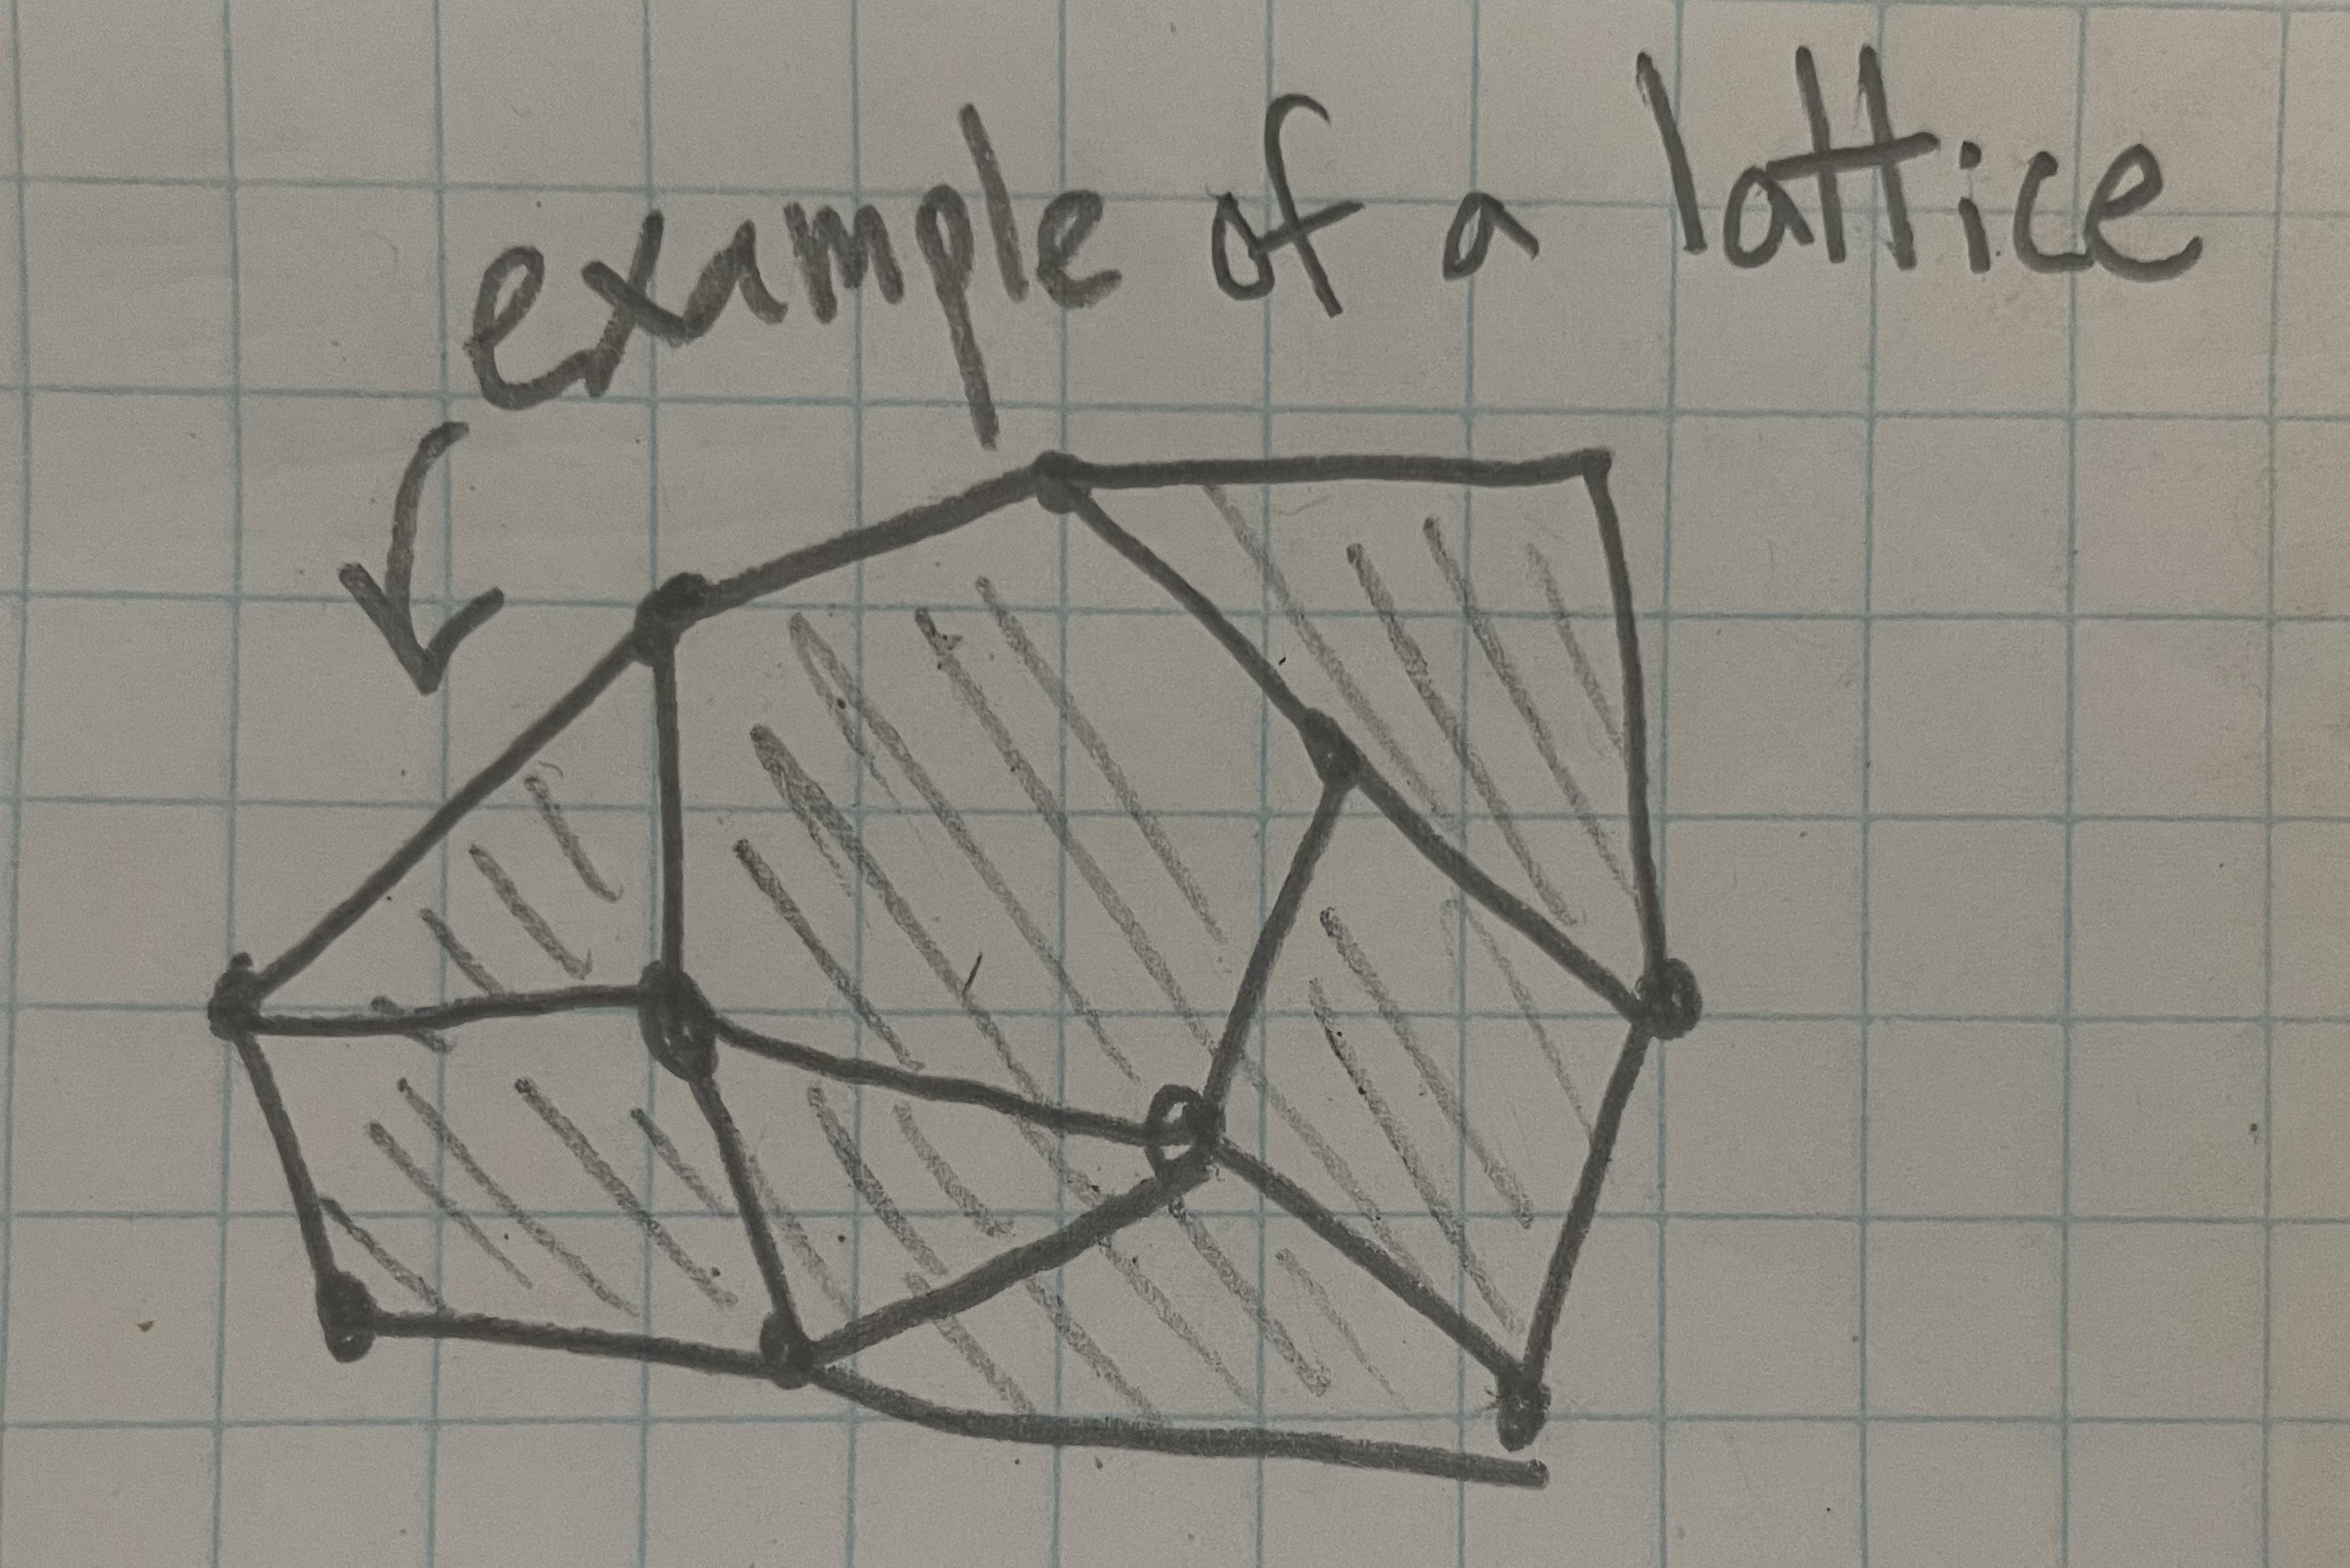
\includegraphics[scale=.04]{lattice-example}
\end{center}
\end{figure}

A lattice is a collection of vertices, edges, and faces connected in some way. To keep in line with the terminology common in topological quantum information, we refer to the faces of our lattices using the French term \textit{plaquette}. Formally, by lattice we mean ``simplicial 2-complex" though there is no need to go into details because we will never be dealing with the subtleties in the definition. Often times we will need to deal with \textit{directed} lattices. These are lattices in which every edge has a direction, which we represent as an arrow on that edge.

Before putting ordered media on a lattice, a good question is \textit{why} we would want to do this. There are two primary reasons. The first is that this will make this Hilbert spaces involved all finite dimensional. This is very important because we have only established quantum mechanics in the finite dimensional case, and working with the continuum limit can be highly complex. The second reason is that in practice, many of the systems physicists deal with are on lattices. For example, the chip of a quantum computer will store its information at finitely many sites, which can correspond to the vertices of some lattice. Many topological systems also arrise from materials which have crystal structures, which are modeled well by a lattice with atoms at the vertices and edges representing the geometry of the crystal.

The best setting for putting our ordered media on a lattice is by first putting on a torus. This helps for several reasons. Firstly, a torus is compact and hence it will add even more finiteness to the problem. Secondly, a torus has nontrivial topology which is useful for seeing the characteristic phenomina of topological order. Thirdly, a torus has no boundary, which helps because boundaries in topological order are subtle and require more work to describe. We denote the torus by $T^2$, and identify it with a square having its opposite sides glued:

\begin{figure}[h]
\begin{center}
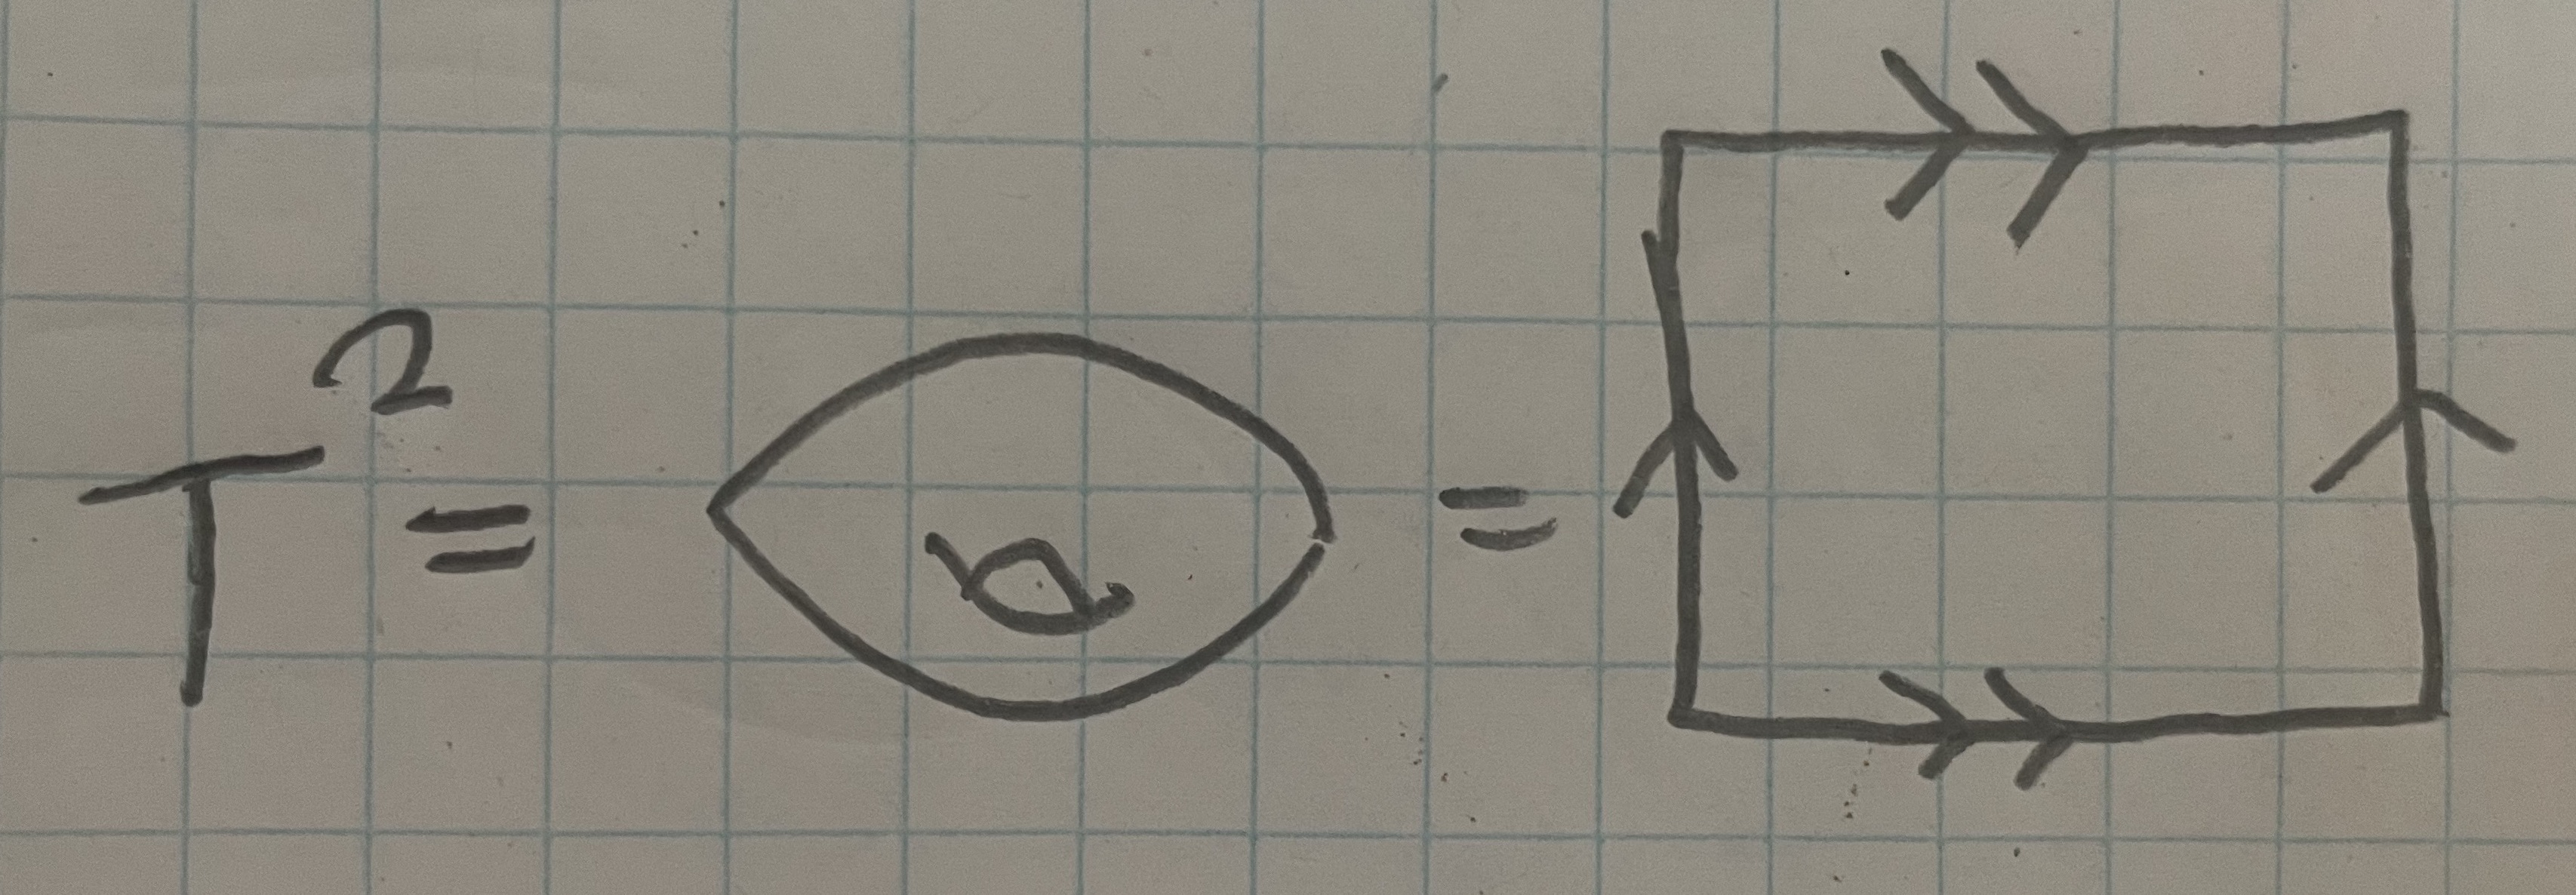
\includegraphics[scale=.04]{torus-definition}
\end{center}
\end{figure}

Ordered media on the torus corresponds to continuous maps $\phi: T^2\to M$ where $M$ is some fixed order space. The steps to transforming a state $\phi$ into a lattice version of itself go as follows:

\begin{enumerate}[Step $\text{1}$(a):]
\item Choose a directed lattice on the torus;
\item Choose a basepoint $m\in M$. Make \textit{local twists} around each vertex so that $\phi(v)=m$ for all vertices $v$ in the lattice.
\item On every edge, write down the winding number of $\phi$ along that edge, as an element of $\pi_1(M,m)$;
\item Forget $\phi$, and remember only the assignment of group elements in $\pi_1(M,m)$ to edges in the lattice.
\end{enumerate}

These steps deserve explanation. Step 1(a) is clear: we choose an arbitrary lattice on the torus. Typically we will choose the square lattice on the torus:

\begin{figure}[h]
\begin{center}
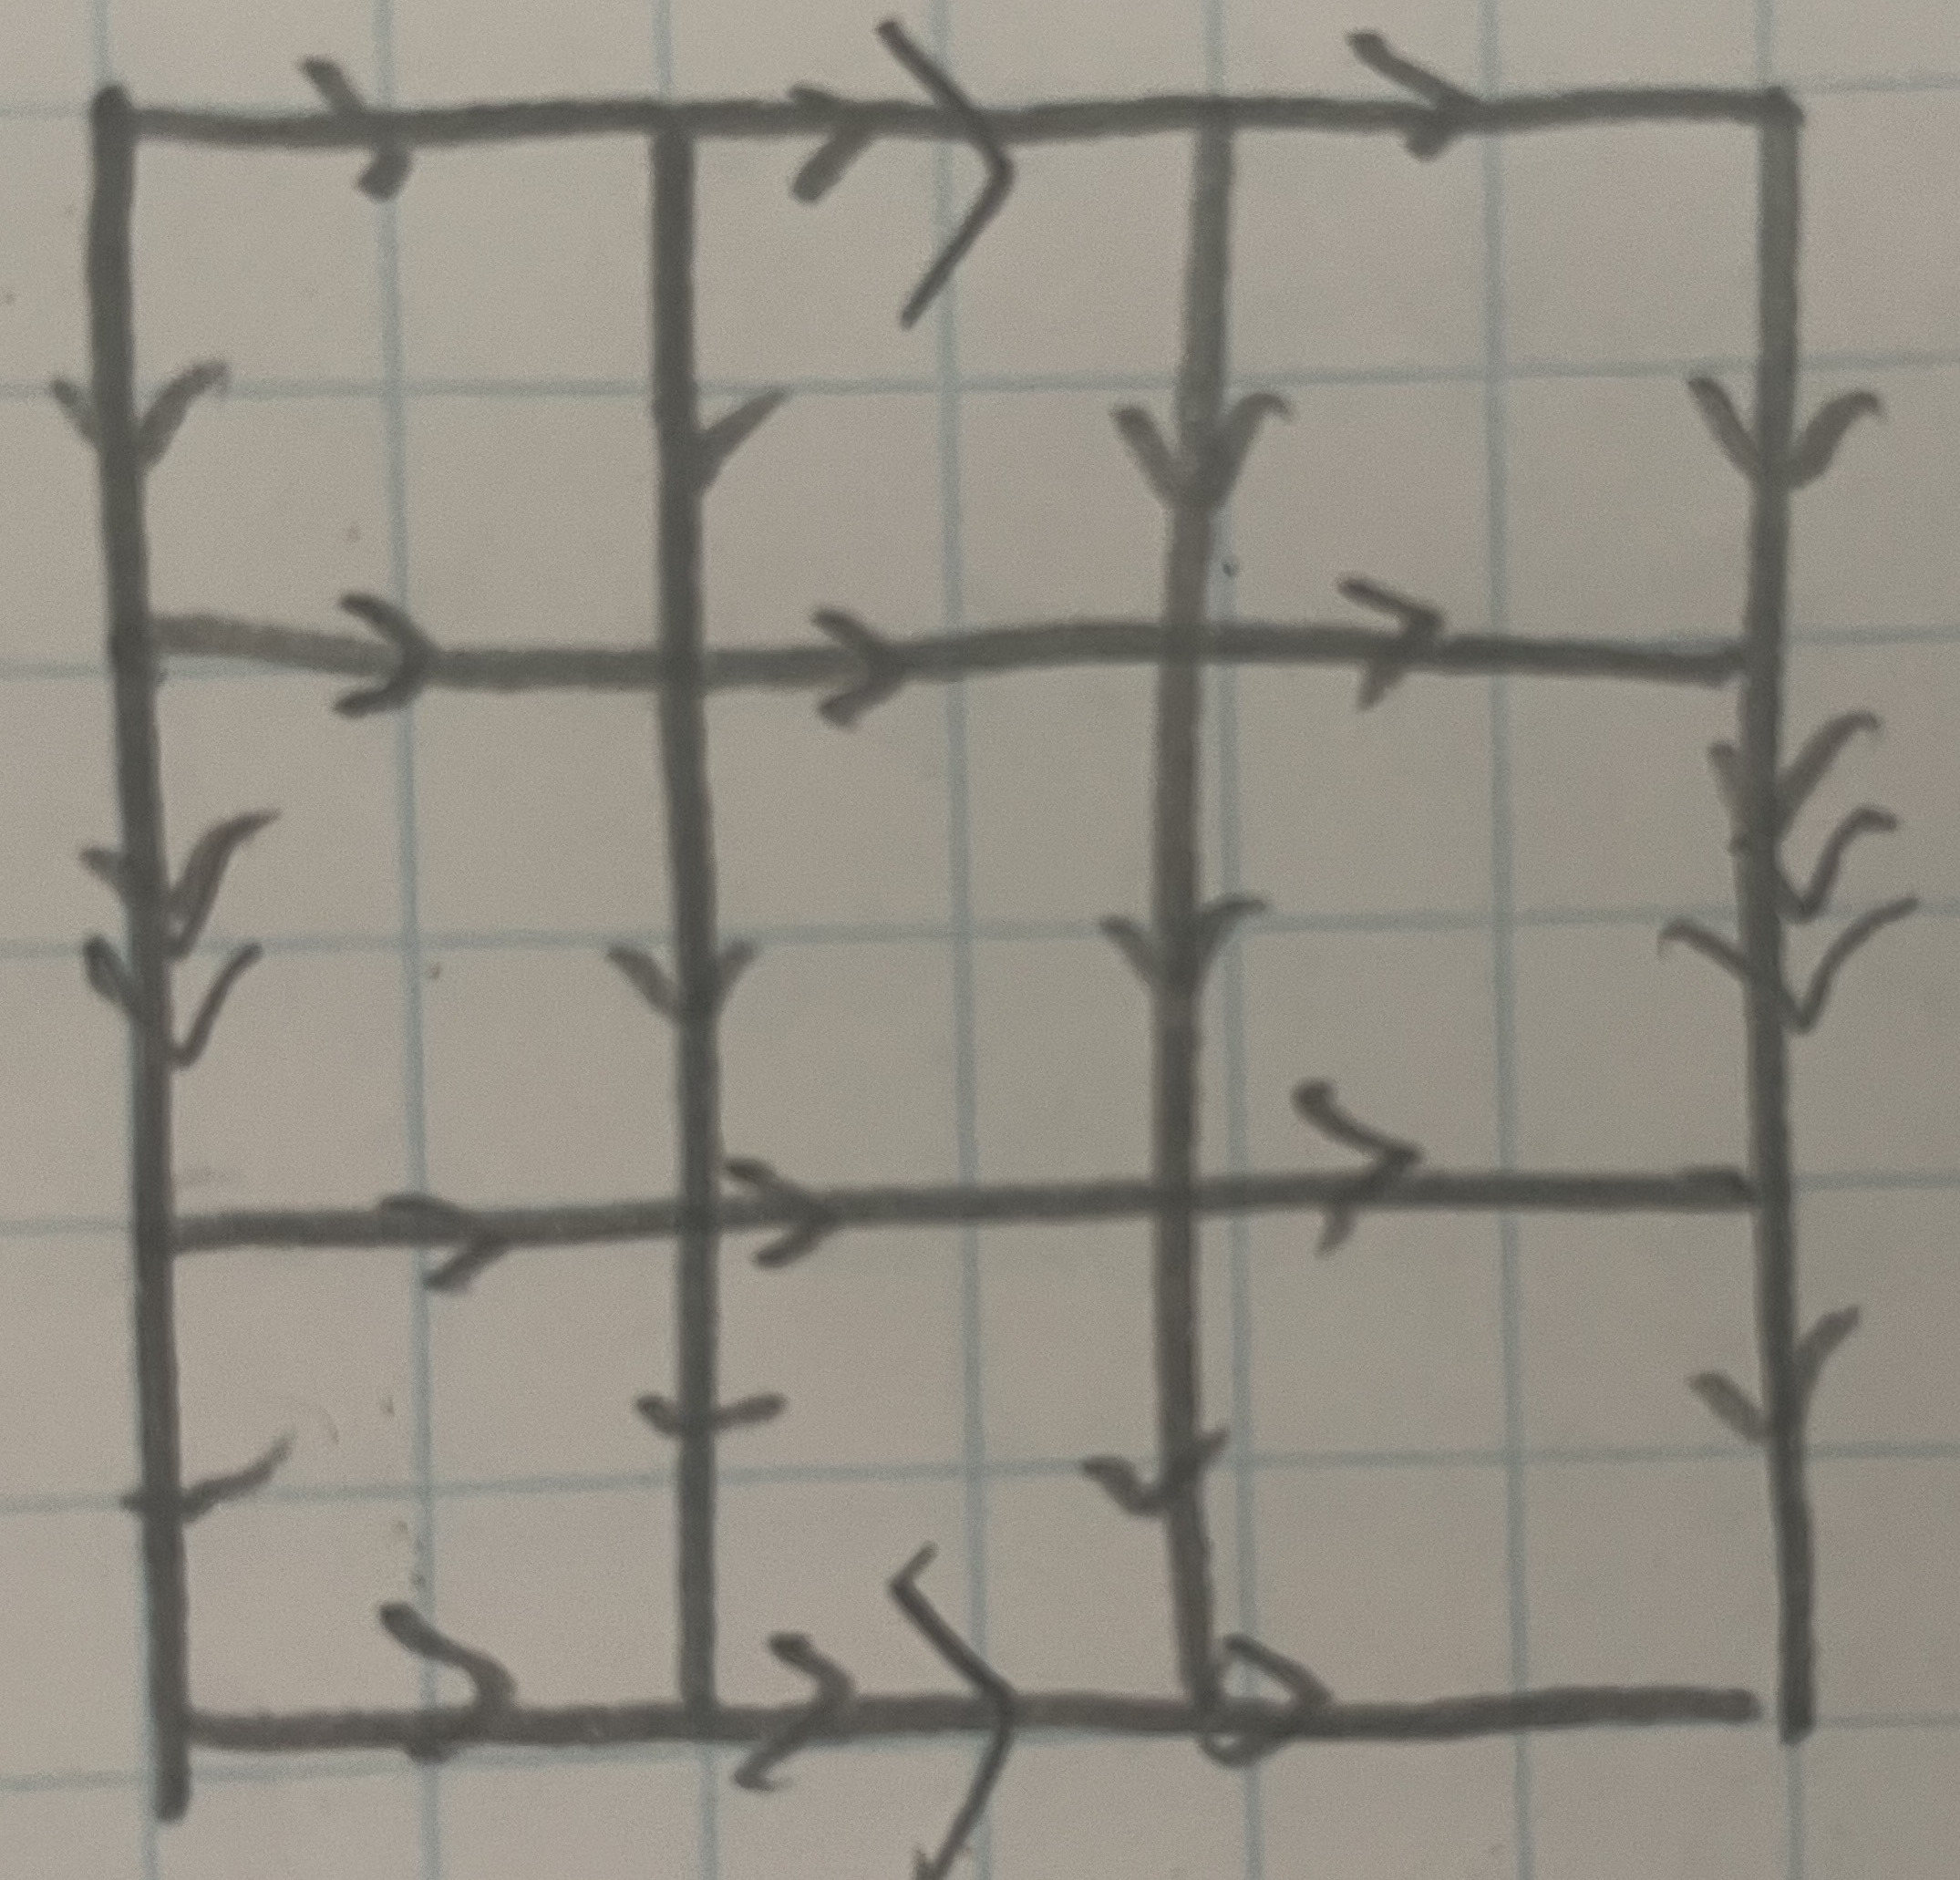
\includegraphics[scale=.04]{torus-lattice}
\end{center}
\end{figure}

Step 1(b) requires more explanation. The picture to imagine is that we take the state $\phi$ and twist its values in small neighborhoods around each vertex to enforce the condition $\phi(v)=m$. Formally, this means choosing another state $\tilde{\phi}$ such that $\tilde{\phi}(v)=m$ for every vertex $v$ of the lattice, and $\tilde{\phi}=\phi$ outside of some chosen small neighborhoods around each vertex. The fact that we can always choose such as state $\tilde{\phi}$ is a consequence of general mathematical principles in homotopy theory. Of course, different choices of $\tilde{\phi}$ will change the final result of our lattice encoding. However because any two choices of $\tilde{\phi}$ can only differ by local changes they can't be \textit{too} different, in a way we will quantify later in the subsection.

Step 1(c) is straightforward. Every edge can be thought of as a path. Pushing forward with $\phi$, this gives us a path in $M$. Since the edge starts and ends at vertices and $\phi$ sends all vertices to $m$, this means that the push forward of our edge gives a loop in $M$ based at $m$. Hence, it gives an element of $\pi_1(M,m)$. We can record this element and attach it as a piece of data associated to the edge.

Step 1(d) is entirely book keeping. It records the fact that we have successfully transformed our continuous data ($\phi:T^2\to M$) into discerete data (an assignement of group elements to edges in a lattice).

A worked example is shown below in the case that $M=S^1$ is the circle:

\begin{figure}[h]
\begin{center}
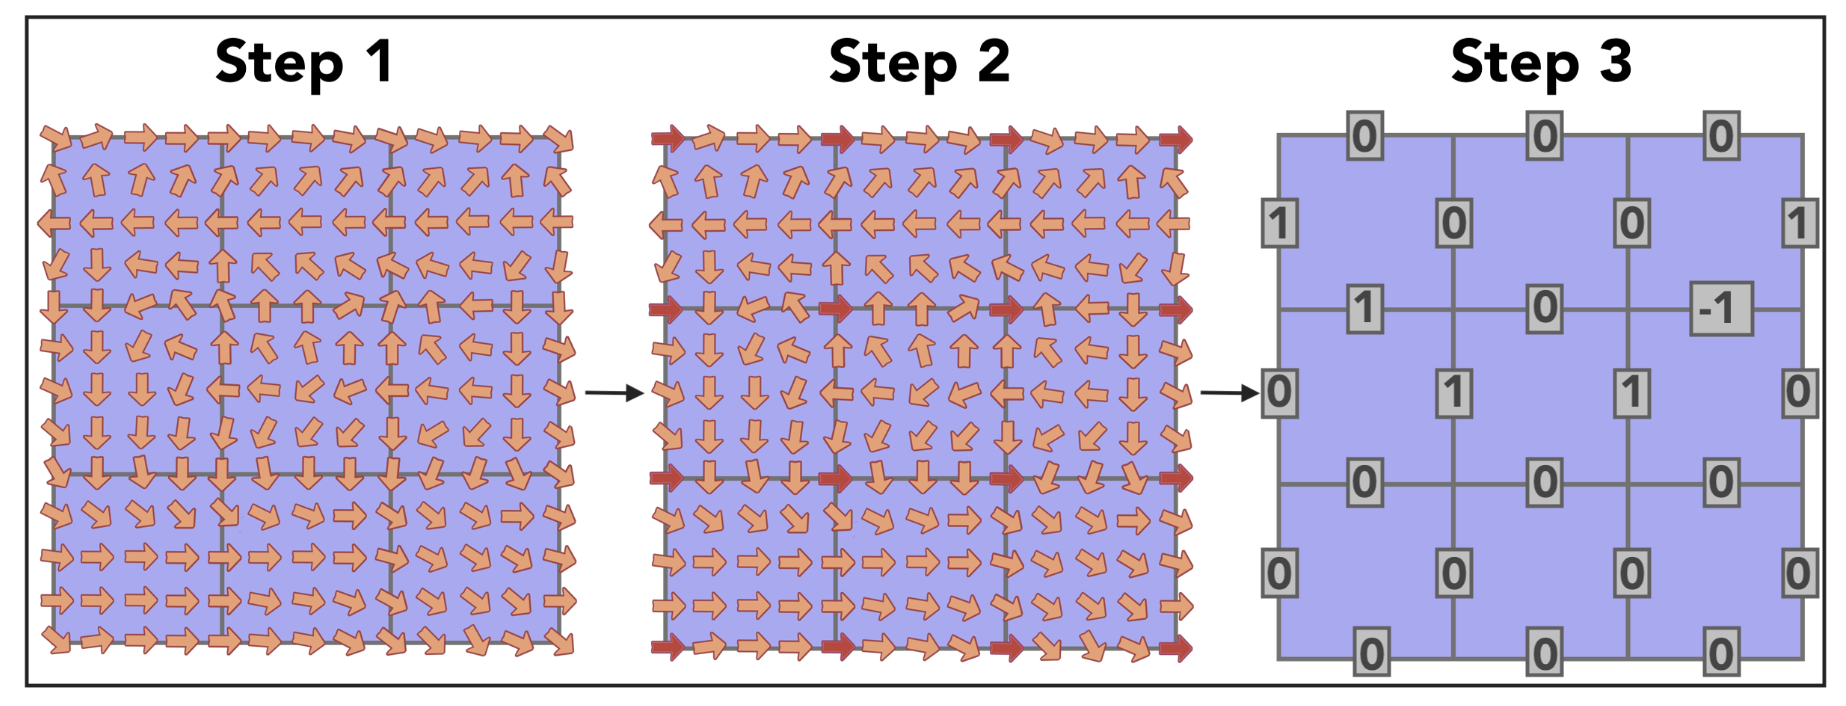
\includegraphics[scale=.3]{full-example}
\end{center}
\end{figure}

We now analyse our encoding of states in ordered media into assignements of group elements in $\pi_1(M,m)$ to edges in the lattice. The first fact from homotopy theory we will use is that these group elements determine the state $\phi$ exactly up to deformations localized within each face. Taking a limit of denser and denser lattices, this means that the group elements will specify $\phi$ up to increasingly local deformations. The intiution is that by taking an infinite lattice limit we should recover $\phi$ up to ``infinitely local deformations", i.e., we recover it exactly. In this way we did a good job with our lattice encoding.

We observe that not every assignement of group elements to edges appears in our construction. There are implicit conditions. In particular, imagine taking the product of the group elements on edges along some contractible loop, taking inverses appropriately so that all the arrows are pointing in the same direction. This product will be equal to the group element associated with the loop around this whole path. The winding number along any contractible path under a continuous map should be trivial. Hence, the product of these group elements should be trivial. In particular, given any plaquette, the ordered product of group elements along its edges should be zero:

\begin{figure}[h]
\begin{center}
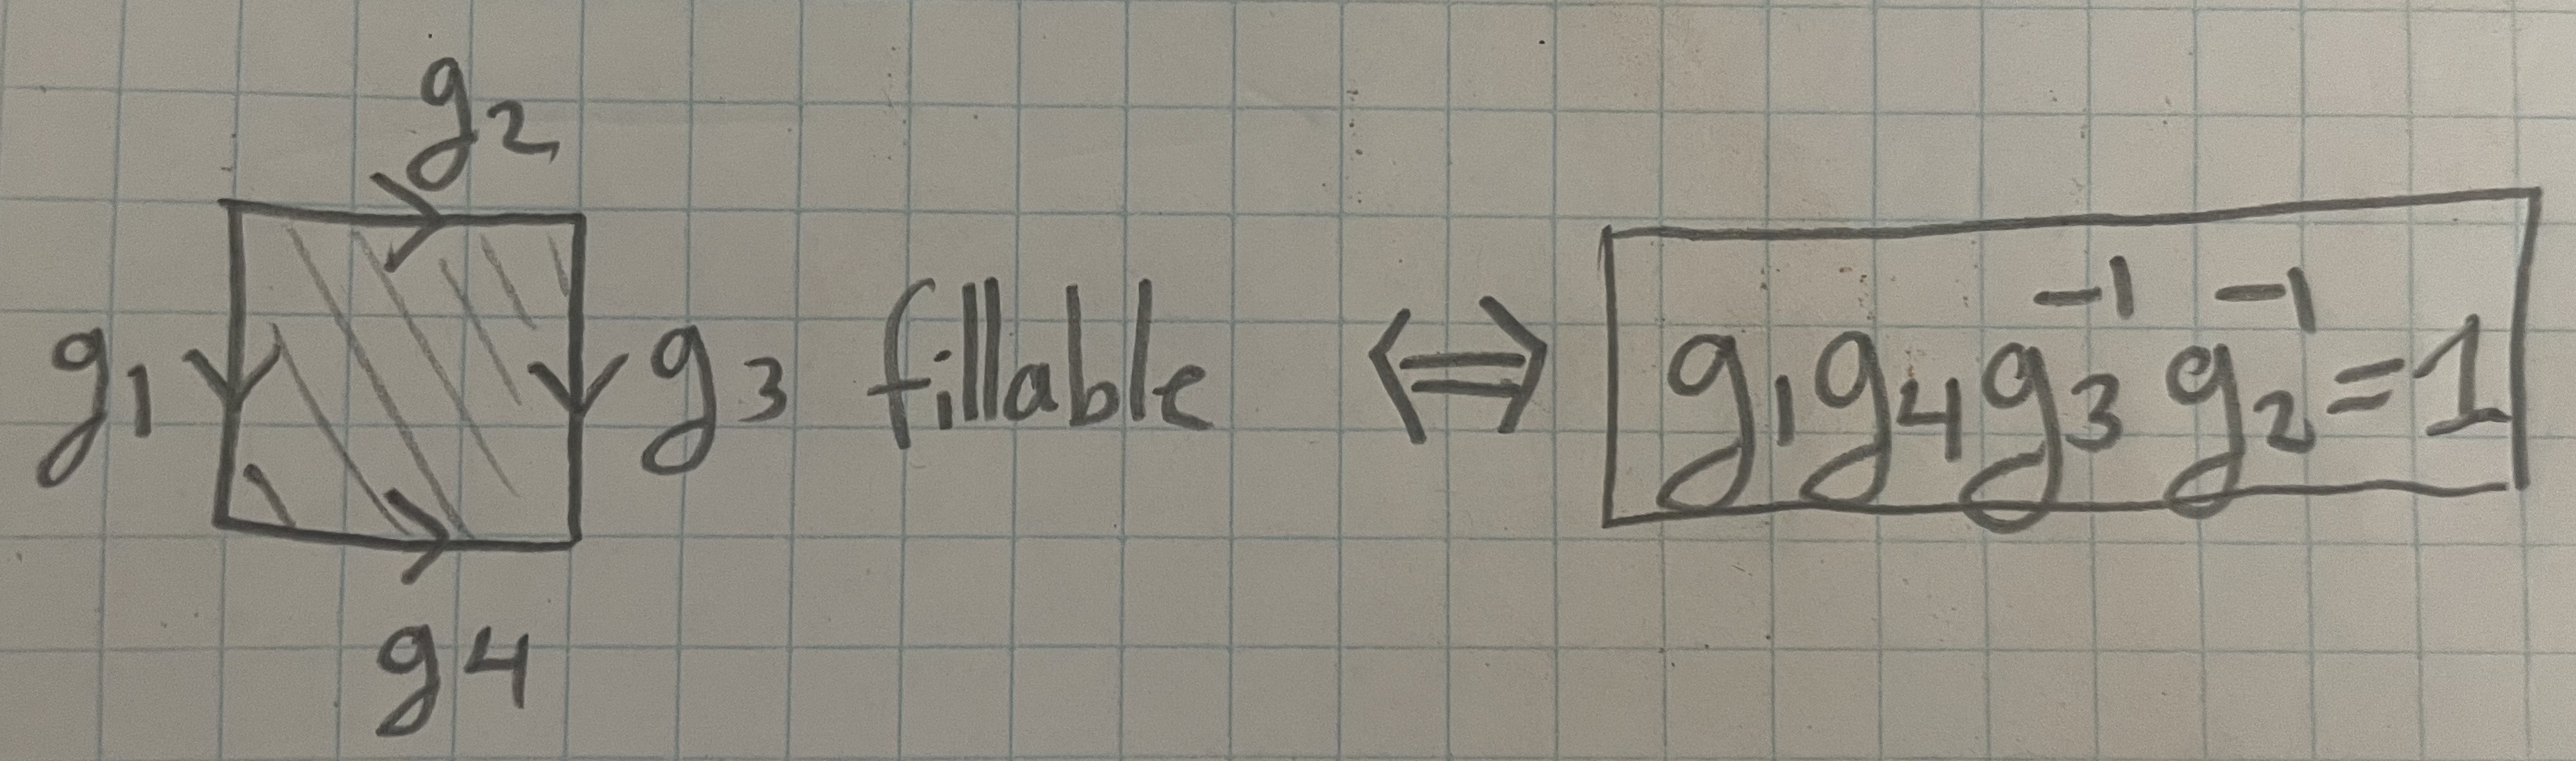
\includegraphics[scale=.06]{plaquette-rule}
\end{center}
\end{figure}

Moreover, \textit{any} coloring of the edges of the lattice by elements of $\pi_1(M,m)$ will come from some map $\phi$ so long as it satisfies the condition above. This is one of the key formulas of the theory. It is in a real sense a lattice version of the continuity condition, since it is \textit{equivalent} to the condition of continuity in the infinite lattice limit. This lattice version of continutity is called \textit{flatness}. Flatness conditions are the most common sort of compatibility conditions which appear when you have local degrees of freedom valued in some group, making this lattice situation very general.

The last thing do deal with in analysing our system is deformation. When analysing states in ordered media, a huge amount of our time was spent on performing continuous deformations. Topological information is defined to be information which is invariant under continuous deformation. What does this correspond to in the lattice model?

Suppose we are given an ordered media state $\phi$ and its corresponding lattice coloring. If we deform $\phi$ in some small neighborhood within a face, this will not change the values along the edges and hence will not change the coloring. If we deform $\phi$ in some small neighborhood around the interior of some edge this also won't change the coloring, because this will correspond to deforming the loop in $M$ induced by going along that edge, and elements of the fundamental group are invariant under deformations of this sort. Another way of seeing that the coloring can't change is that flatness must be preserved - if the group element on the deformed edge changed, it would ruin flatness on the faces it bounds.

Finally, we can consider deforming $\phi$ around some vertex. This certainly \textit{can} impact the coloring. An easy way to compute how it must impact the coloring is by using the fact that the flatness condition must be preserved. Suppose that an incoming edge labled by $g_1$ changes to $g_1 g$ after the deformation. Enforcing flatness along all of the faces touching the vertex allows one to conclude that all incoming edges $g_k$ will get changed to $g_k g$, and all outgoing edges $g_k$ will get changed to $g^{-1}g_k$, as shown below:

\begin{figure}[h]
\begin{center}
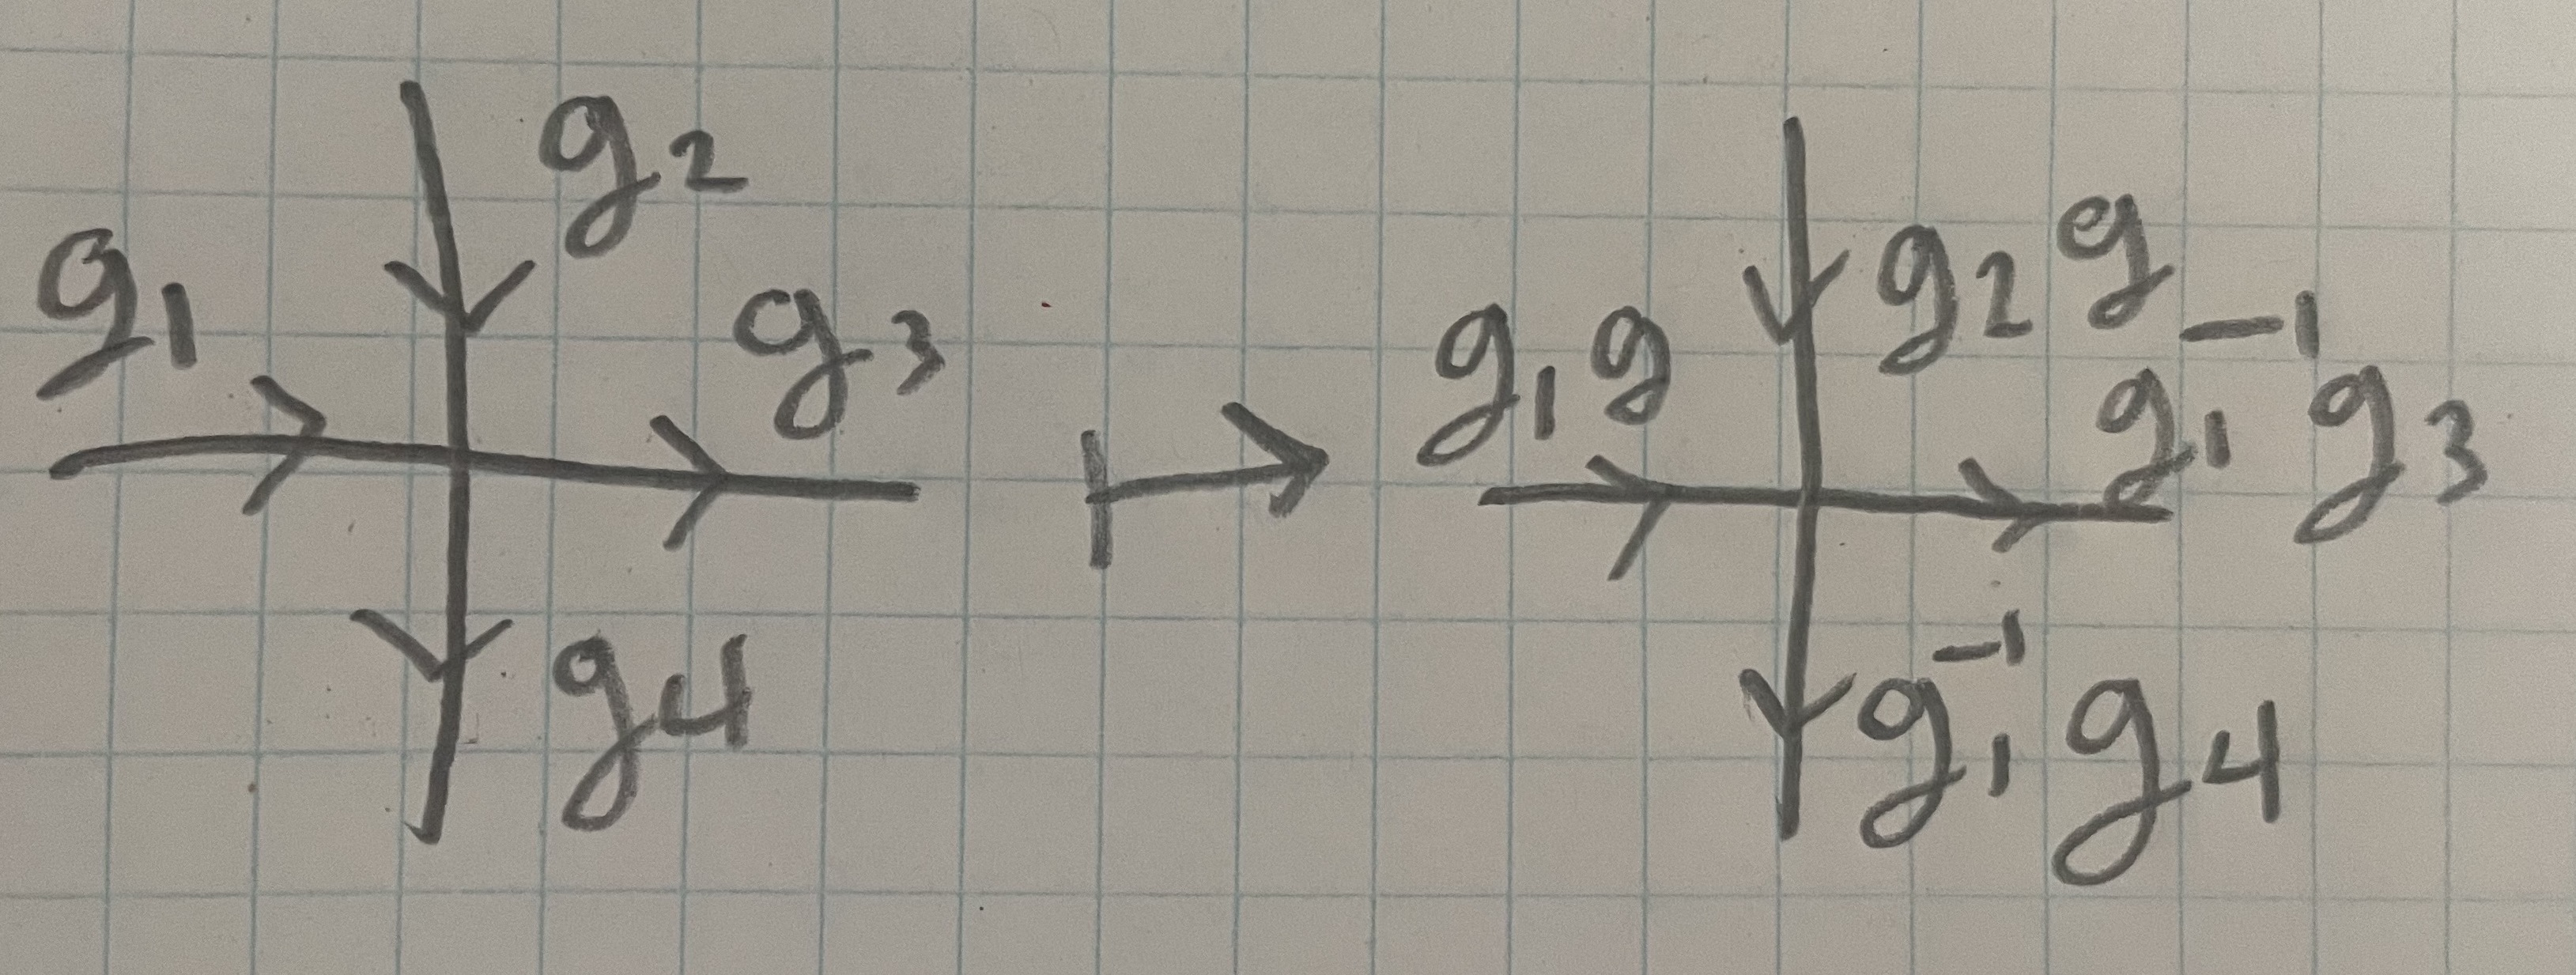
\includegraphics[scale=.04]{gauge-transformation}
\end{center}
\end{figure}

Another way of seeing this result is by anlysing what a deformation of $\phi$ does. The value $\phi(v)$ can move along some loop, starting and ending at $m$. This loop induces some element of the fundamental group, $g\in \pi_1(M,m)$. Performing this deformation exactly acts by precomposing/postcomposing the adject edges with $g$/ $g^{-1}$ accordingly. We can see below a concrete example for $G=S^{1}$:

\begin{figure}[h]
\begin{center}
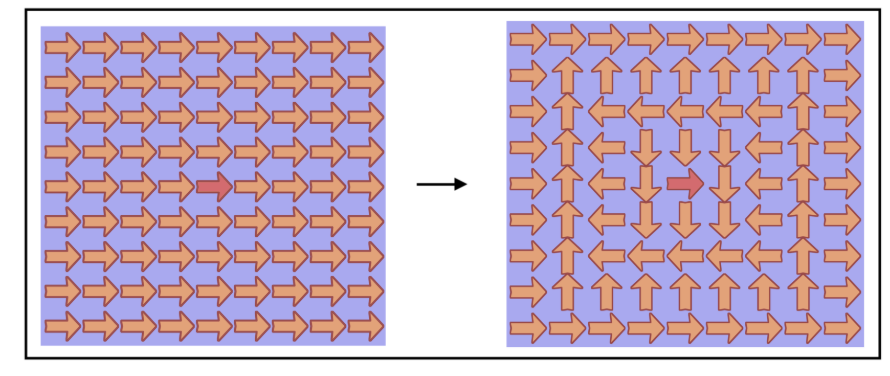
\includegraphics[scale=.45]{twisting}
\end{center}
\end{figure}

Hence, we have a picture for ordered media on the lattice: states correspond to flat colorings of elements of $\pi_1(M,m)$ on a fixed lattice, and continuous deformations correspond to certain vertex actions by elements of $\pi_1(M,m)$.

\subsubsection{From ordered media to gauge theory}

In the previous subsection we showed how to put ordered media on a lattice. In this section we show how to make it quantum, turning it from a classical field theory to a quantum gauge theory. The idea of this jump is as follows. In Section [ref] we obtained an equivalence

$$
\left(\substack{\text{topological information}\\ \text{in ordered media}}\right)=\left(\text{states}\right)/\left(\substack{\text{continuous} \\ \text{deformation}}\right).
$$

It is neccecary to mod out by continuous deformation because there is topoloigcal information in states, but also local degrees of freedom. For instance, the group element assigned to any indivudal edge in ordered media on a lattice can be changed by a gauge transformation and hence is not topologically invariant. The idea of going from ordered media to gauge theory is as follows: gauge theory is what results from ordered media when quantum fluxtuations become so strong that local degrees of freedom are completely washed out and only the topology remains.

The fluxtuations are quantum because we will imagine that our states will evolve in such a way that they are in a superposition of gauge transformations having been applied and not having been applied. Our states in gauge theory will be \textit{equal superpositions over all possible deformations} of a given state. In this way, we are using quantum mechanics as a physical mechanism for quotients. Equivalence classes under deformation will be physically realized as equal superpositions over all possible representatives.

This can all be made completely rigorous. Choose a lattice on the torus, an order space $M$, and a basepoint $m$. We define a Hilbert space

$$\NN=\bigotimes_{\text{edges}}\CC[G].$$

We canonically identify the standard basis of $\NN$ with $G$-colorings of the lattice. Let $C$ be an equivalence class of flat $G$-colorings of $\NN$ up to gauge transformations. There is a corresponding state

$$\ket{C}=\sum_{\gamma \in C}\frac{1}{\sqrt{|C|}}\ket{\gamma}.$$

This state is a normalized equal superposition of representatives of $C$. This defines a sub-Hilbert space

$$\Cc=\text{span}\left\{\left.\ket{C}\right| C\in \text{(flat $G$-colorings)}/\text{(gauge transformations)}\right\}.$$

This Hilbert space $\Cc$ stores the information in our gauge theory.

So far our system is relatively trivial - it is just a Hilbert space, with no Hamiltonian. We connect it back to our original picture of topological order. The space $\Cc$ is the collection of ground states in a topologically ordered system. Above it there is a whole spectrum of other states. This fuller picture with a Hamiltonian adds all of the subtlety and intrigue to the system.

In particular, we observed in Chapter [ref] section [ref] we observed the importants of quasiparticles in ordered media. These formed the heart of our information processing. Similarly, in gauge theory there will be quasiparticles as well, which appear as anyons higher up in the spectrum of the Hamiltonian. Some of these anyons correspond to the classical quasiparticles in ordered media, but other anyons are entirely new features of the system which did not exist before. We will analyse all this in more in the subsection that follows.

\subsubsection{Kitaev quantum double model}

[WORK: not sure if this is readable to someone who skipped the first two sections, but it should be. Something to keep an eye on.]

In this section we will give the Hamiltonian formulation of lattice gauge theory. Seeing as we have moved passed ordered media, we will no longer be working with order spaces and base points. Instead, we will choose an abstract finite group $G$ which replaces $\pi_1(M,m)$. The general picture for creating our Hamiltonian is simple, and follows a very general pattern in quantum theory: instead of enforcing properties rigidly as conditions, we will enforce them enforce properties energetically as terms in a Hamiltonian. The formulation we give below is known as the \textit{Kitaev quantum double model of lattice gauge theory}. It was introduced in Kitaev's seminimal paper on topological quantum information [ref]. It has been studied extensively in the literature by many authors [add more refs].

Choose a directed lattice on the torus. Let

$$\NN=\bigotimes_{\text{edges}}\CC[G]$$

be the HIlbert space of our quantum system. The space $\NN$ has a canonical basis given by $\prod_{\text{edges}}G$, which we  identify with $G$-colorings of the lattice. Given a $G$-coloring $\gamma$, we will denote the corresponding state in $\NN$ by $\ket{\gamma}$. For every plaquette $p$ in the lattice, we define an operator on $\NN$ by

$$B_p\ket{\gamma}=
\begin{cases}
\ket{\gamma} & \gamma \text{ flat at }p\\
0 & \text{otherwise}.
\end{cases}$$

We observe immediately that

$$\sum_{\text{plaquettes }p}(1-B_p)\ket{\gamma}=0 \iff \ket{\gamma} \text{ is flat.}$$

It is in this way that we can enforce properties energetically by adding them as terms to a Hamiltonian. If we chose the Hamiltonian to be $\sum_{\text{plaquettes }p}(1-B_p)$, then the lowest energy eigenspace would exactly correspond to the space spanned by flat $G$-colorings. For every vertex $v$ and group element $g\in G$, we define an operator on $\NN$ by

$$A_{v,g}\ket{\gamma}=\ket{\gamma \text{ acted on by the $g$ gauge action at $v$}}.$$

For any $\ket{\psi}\in \NN$, we call $\ket{\psi}$ \textit{gauge invariant at $v$} if $A_{v,g}\ket{\psi}=\ket{\psi}$ for all $g\in G$. We call $\ket{\psi}$ gauge invariant if it is gauge invariant at $v$ for all vertices $v$. We define

$$A_v=\frac{1}{|G|}\sum_{g\in G}A_{v,g}.$$

We define the Hamiltonian of our system to be

$$H=\sum_{\text{vertices $v$}}(I-A_v)+\sum_{\text{plaquettes $p$}}(I-B_p)$$

where $I$ is the identity operator. We summarize the basic properties of this Hamiltonian below:

\begin{proposition} The following properties of the Kitaev quantum double Hamiltonian hold:

\begin{enumerate}[(a)]
\item The operators $A_v$, $B_p$, and $H$ are Hermitian for all vertices $v$ and plaquettes $p$;
\item The formula $A_{v,g}^{\dagger}=A_{v,-g}$ holds for all vertices $v$ and $g\in G$;
\item All of the operators in the set $\{A_v,B_p\}_{v\in \text{vertices}, p\in \text{plaquettes}}$ commute with every other operator in the set;
\item The eigenstates of $H$ are simultaneous eigenstates of the operators $A_v$, $B_p$;
\item The eigenvalues of the $A_v,B_p$ are all $0$ or $1$;
\item The lowest eigenvalue of $H$ is $0$, and the $0$-eigenspace of $H$ is

$$\Cc=\text{span}\left\{\left.\ket{C}\right| C\in \text{(flat $G$-colorings)}/\text{(gauge transformations)}\right\}.$$

where for we define the ket

$$\ket{C}=\sum_{\gamma \in C}\frac{1}{\sqrt{|C|}}\ket{\gamma}$$

for any equivalence class $C$ of $G$-colorings of the lattice up to gauge transformations.

\end{enumerate}
\end{proposition}
\begin{proof}.[WORK: do proof]
\end{proof}

In particular, the above proposition tells us exactly that we have acheived our goal of realizing a Hamiltonian whose ground states capture the topological information in a lattice-version of ordered media.  The term ``double" in the Kitaev quantum double model refers to the fact that there are two families of terms in $H$ - one family of type $A_v$ and one family of type $B_p$. We can readily compute the dimension of the ground space as follows:

\begin{proposition} Choose a vertex $v$ in the lattice. Every $G$-coloring of the lattice induces an assignment of lattice loops on the torus based at $v$ to elements of $G$, based on taking the oriented winding number along that loop relative to the coloring. This restricts to a map

$$(\text{flat $G$-colorings})\xrightarrow{}\Hom(\pi_1(T^2,v), G)$$

where $\Hom(\cdot,\cdot)$ denotes the space of group homomorphisms between two groups. Any two flat $G$-colorings which differ by gauge transformations will induce the same map in $\Hom(\pi_1(T^2,v), G)$, up to global conjugation by an element of $G$. This induces a bijection

$$(\text{flat $G$-colorings})/(\text{gauge transformations})\xrightarrow{}\Hom(\pi_1(T^2,v), G)/\left(\substack{\text{simultaneous} \\ \text{conjugation}}\right).$$

The set of vectors ${\ket{C}}_{C\in (\text{flat $G$-colorings})/(\text{gauge transformations})}$ is linearly independent. Hence, there is a canonical isomorphism

$$\Cc \xrightarrow{}\CC[\Hom(\pi_1(T^2,v), G)/\left(\substack{\text{simultaneous} \\ \text{conjugation}}\right)]$$

given by taking winding numbers.
\end{proposition}
\begin{proof}.[WORK: give proof]
\end{proof}

The final step in using the above formula is to compute the fundamental group of the torus:

\begin{proposition} $\pi_1(T^2,v)\cong \ZZ^2$ for any vertex $v$. The two loops shown below are generators for $\pi_1(T^2,v)$:

\begin{figure}[h]
\begin{center}
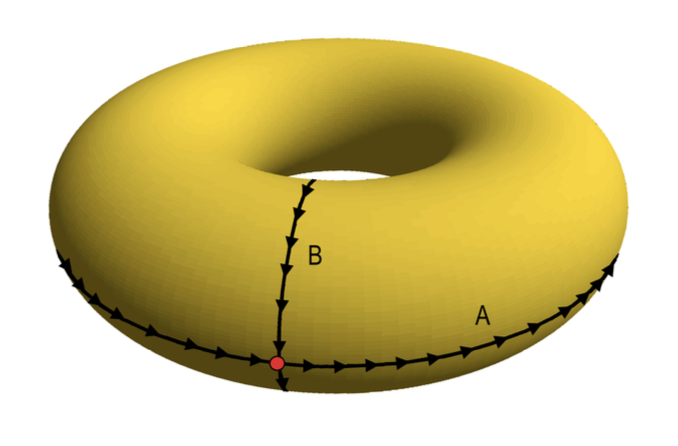
\includegraphics[scale=.3]{torus}
\end{center}
\end{figure}

\end{proposition}
\begin{proof}.[WORK: proof]
\end{proof}

One last observation to make about this ground space is that its ground states really are globally different:

\begin{proposition} Let $L$ be length of the shortest non-contractible loop on the lattice. Let $\gamma_0,\gamma_1$ be non-gauge equivalent flat $G$-colorings of the lattice. There are at least $L$ edges at which $\gamma_0$ and $\gamma_1$ assign different values.
\end{proposition} 
\begin{proof}.[WORK: do proof]
\end{proof}

In particular, if we choose the square lattice on the torus, then the length $L$ of the shortest non-contractible loop is obvioulsy a good measure of linear system size. Proposition [ref] tells us that the number of local changes requires to go from one ground state to another is on the order of $L$. This is exactly the sort of condition we needed in Section [ref] to conclude topological protection in the ground states. Of course, the smallest non-zero eigenvalue of $H$ is at least $1$, which is bounded away from zero and hence there is a system-size independent gap between the ground states and the other states. Hence, we see that $H$ is a good topologically ordered Hamiltonian. 

The excited states of $H$ will be described localized excitations with quasiparticle behavior. Given a state $\ket{\psi}\in \NN$, we will say that a state has an \textit{anyon at vertex $v$} if $A_v\ket{\psi}=0$ and we will say that is \textit{unnoccupied at $p$} if $A_v\ket{\psi}=1$. We say that $\ket{\psi}$ has an \textit{anyon at plaquette $p$} if $B_p\ket{\psi}=0$ and that it is \textit{unnocupied at $p$} if $B_p\ket{\psi}=1$. By Proposition [ref], every energy eigensate is either occupied or unoccupied at every vertex/plaquette. The regions in which $\ket{\psi}$ is unnoccupied are all essentially identical, leading to a homogenous bulk. The sites at which $\ket{\psi}$ is occupied are different, and behave as quasiparticles. We will define operators which move these excitations around.

We think of these anyons as being localized within faces or within arbitrarily small regions around vertices depending on whether they are vertex-type or plaquette-type. We will find that the states of $H$ can be almost entirely described by anyons and their behavior .

[WORK: Add something about local indistinguishability of ground states - reinforce this ``homogenous bulk" idea]

[WORK: Maybe also reinforce that this could be done on \textit{any manifold}, and the gound states would be the same? ]

\subsection{The toric code}

\subsubsection{Exact solution}

In this section we move on to analyzing the Kitaev quantum double model for $G=\ZZ_2$, which is known as the \textit{toric code}. The name toric code comes from the fact that the toric code was first introduced as an error correcting code, and was only later recast as a topologically ordered system [refs]. The toric code is still the basis for many of the most popular error correcting codes [refs]. In a real sense the toric code is the simplest nontrivial topological order. It is a fantastic example which demonstrates almost all of the phenomina of topological order with relatively little work involved. The toric code, and more generally $\ZZ_2$ lattice gauge theories, can be found in all sorts of systems such as [WORK: give examples]. 

We describe the model now. Because $G=\ZZ_2$ is abelian, we will switch to additive notation for our group operation. We choose a \textit{non-oriented} lattice structure on the torus. This lattice does not need to be oriented because changing the direction of edges in the lattice corresponds to taking inverses, and $g=g^{-1}$ for every element $g\in \ZZ_2$. We define

$$\NN = \bigotimes_{\text{edges}}\CC[\ZZ_2]=\bigotimes_{\text{edges}}\CC^2.$$

Here, we identify $\CC[\ZZ_2]$ with $\CC^2$ for convenience, endowing $\CC^2$ with a canonical basis $\{\ket{0},\ket{1}\}$. We call $\CC^2$ a \textit{qubit}, in analogy to ``bits" for classical computing. It is a standard two-level quantum system. Most quantum computers are based on qubits, which makes the toric code especially accessable to practical implementation as an error correcting code. The definition of the Hilbert space $\NN$ can be summarized as putting a qubit on every edge of the lattice. The Hamiltonian is

$$H=\sum_{\text{vertices }v}(1-A_v)+\sum_{\text{plaquettes }p}(1-B_p).$$

We unpack the general definitions of $A_v$ and $B_p$ for the toric code. The operator $A_{v,0}$ is the identity. The operator $A_{v,1}$ acts by a gauge transformation,

\begin{figure}[h]
\begin{center}
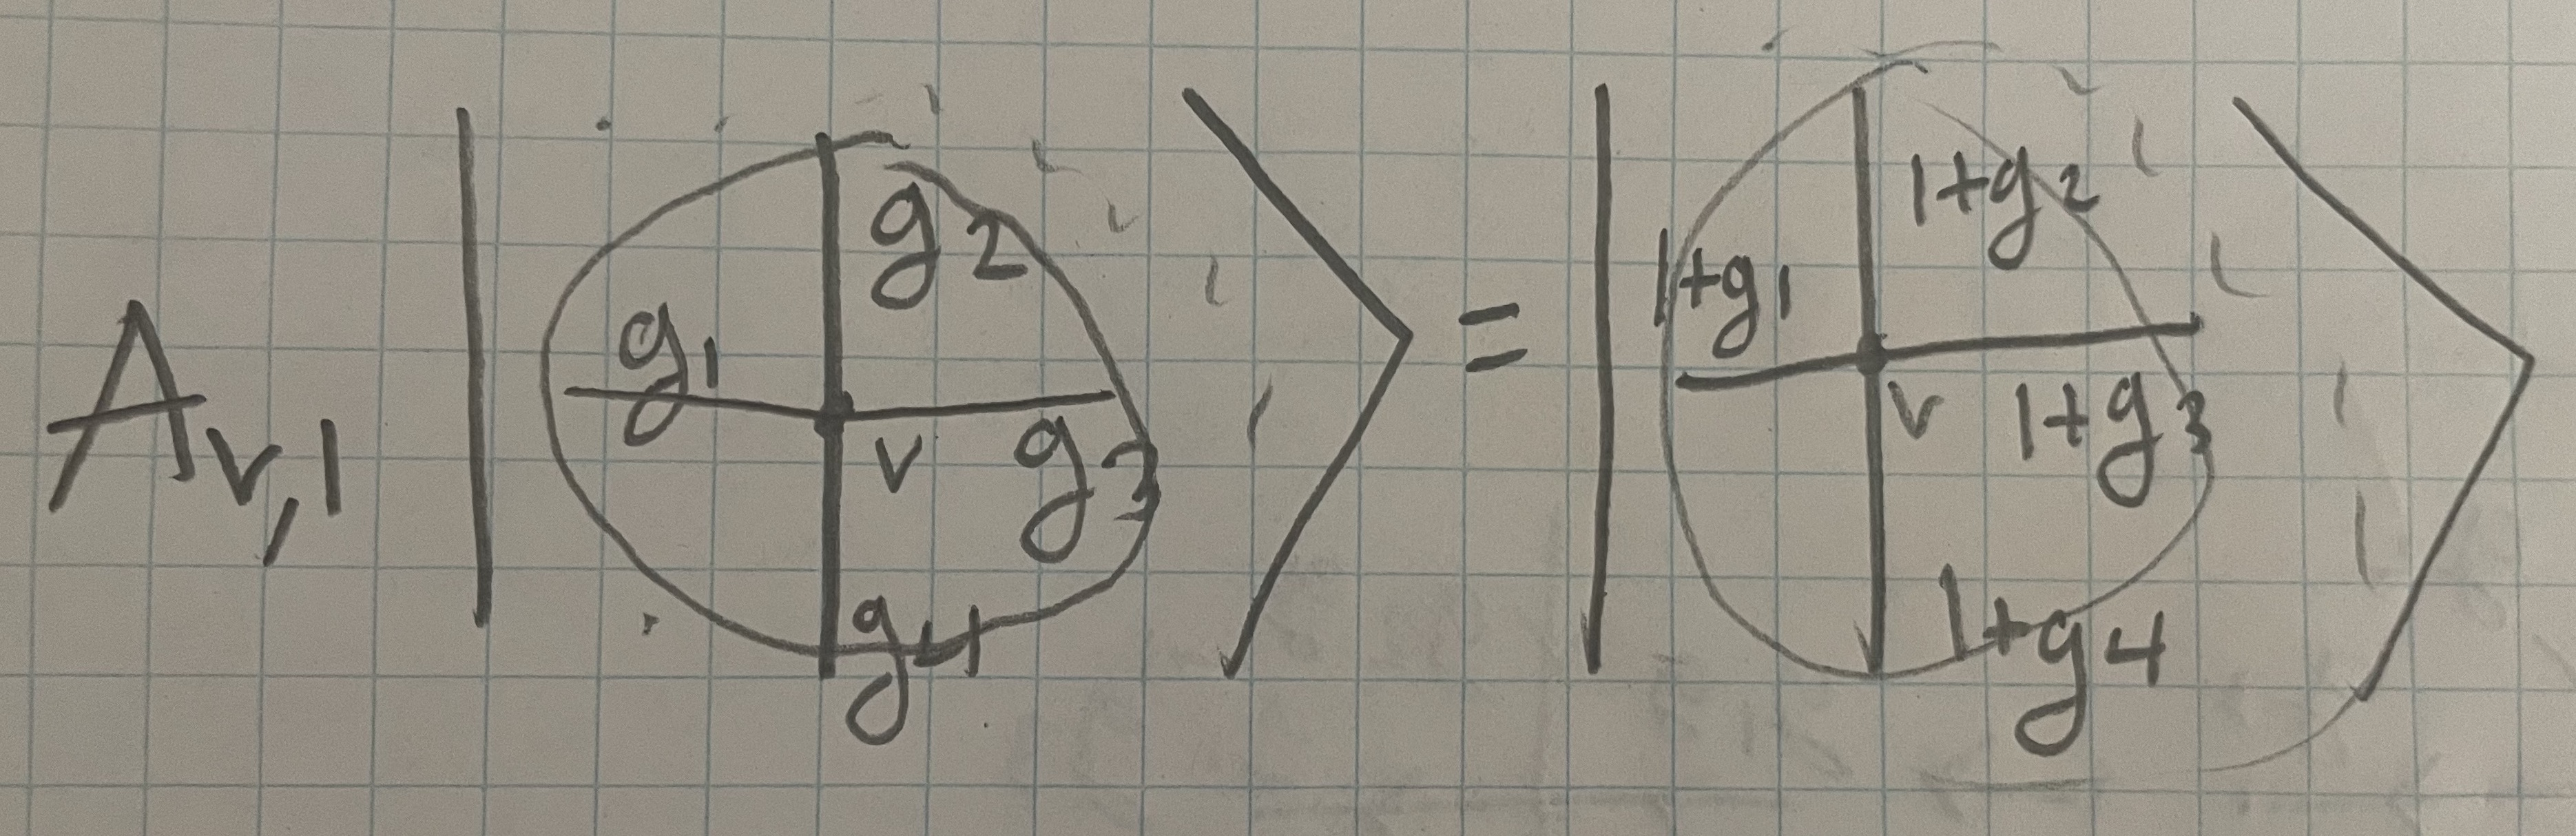
\includegraphics[scale=.04]{Av-gauge-action}
\end{center}
\end{figure}

Defining

\begin{align*}
\sigma_X:\CC^2&\xrightarrow{}\CC^2\\
\ket{0}&\mapsto \ket{1}\\
\ket{1}&\mapsto \ket{0}
\end{align*}

we thus find that

\begin{align*}
A_{v,1}=\bigotimes_{\substack{\text{edges} \\ \text{touching }v}}\sigma_X, && A_v=\frac{1}{2}\left(I + A_{v,1}\right).
\end{align*}

Moving on to $B_p$, we recall that

\begin{figure}[h]
\begin{center}
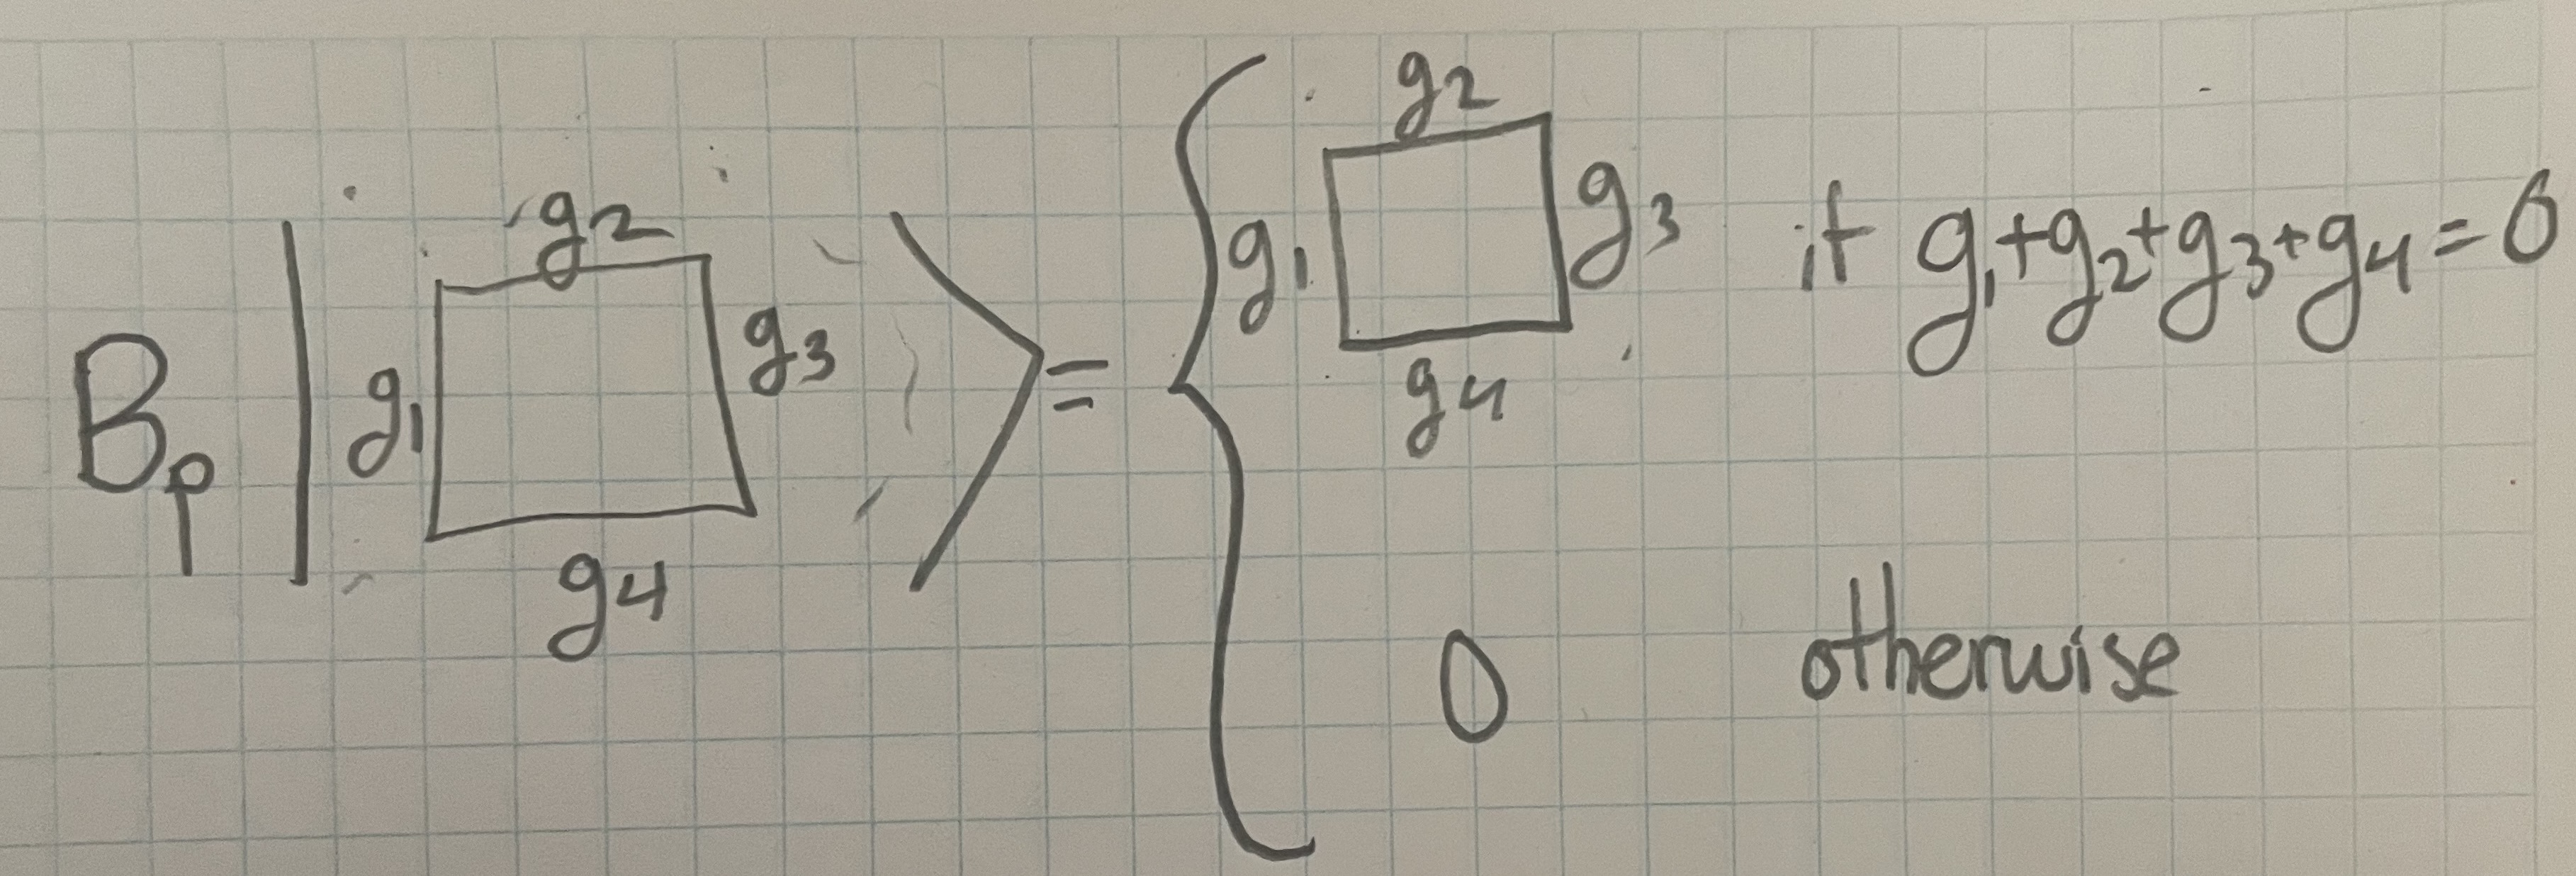
\includegraphics[scale=.04]{Bp-definition}
\end{center}
\end{figure}

In the present case, $B_p$ has a more workable expressing that is symmetric to our description of $B_p$. Define

\begin{align*}
\sigma_Z:\CC^2&\xrightarrow{}\CC^2.\\
\ket{0}&\mapsto \ket{0}\\
\ket{1}&\mapsto -\ket{1}
\end{align*}

Philosophically, it is useful to interpret $\sigma_Z$ as acting as $\ket{g}\mapsto \chi(g)\ket{g}$ where $\chi:\ZZ_2\to\CC^\times$ is the unique nontrivial character of $\ZZ_2$, $\chi(0)=1$, $\chi(1)=-1$. Since $\chi$ is a group isomorphism, for any $g_1,g_2,g_3,g_3\in G$ we have an equivalence

$$g_1+g_2+g_3+g_3=0 \iff \chi(g_1)\chi(g_2)\chi(g_3)\chi(g_4)=1.$$

Defining an auxillary $B_{p,1}$, we thus find the following expression for $B_p$:

\begin{align*}
B_{p,1}=\bigotimes_{\substack{\text{edges} \\ \text{bounding }p}}\sigma_Z, && B_p=\frac{1}{2}\left(I + B_{p,1}\right).
\end{align*}

For simplicity, we will often rewrite the Hamiltonian as

$$H=\frac{1}{2}\sum_{\text{vertices }v}(1-A_{v,1})+\frac{1}{2}\sum_{\text{plquettes }p}(1-B_{p,1}).$$

The matrices $\sigma_X$ and $\sigma_Z$ we defined are known as \textit{Pauli matrices}. They are extremely common across formulae in quantum mechanics - this is another reason that the toric code is so ammenable to error correction applications. The basic properties of these matrices are summarized below:

\begin{proposition}$\,$
\begin{enumerate}[(a)]
\item The operators $\sigma_X$ and $\sigma_Z$ are simultaneously unitary and Hermitian;
\item $\sigma_X^2=\sigma_Z^2=I$;
\item $\sigma_X \sigma_Z = - \sigma_Z \sigma_X$;
\end{enumerate}
\end{proposition}
\begin{proof}.[WORK: do proof]
\end{proof}

An important thing to note is that $A_{v,1}$ and $B_{p,1}$ commute, despite the fact that $\sigma_X$ and $\sigma_Z$ anticommute. The fact that they commute follows from Proposition [ref], though it fruitful to reavulate that proposition in this present context. The important fact is that given any vertex $v$ on the exterior of any face touching $p$,  there are an \textit{even number} of edges which both touch $v$ and bound $p$. Hence, the number of tensor factors in which $A_{v,1}$ and $B_{p,1}$ anticommute is even, and hence overall they commute.

The last step in reinterpreting our general theory of Kitaev quantum double models to the toric code is computing the ground space. We observe that since $\ZZ_2$ is abelian acting by conjugation does nothing, and hence

$$\Hom(\pi_1(T^2,v), \ZZ_2)/\left(\substack{\text{simultaneous} \\ \text{conjugation}}\right)=\Hom(\pi_1(T^2,v), \ZZ_2).$$

Seeing as we are no longer modding out by conjucation, the group operation on $\ZZ_2$ extends to a group operation on $\Hom(\pi_1(T^2,v), \ZZ_2)$. Hence this space forms an abelian group, which we denote

$$H^1(T^2,\ZZ_2)=\Hom(\pi_1(T^2,v), \ZZ_2)=(\text{flat $\ZZ_2$-colorings})/(\text{gauge transformations}).$$

[WORK: maybe set notation and write out four elements explicitely? Might be too much.]

This is the \textit{cohomology group of $T^2$ with coeffecients in $\ZZ_2$}. Since $\pi_1(T^2,v)\cong \ZZ^2$, we conclude that

$$H^1(T^2,\ZZ_2)\cong \ZZ_2^2.$$

Hence, we obtain the following:

\begin{proposition} The $0$-eigenspace of $H$ is four dimensional. It is spanned by the vectors

$$\ket{C}=\frac{1}{\sqrt{|C|}}\sum_{\gamma\in C}\ket{\gamma}$$

for $C\in H^1(T^2,\ZZ_2)$.
\end{proposition}
\begin{proof}.[WORK: do proof]
\end{proof}

\subsubsection{Anyons in the toric code}

We now turn to analysing anyons in the toric code - localized excitations which behave as quasiparticles. Keeping in line with general principles about the Kitaev quantum double model, given a state $\ket{\psi}\in \NN$ we say that there is an anyon at vertex $v$ if $A_v\ket{\phi}=0$, and we say that vertex $v$ is unnoccupied if $A_v\ket{\phi}=\ket{\psi}$. Similarly, we say that there is a quasiparticle at plaquette $p$ if $B_p\ket{\psi}=0$ and that plaquette $p$ is unoccupied if $B_p\ket{\psi}=\ket{\psi}$. In summary,

\begin{align*}
\text{$\ket{\psi}$ has anyon at $v$}\iff A_v\ket{\psi}&=0 \iff A_{v,1}\ket{\psi}=-\ket{\psi}\\
\text{$\ket{\psi}$ has anyon at $p$}\iff B_p\ket{\psi}&=0 \iff B_{p,1}\ket{\psi}=-\ket{\psi}.
\end{align*}

We call the anyons at vertices \textit{vertex type} or \textit{$Z$-type} anyons, and we call the anyons at faces \textit{plaquette type} or \textit{$X$-type} anyons. Our key observation is that applying $\sigma_X$ and $\sigma_Z$ gives total control over the behavior of anyons. Namely, applying $\sigma_X$ or $\sigma_Z$ in the correct circumstates corresponds to creating, moving, and fusing anyons. This comes from the following computation. Given an edge $e$ in the lattice and an operator $U:\CC^2\to \CC^2$, denote by $(U)_e:\NN\to\NN$ the operator which applies $U$ on the tnesor factor of $\CC^2$ at edge $e$. We compute the following:

\begin{lemma} For any vertex $v$, edge $e$, plaquette $p$, we have

\begin{align*}
A_v  (\sigma_X)_e=(\sigma_X)e A_v, && B_p (\sigma_Z)_e=(\sigma_Z)e B_p,
\end{align*}

\begin{equation*}
A_v (\sigma_Z)_e=
\begin{cases}
- (\sigma_Z)_e A_v & \text{if $e$ touches $v$}\\
(\sigma_Z)_e A_V & \text{otherwise}
\end{cases}
\end{equation*}

and

\begin{equation*}
B_p (\sigma_X)_e=
\begin{cases}
- (\sigma_X)_e B_p & \text{if $e$ bounds $p$}\\
(\sigma_X)_e B_p & \text{otherwise}
\end{cases}
\end{equation*}


\end{lemma}
\begin{proof}.[WORK: do proof]
\end{proof}

Suppose that $\ket{\psi}$ is a state with no anyons -that is, a ground state. Given any edge $e$, the state $(\sigma_X)_e \ket{\psi}$ will not be a ground state. In particular, it will no longer commute with $B_p$ at the two plaquettes touching $e$. In this way, applying $\sigma_X$ to the edge $e$ spontanously created a pair of $X$-type anyons around it. Similarly, the staet $(\sigma_Z)_e\ket{\psi}$ will no longer commute with the $A_v$ operators at the two vertices touching $e$. Hence applying $\sigma_Z$ to the edge $e$ spontaneously created a pair of $Z$-type anyons around it. Applying further $\sigma_Z$ and $\sigma_X$ operators has the effect of chaning the quasiparticle content of the state further. If both the adjacent sites are unnoccupied then applying the operator will create a pair of anyons, if one of the sites is occupied then applying the operator will move the anyon from the occupied site to the unoccupied site, and if both of the sites are occupied then applying the operator will annhilate the anyons. We demonstrate this in some examples below

\begin{figure}[h]
\begin{center}
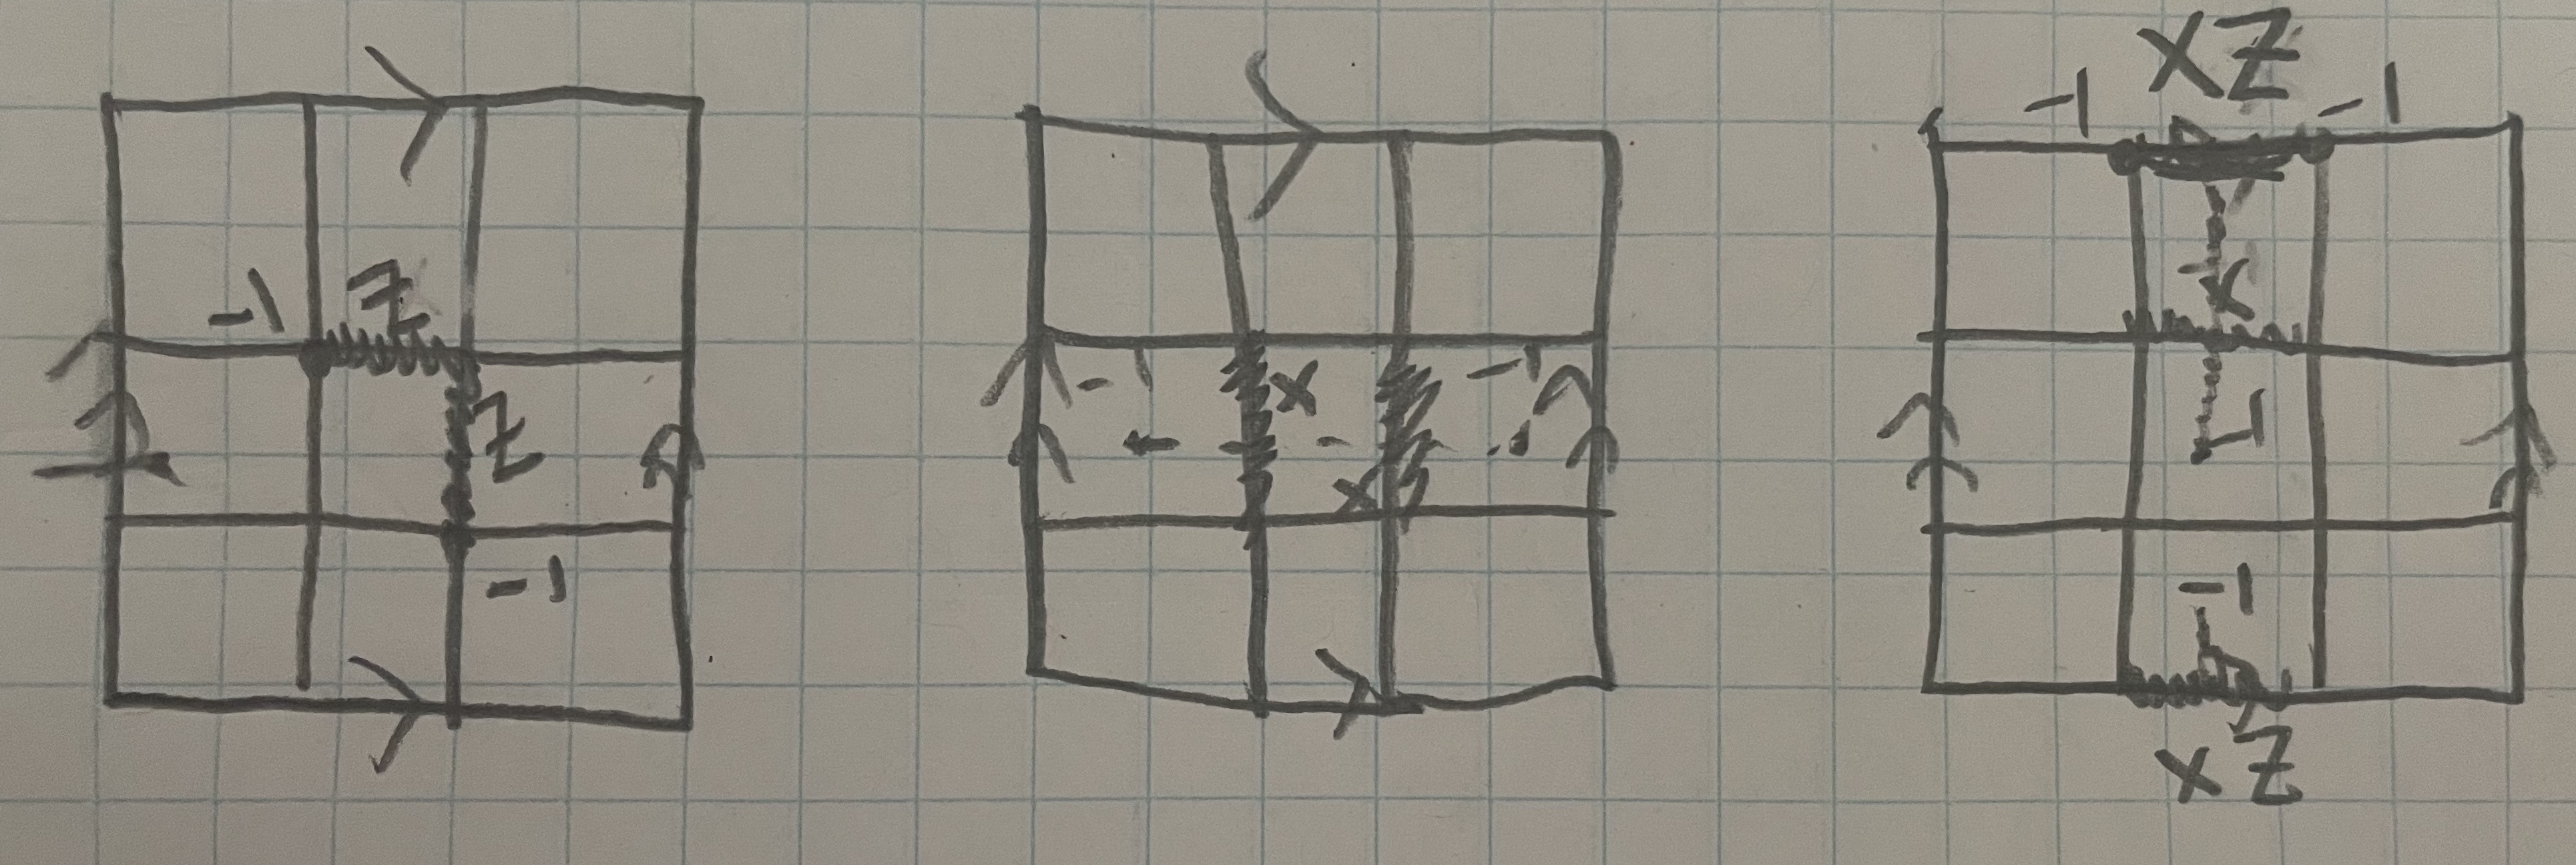
\includegraphics[scale=.04]{anyon-examples}
\end{center}
\end{figure}

We can use this idea of anyons to fully solve the toric code. We introduce some terminology and notation. Given an energy eigenstate $\ket{\psi}$, there is an associated map $\lambda: (\text{vertices})\sqcup (\text{plaquettes})\to \{\pm 1\}$ defined by the relation $A_{v,1}\ket{\psi}=\lambda(v)\ket{\psi}$, $B_{p,1}\ket{\psi}=\lambda(p)\ket{\psi}$. We call maps $\lambda: (\text{vertices})\sqcup (\text{plaquettes})\to \{\pm 1\}$ \textit{syndromes}, and the map associated to $\ket{\psi}$ is the \textit{syndrome of $\ket{\psi}$}. These syndromes allow us to speak intelligently about the locations of anyons within a state. For any syndrome $\lambda$, define

$$\NN_\lambda=\left\{\ket{\psi}\left| \text{syndrome of $\ket{\psi}$ is $\lambda$}\right.\right\}.$$

It is clear that

$$\NN=\bigoplus_{\text{syndromes $\lambda$}}\NN_\lambda$$

and

$$\C=\NN_{\sigma(v)=\sigma(p)=1 \,\, \forall v,p}$$

The following proposition and its proof give a complete description of the eigenstates and eigenvalues

\begin{proposition}The dimension of $\NN_{\lambda}$ is $4$ if the number of vertices $v$ and plaquettes $p$ for which $\lambda(v)=-1$ and $\lambda(p)=-1$ are both even, and the dimension of $\NN_{\lambda}$ is zero otherwise. The eigenvalue of every vector in $\NN_{\lambda}$ is equal to the total number of anyons in the system.
\end{proposition}
\begin{proof}.[WORK: do proof]
\end{proof}

The anyons in the toric code are interesting objects in their own right. For example, we can analyse what happens when we braid anyons. Suppose that $\ket{\psi}$ is a state with one $X$-type anyon and one $Z$-type anyon at adjacent sites. That is, the $X$-type anyon is at a vertex $v$ touching a plaquette $p$. Moving the $Z$-type anyon around the $X$-type anyon corresponds to applying $\sigma_Z$ to the edges around the $X$-type anyone one by one. In other words, the operator required to move the $Z$-type anyon is the tensor product of $\sigma_Z$ along the edges bounding $p$. However, by definition, this operator is exactly $B_{p,1}$. We know that $B_{p,1}\ket{\psi}=-\ket{\psi}$ by the definition of having an anyon at plaquette $p$. Hence, we conclude that \textit{moving a $Z$-type anyon around an $X$-type anyon results in a phase of $-1$}. Similarly, we oberve that moving a $Z$-type anyon around an $X$-type anyon also results in a phase of $-1$, as shown below:

\begin{figure}[h]
\begin{center}
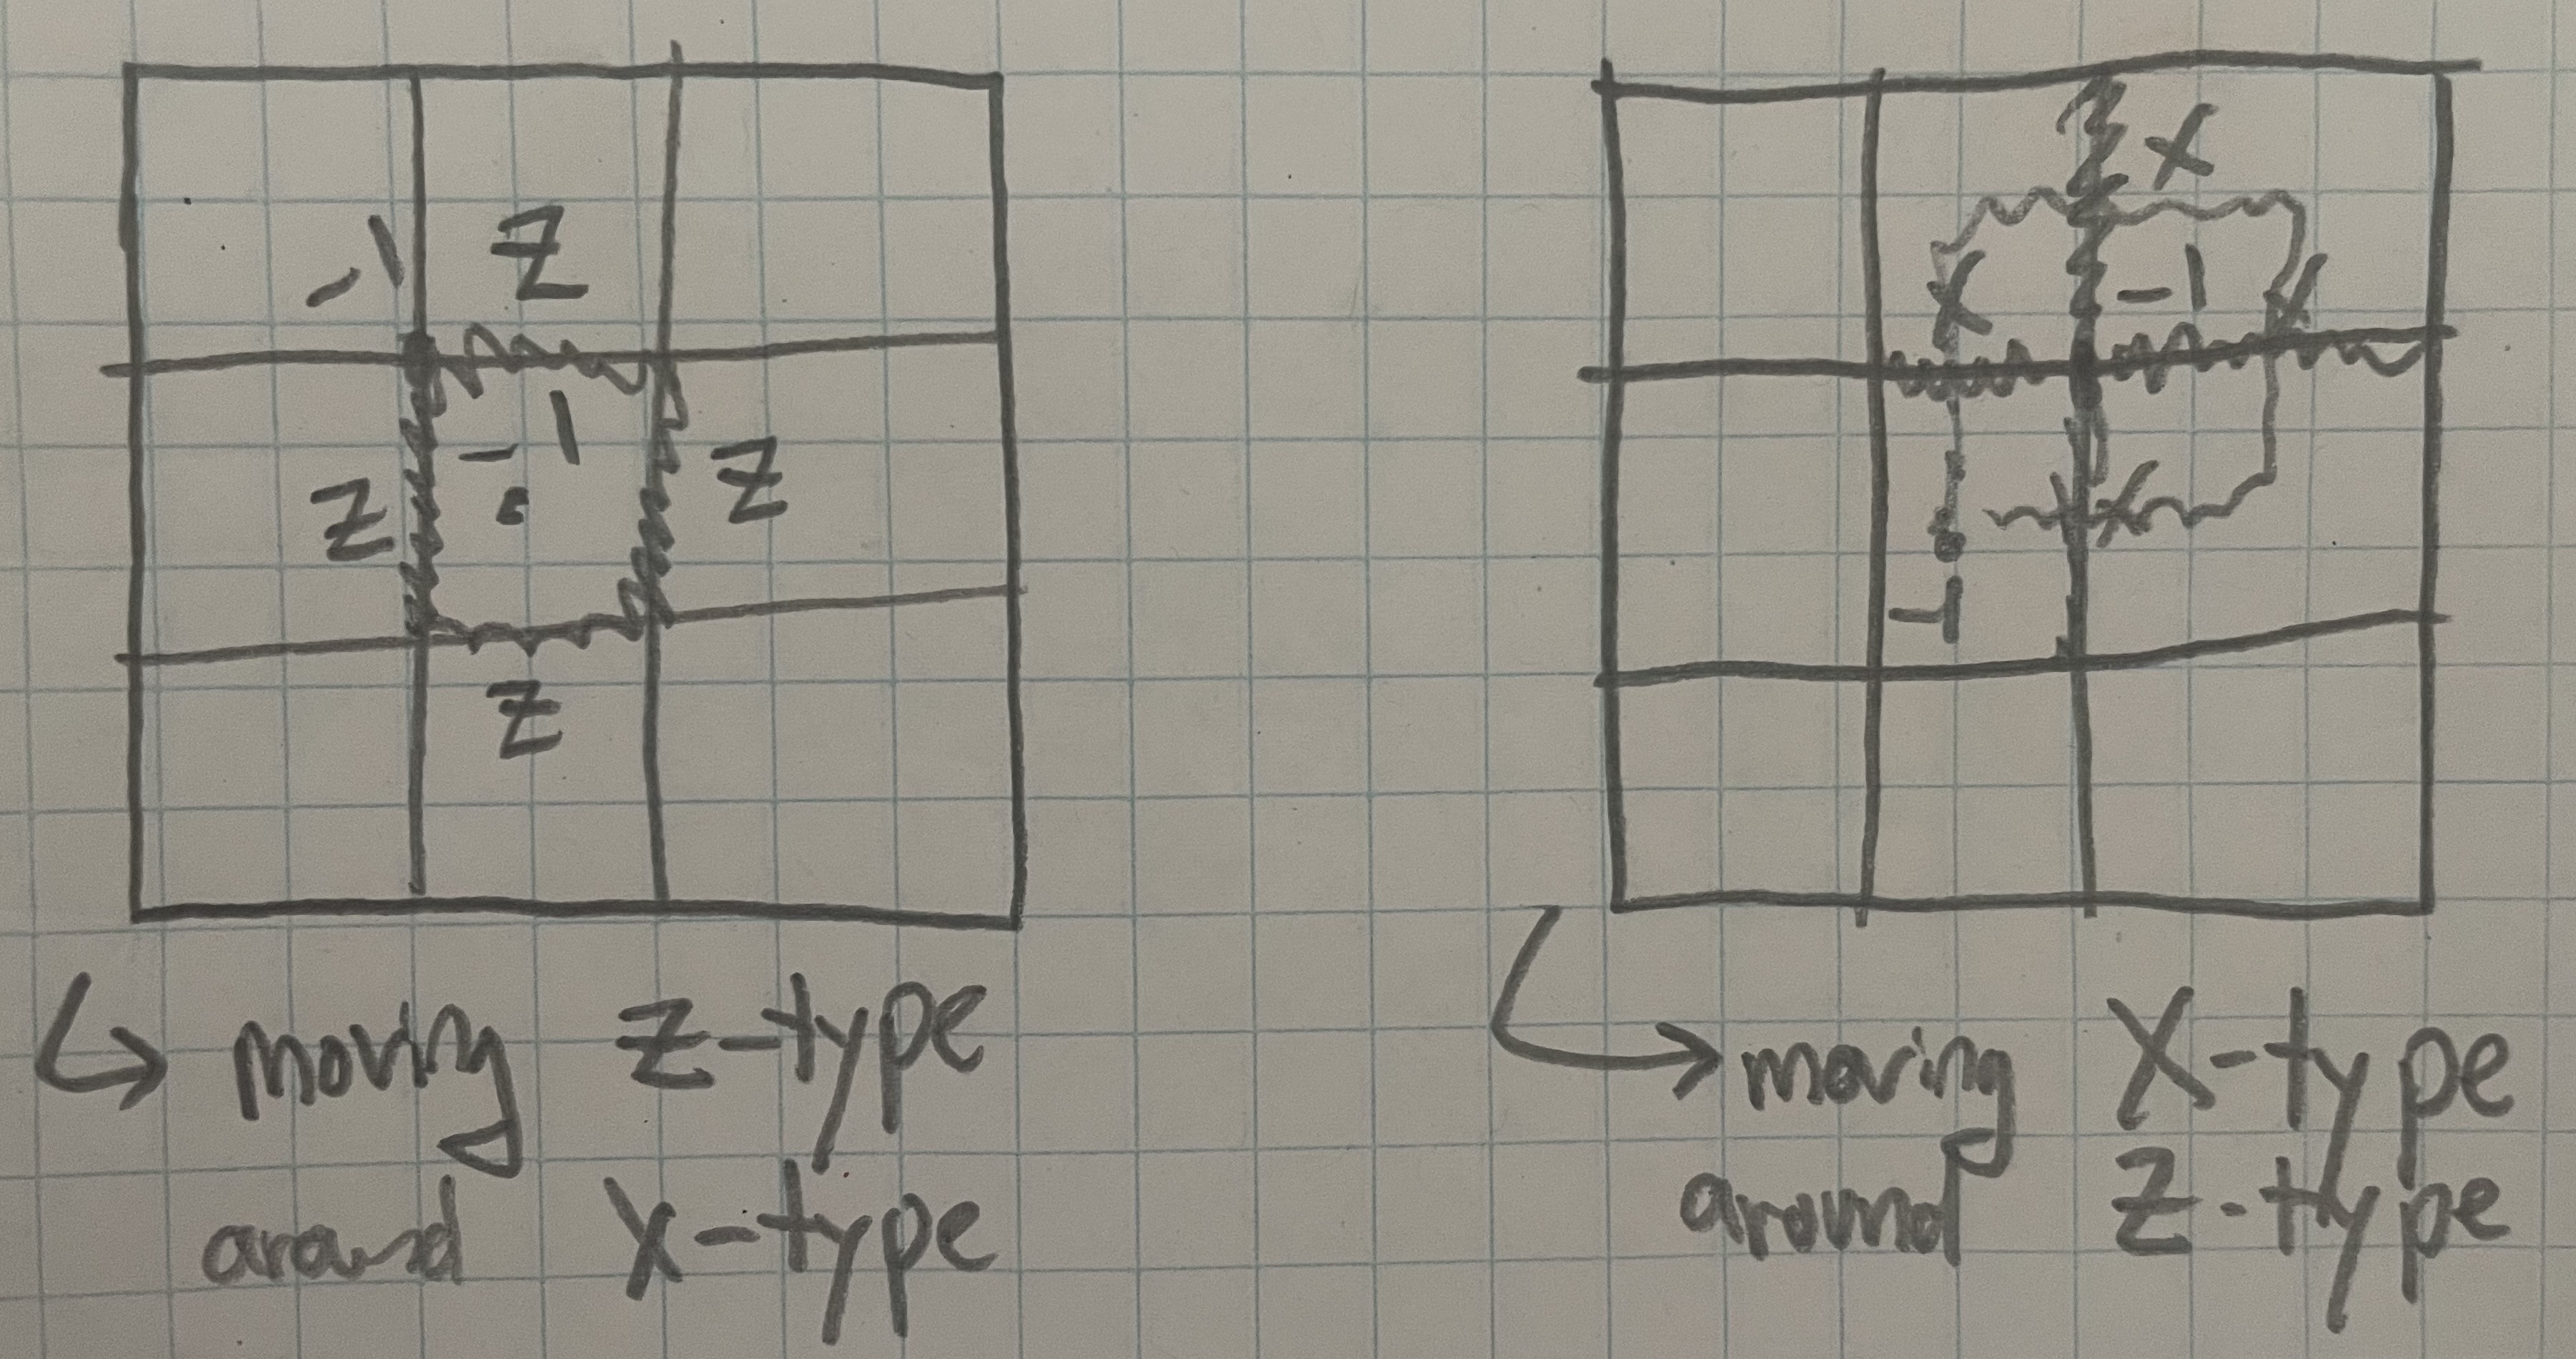
\includegraphics[scale=.04]{mutual-anyon-stats}
\end{center}
\end{figure}

We codify this in a proposition. However, seeing as we have not defined what it means for one anyon to move ``around" another, we can only state it on the physical level of rigor:

\begin{propositionph} Moving $X$-type anyons around $Z$-type anyons results in a phase of $-1$. Similarly, moving $Z$-type anyons around $X$-type anyons results in a phase of $-1$.
\end{propositionph}
\begin{proof}.[WORK: do proof]
\end{proof}

There is also an interesting action of anyons on the ground states of the toric code. This action is performed by starting with a ground state, creating anyon pairs, and then moving one of the anyons in that pair around a non-trivial loop around the torus, and then annhilating it back with its partner. This process is shown below:

[WORK: include diagram]

We can describe this action completely as fllows:

[WORK: give the picture of TQC by moving anyons around in proposition-format]

This concludes our picture of anyons in the toric code.

\subsection{Non-abelian anyons}

\subsubsection{Principles of anyons}

We recall that \textit{anyons} are localized excitations in topologically ordered systems. They behave as quasiparticles. In the previous section we analysed the toric code, and explored the behavior of anyons in the toric code. There were two types of anyons : $X$-type and $Z$-type. Each anyon type was its own antiparticle. The anyons braided trivially with themselves, but bothing any type of anyon around the other results in a $-1$ phase. In this subsection we will discuss the general theory of anyons which the toric code is part of.

To begin, we will recall some broader themes in particle physics. The modern world of particle physics is dominated by the \textit{standard model}. This model is a quantum field theory which describes the fundamental particles of the universe and how they interact. There are 61 different elementary particle types, each taking part in a broad explanation of the fundamental forces of the unvierse. An important feature of the standard model is a dichotemy between \textit{bosons} and \textit{fermions}. When bosons are exchanged it does not affect their underlying wave function, and when fermions are exchanged it results in a phase of $-1$.

Put more concretely, consider some particle type $A$. Let $V_2$ denote the Hilbert space of a system containing $2$ identical $A$-type particles. We can consider a unitary operator $\swap:V_2\to V_2$, which encodes the action on $V_2$ induces by taking the two particles and swapping their positions. It is a feature of the standard model that the details of how this swap doesn't change the action on $V_2$ - there is a well-defined $\swap$ map which only depends on the topology of the swap. It is a fact from the standard model that either $\swap$ is the identity map or $\swap$ is the unitary which multiples phases by $-1$. If $\swap=I$ then we call $A$ a boson, and if $\swap=-I$ we call $A$ a fermion.

We now explain why all of the particles in the standard model are bosons or fermions. The general idea is as follos. If we swap twice, then the particles go back to their original position. Hence, $\swap^2=I$. Hence, $\swap=I$ or $\swap=-1$. This general arguments works well for the standard model, but it has several subtleties which are important to highlight. Firstly, just because $\swap^2$ brings the particles got back where they started doesn't mean that the path they took has trivial topology. In space time it looks like the following:

\begin{figure}[h]
\begin{center}
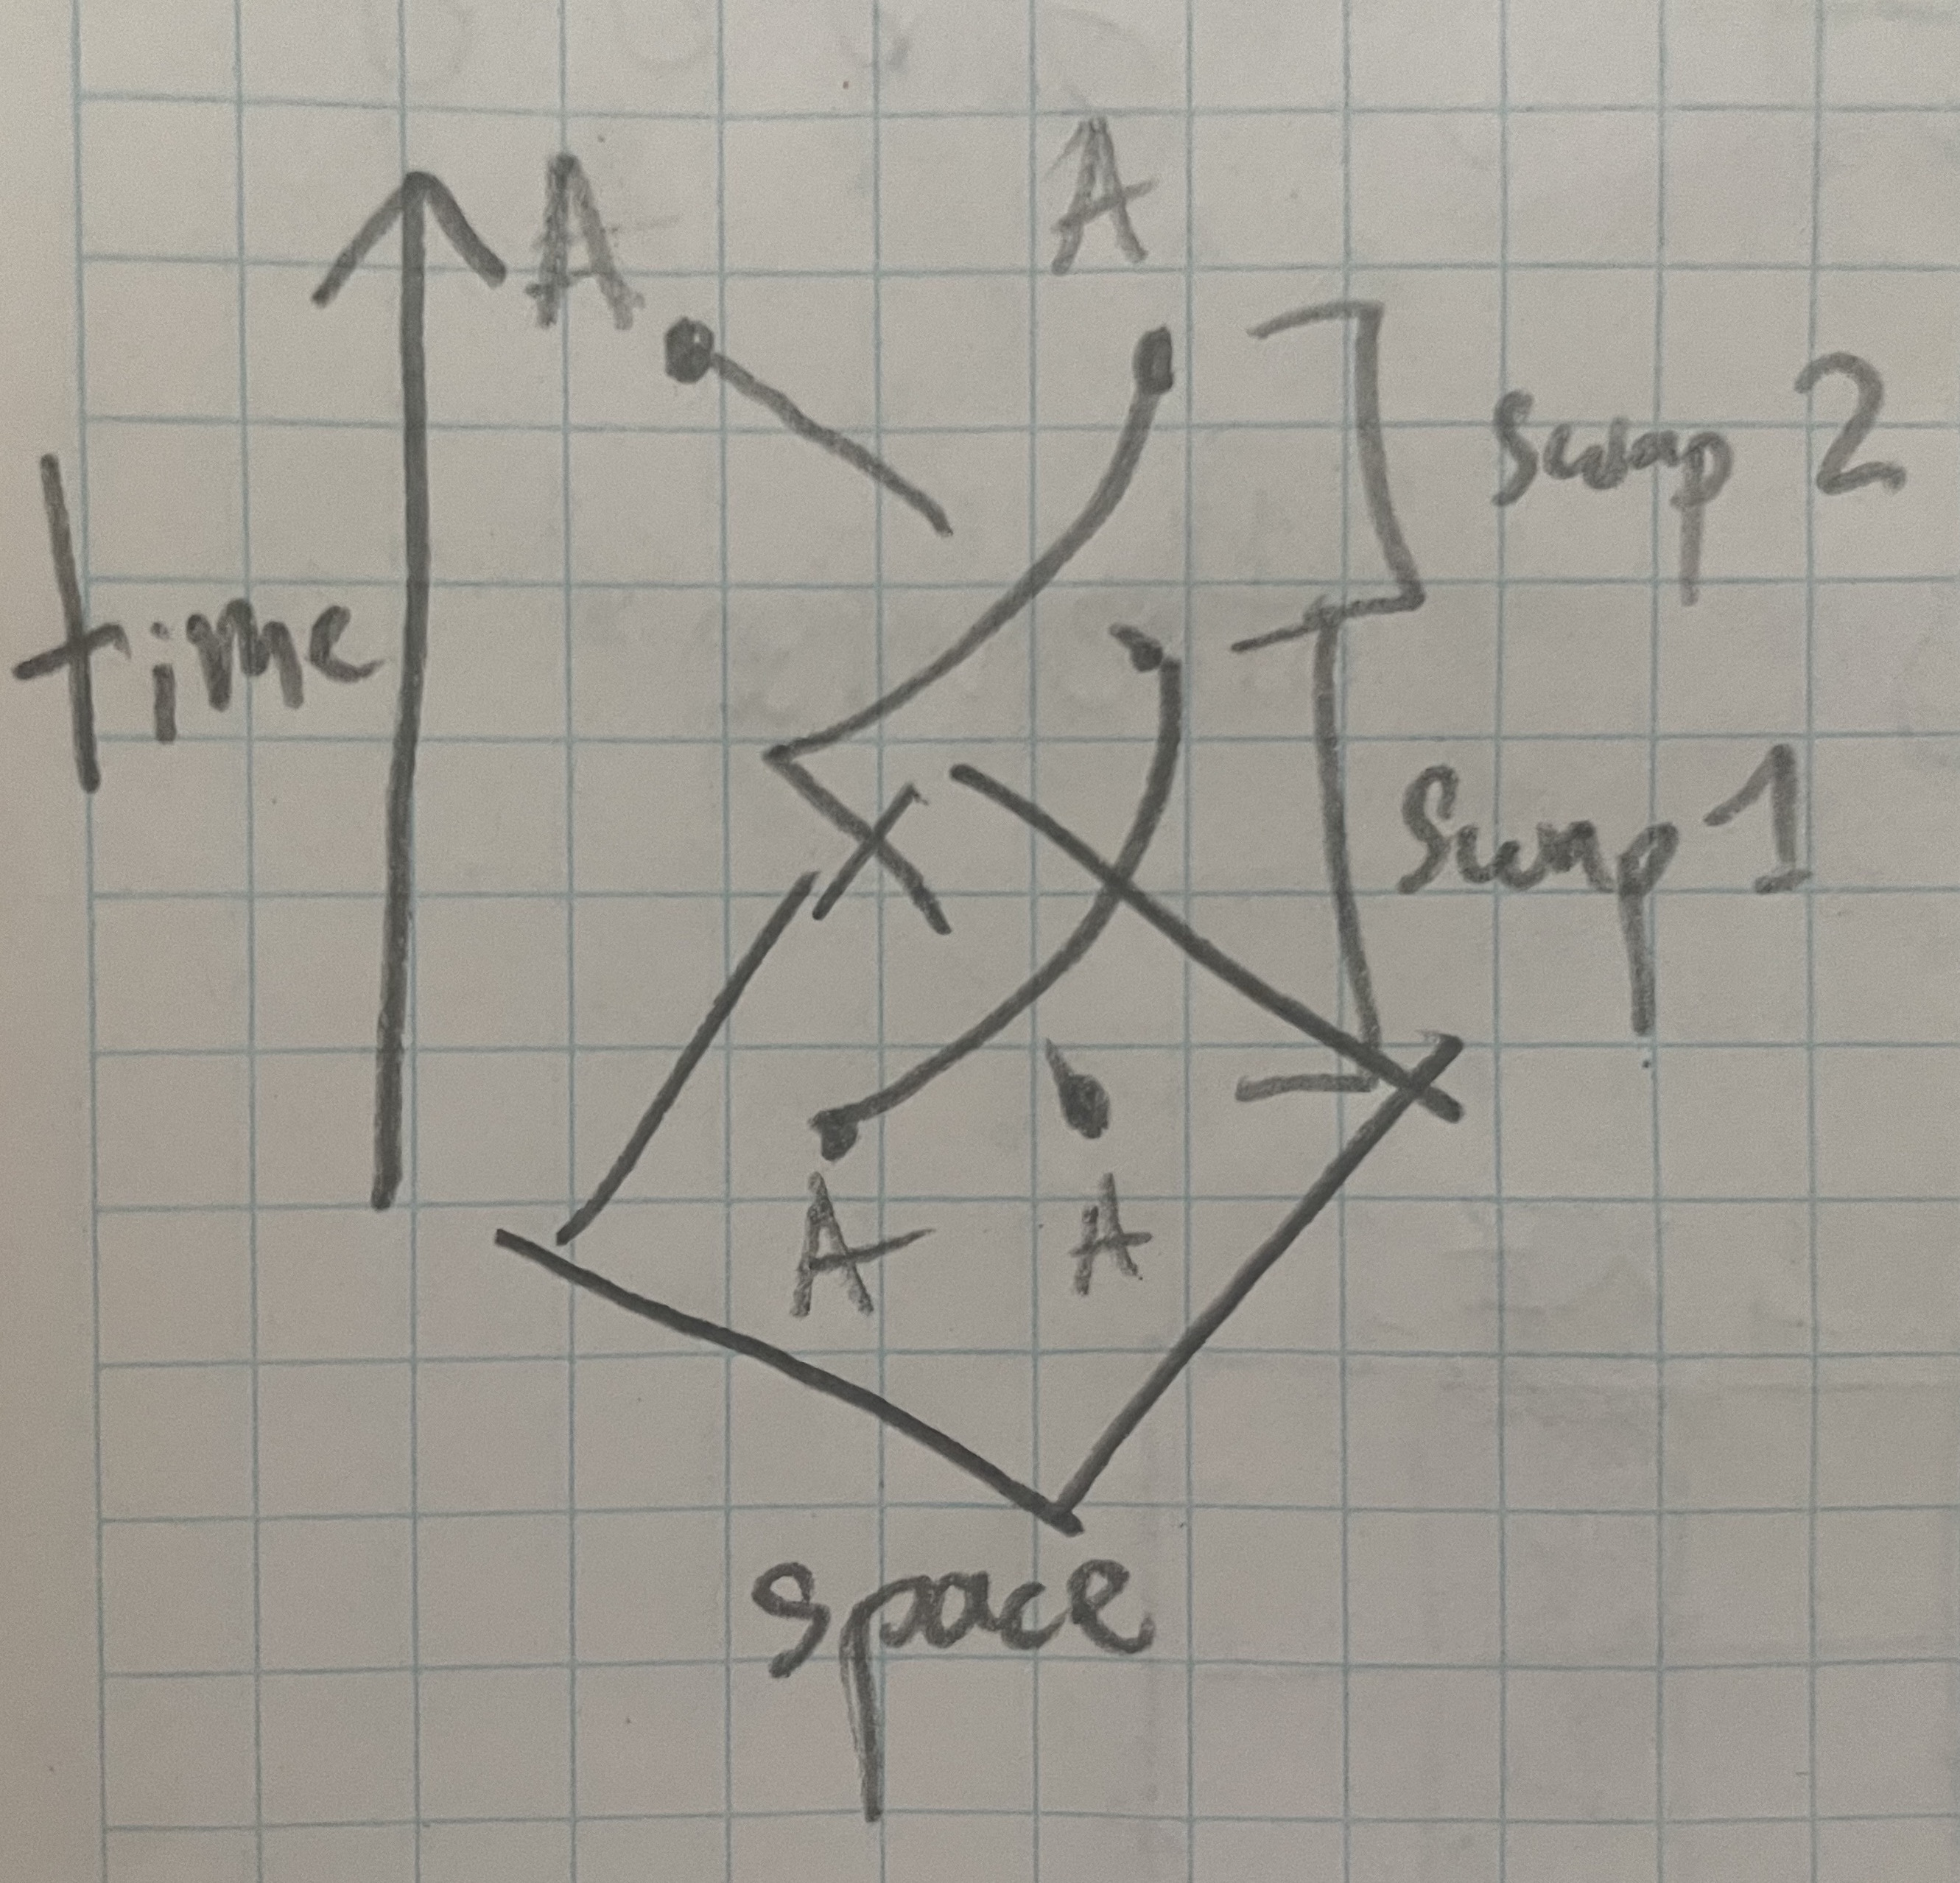
\includegraphics[scale=.04]{two-swaps}
\end{center}
\end{figure}

If physical space had two dimensions, then this is a topologically nontrivial braid. The important feature of the standard model is that it has three space dimensions. In three space dimensions, the double swap has trivial topology: the two strands can be moved smoothly past each other without intersected by pushing them into different parts of the third dimension. In general, the possible ways that $n$ particles can move around each other in two dimensions is the braid group $B_n$ we defined in section [ref], whereas the ways that particles can move around each other in three dimensions degenerates to the symmetric group $S_n$. Let $V_n$ denote the $n$ particle system of $n$ identical particles of type $A$. In two dimensions, moving the $n$ particles around in braids gives a representation

$$B_n\xrightarrow{}U(V_n)$$

whereas in three dimensions it gives a representation

$$S_n\xrightarrow{}U(V_n).$$

This difference between $B_n$ and $S_n$ causes a huge change between what is possible in three dimensions versus two dimensions. For instance, suppose that our braids only act by phases. That is, the image of the particle statistics maps lie in $U(1)\hookrightarrow{}U(V_n)$. In $B_n$, there is such a representation corresponding to any phase $\omega\in U(1)$. In this representation, exchanging two identical particles results in a phase $\omega$. In $S_n$, there are only two such representations: the trivial representation and the sign representation, corresponding to the phases $+1$ and $-1$ accordingly. These two representations correspond to bosons and fermions.

The last part of the explanation of why all particles in the standard model are fermions and bosons is more subtle. From our above discussion, it is clearly a-priori possible that there could be particles in 3 spacial dimensions which act by non-trivial higher dimensional representations of $S_n$. It turns out that this doesn't happen, and in fact it \textit{can't} happen in any (3+1)D quantum field theory, but this is for much more subtle reasons [WORK: add refs]. This doesn't mean that there aren't any models in 3 dimensions with quasiparticles that aren't bosons or fermions - these certainly exist [WORK: add refs]. It just means that these models are more rare and require some amount of trickery. The fact that all fundamental particles in (3+1)D quantum field theories are fermions or bosons is one of the main reasons we are working with (2+1)D systems in this book.

The toric code already demonstrates how particles can behave in ways in (2+1)D which are impossible in (3+1)D. When an $X$-type particle is moved all the way around a $Z$-type particle it results in a phase of $-1$. Of course, in (3+1)D moving one particle all the way around another is topologically trivial and hence would have to result in a phase of $+1$.

It is from this discussion that the name \textit{anyon} arrises. Bosons have $+1$ exchange phases, fermions have $-1$ exchange phases. Anyons, excitations in topolgoically ordered systems, can have \textit{any} exchange phase. Hence, \textit{any}on. Additionally, there are many natural systems which exhibit anyons whose exchange statistics results in higher dimensional representations of the braid group. These are known as \textit{non-abelian} anyons. Anyons which act by phases are known as \textit{abelian} anyons.

One intuition for the name abelian versus non-abelian comes from the Kitaev quantum double model. We will see that the Kitaev quantum double model based on a finite group $G$ hosts non-abelian anyons if and only if $G$ is non-abelian. Alternatively, you could motivate the name by noticing that an anyon is abelian if and only if the image of its associated braid group representation is abelian.

The algebraic theory of anyons is the heart and soul of topological order. This is quantified by the fact that our algebraic description of topological order will really be an algebraic description of anyons, and we will be asserting implicitely that describing the behavior of the anyons is enough to describe the topological order.

\subsubsection{The $G=D_4$ Kitaev quantum double model}

.[WORK: I'm assuming that this is the easiest model to work with. There should be nice descriptions for the line operators, and there should be a nice way of getting useful information out. Maybe its better to do stuff for general $G$? This is something that will require a lot of care to do right.]

$\newline$
\fbox{\parbox{\dimexpr\linewidth-2\fboxsep-2\fboxrule\relax}{

\begin{center}
\textbf{History and further reading:}\\
\end{center}

The term topological order was first used in 1972 by Kosterlitz and Thouless to describe topological classical systems of the sort discussed in Chapter [ref] \cite{kosterlitz2018ordering} . The term has since evolved, and was re-coined in 1989 by Xiao-Gang Wen to describe the sort of topological classical systems defined in this chapter \cite{wen1989vacuum}.

$\newline$
The history anyons is distinct from the history of topological order. It was first noted in 1976  in a paper of Leinass and Myrheim that the classification of particles in terms of fermions and bosons broke down in two dimensions \cite{leinaas1977theory}. The subject of anyons was then taken over by Wilczek who published a series of seminal papers on the topic \cite{wilczek1982magnetic, wilczek1982quantum, arovas1984fractional}. It was in these papers that Wilczek observed that anyons were present in the quantum Hall effect, and hence connected the theory of anyons and topological order together.

[WORK: what is the history of gauge theory, and when was it introduced to the picture? A great reference is the de Wild Propitius and Bais survey. Also should mention Kitaev's paper again.]

}}


$\newline\newline$

\large \textbf{Exercises}:\normalsize

\begin{enumerate}[\thesection .1.]

\item For vertices $v$ and plaquettes $p$, define

\begin{align*}
A'_{v,1}=\bigotimes_{\substack{\text{edges} \\ \text{touching }v}}\sigma_Z, && A'_v=\frac{1}{2}\left(I + A'_{v,1}\right),
\end{align*}

\begin{align*}
B'_{p,1}=\bigotimes_{\substack{\text{edges} \\ \text{bounding }p}}\sigma_X, && B'_p=\frac{1}{2}\left(I + B'_{p,1}\right),
\end{align*}

and

$$H'=\sum_{\text{vertices }v}(1-A'_v)+\sum_{\text{plaquettes }p}(1-B'_p).$$

Define $M:\CC^2\to \CC^2$ by $M(\ket{0})=\frac{1}{\sqrt{2}}(\ket{0}+\ket{1})$ and $M(\ket{1})=\frac{1}{\sqrt{2}}(\ket{0}-\ket{1})$. Show that

$$\sigma_X=M\sigma_ZM^{-1},\,\, \sigma_{Z}=M\sigma_X M^{-1},$$

and show that $H$ and $H'$ are similar in the sense that $H'=MHM^{-1}$. Use this to conclude that all basis independent properties of the toric code are formally symmetric by replacing $\sigma_X$ with $\sigma_Z$. For example, conclude that the codespace of $H'$ is 4 dimensional.

\end{enumerate}

\section{Category theory}

\subsection{Overview}

\subsubsection{Introduction}

There is a lot of math in the world. The development of the subject has spanned thousands of years, and has enjoyed a large uptick in the last two hundred or so. This has given ample time for the most important ideas to rise to the top. Among these important concepts there is one which is the focus of chapter: \textbf{composition}.

Let $A,B,C$ be sets. Let $f:A\to B$ and $g:B\to C$ be functions. The \textit{composition} of $f$ and $g$ is the function $g\circ f: A\to C$ defined by the formula $(g\circ f)(x)=g(f(x))$ for all $x\in A$. More generally, composition is the act of doing one process followed by a second process. Composition is distinguished in its importance for two reasons:

\begin{enumerate}
\item Composition is ubiquitous;
\item A very large number of more complicated structures can be described in terms of composition.
\end{enumerate}

These two primary reasons of importance lead to several emergent applications of composition:

\begin{enumerate}
\item It's a good organization principle - thinking in terms of composition gives a unifed approach to disperate subjects, which highlights the universality latent within mathematics;
\item It's a good compression technique - in a composition-forward approach there's no need to remember details about objects or functions between them, only the way that those functions compose is used;
\item Sometimes composition rules are the only data we have, making a composition-forward technique the only approach possible.
\end{enumerate}

This third point is the situation we find ourselves in with tthe algebraic theory of topological quantum information. We're trying to give a usable mathematical description of topologically ordered systems. The way that we find ourselves doing this is by focusing on anyons (the local quasiparticle excitations in topological order). Doing this we run into three important ponts:

\begin{enumerate}
\item Describing anyons exactly is hard. They are emergent phenomina, found within highly-entangled energy eigenstates of arbitrarily complicated gapped Hamiltonians.
\item Describing the possible ways that anyons can transform is hard. This involved specifying intricate unitary operators on high-dimensional Hilbert spaces.
\item Describing the ways that these transformations compose with one another is always relatively simple. It can be done using explicit-to-describe rules, which are independent of system size or choice of gapped Hamiltonian.
\end{enumerate}

What to do in this situation is clear: we will take a composition-first approach to anyons.

We give some examples to demonstrate our point. Suppose we want to discuss braiding anyons in the toric code. We can abstractly talk about a syndrome of the toric code in which there is one $X$-type particle and one $Z$-type particle:

[WORK: write out state.]

On these states we can talk about braiding. We use the same sorts of spactime diagrams as before to represent these transformations:

[WORK: write out state.]

Without talking about the fact that transformations of this type are realized explicitely using Pauli operators, we can still abstractly discuss the way they compose with each other:

[WORK: write out composition line]

[WORK: add more complicated example coming from whatever case of Kitaev quantum double I describe explicitely in the TO chapter]

The mathematical objects which allows one to speak intelligently about composition-first appraoches is known as a \textit{category}. The composition-first approach to mathematics is known as \textit{category theory}. Of course, to describe anyons we will need more than just the structure of composition. We will also need a way to encode what happens we we put anyons together, braid them, and fuse them. There structures are all completely compatible with the compostion-first approach, and correspond to adding extra structures onto the category. The categories describing anyons will all their extra structures is known as a \textit{modular tensor category}, and will be the subject of much of this book. This chapter deals with introducing category theory, as well as some of the structures which will be important for discussing anyons and modular tensor categories.

\subsubsection{Definition and important obervations}

As discussed before, a category is the structure which allows for a composition-first approach to map. Before going forward lets give a formal definition of category:

\begin{definition}[Category] A category is the following data:

\begin{enumerate}
\item (Objects) A set $\C$.
\item (Morphisms) A set $\Hom(A,B)$ for all $A,B\in \C$
\item (Composition) Functions

$$\circ: \Hom(B,C)\times \Hom(A,B)\to \Hom(A,C)$$

for all $A,B,C\in \C$.
\end{enumerate}

Such that:

\begin{enumerate}

\item $(h\circ g)\circ f = h\circ (g\circ f)$, for all morphisms $f\in \Hom(A,B)$, $g\in \Hom(B,C)$, $h\in\Hom(C,D)$,  and objects $A,B,C,D\in \C$.

\item (Identity) For all objects $A\in \C$ there exists a morphism $\id_{A}: A\to A$ such that for all $B\in \C$, $f\in \Hom(A,B)$, and $g\in \Hom(B,A)$,

\begin{align*}
f\circ \id_{A}=f, && \id_{A}\circ g = g.
\end{align*}

\end{enumerate}

\raggedleft\qedsymbol{}
\end{definition}

The rest of this section will contain a loosely-related series of five observations about this definition:

$\newline$
\textbf{Observation 1:} \textit{The structure of this definition is very typical of algebra.}

Roughly, algebra is defined to be the study of algebraic structures. An algebraic structure, roughly, is defined to be some collection structures on some space, with rules outlining how the structures interact with each other. The general way of definding algebraic structures is to first list the structures, and then list the axioms of how these structures inteact with each other. We will see many definitions of this sort throughout the rest of the book, so it is good to get used to it now.

$\newline$
\textbf{Observation 2:} \textit{In this text we have already seen many examples of categories.}

We list some of them below:

\begin{itemize}
\item $\Set$, the category of sets. The objects are sets and the morphisms are functions.

\item $\mathbf{Top}$, the category of topological spaces. The objects are topological spaces and the morphisms are continuous functions.

\item $\mathbf{Vec}_k$, the category of finite dimensional vector spaces over a field $k$. The objects are finite dimensional vector spaces over $k$ and the morphisms are linear operators.

\item $\mathbf{Grp}$, the category of finite groups. The objects are finite groups and the morphisms are group homomorphisms.

\item $\mathbf{Hilb}$, the category of quantum systems. The objects are finite dimensional Hilbert spaces and the morphisms are unitary operators.

\item $\mathbf{Prob}$, the category of probability spaces. The objects are finite dimensional real vector spaces with distinguished bases and the morphisms are operators which send normalized vectors to normalized vectors.

\item $\mathbf{Ord}_M$, the category of ordered media with order space $M$. The objects are continuous maps $\phi: \RR^2\to M$ and the morphisms are continuous deformations.

\end{itemize}

$\newline$
\textbf{Observation 3:} \textit{The objects and morphisms of a category do not have much complexity implicit to them.  All of the interesting structure is encoded within the composition structure.}

This is despite the fact that when we listed our examples in Observation 2 we only described the objects and morphisms, and not the compositoin structure. The reason for this is that the composition structure between morphisms in all of our examples is clear. In all our examples the objects are sets with extra strcture, and the morphisms are maps of sets. The composition structure is inhereted from the composition structure on functions between sets.

Going further, however, we observe that objects in abstract categories are \textit{not} required to be sets and the morphisms are \textit{not} required to be functions of sets. Most of our examples of categories will have objects which are sets and morphisms which are functions of sets, but there will be notable counterexamples. It is important to remember that there are some categories for which there is no interpreation of morphisms as functions between sets \cite{freyd1970homotopy}.

$\newline$
\textbf{Observation 4:} \textit{A category isn't just a space with a good notion of composition - it also has identity maps.}

These identity maps are important, and we include them in the definition purposefully. There are two primary reasons: firstly that all of the relevant examples of categories will have identity maps, and secondly that most interesting properties of categories only make sense because of the identity maps. Hence if we didn't require identity maps then we would find ourselves constantly requiring them as a condition, which is a waste of space.

It is important to take a closer look at what the identity map means, though. The identity map is trying to capture a very general phenominon about transformations: \textit{there is always the trivial transformation which results from doing nothing}. This do-nothing map is the identity. In the category of sets, the identity maps on the set $A$ is given by the formula $\id_A(x)=x$ for all $x\in A$. The fact that these maps are the identities in the category of sets is the reason that the identity axiom for categories is defined like it is. Really, there is an implicit lemma hidden in the definition of category:

\begin{lemma} Let $A$ be a set. For all sets $B$ and for all $f:A\to B$, $g:B\to A$ we have

\begin{align*}
f\circ \id_{A}=f, && \id_{A}\circ g = g.
\end{align*}

In particular, $\id_A$ satisfies the axiom of an identity in the category of sets, and hence $\Set$ forms a category.
\end{lemma}
\begin{proof}.[WORK: do proof]
\end{proof}

These sorts of implicit lemmas are everywhere in category theory. Whenever a composition-forward definition is given in category theory, there is the assumption that it agrees with the standard definition at least in the category of sets. For instance, we make the following definition:

\begin{definition}[Isomorphism] Let $\C$ be a category, let $A,B\in C$ be objects, and let $f:A\to B$ be a morphism. We say that $f$ is an \textit{isomorphism} if there exists a morphism $f^{-1}:B\to A$ such that $f^{-1}\circ f= \id_A$ and $f\circ f^{-1}=\id_B$. We call $f^{-1}$ the \textit{inverse} of $f$. In this case, we say that $A$ and $B$ are \textit{isomorphic objects}.

\raggedleft\qedsymbol{}
\end{definition}

The implicit lemma in this definition is as follows:

\begin{lemma} Let $A,B$ be sets, and let $f:A\to B$ be a function. The map $f$ is a bijection if and only if there exists a function $f^{-1}: B\to A$ such that $f^{-1}\circ f= \id_A$ and $f\circ f^{-1}=\id_B$. In particular, a function $f$ in the category $\Set$ is an isomorphism if and only it is a bijection.
\end{lemma}
\begin{proof}.[WORK: do proof]
\end{proof}

$\newline$
\textbf{Observation 5:} \textit{Statements in category theory can be very broadly applied.}

This is in some sense obvious by the fact that there are so many different examples of categories, but it's good to state the observation explicitely. Here's a good example:

\begin{proposition} Let $\C$ be a category. Identities in $\C$ are unique. Explicitely, let $A\in \C$ be an object and let $\id_A,\tilde{\id}_A:A\to A$ be morphisms satisfying the identity axiom. We have that $\id_A=\tilde{\id}_A$.
\end{proposition}
\begin{proof}. Using the fact that $\id_A \circ f = f$ and $f\circ \tilde{\id}_A=f$ for any $f:A\to A$, we compute that

$$\id_A= \id_A \circ \tilde{\id}_A = \tilde{\id}_A$$

as desired.
\end{proof}

This has broad application. For instance: why are identity elements in groups unique? Le $G$ be a group and let $1,1'\in G$ be identity elements. We find that $1=1\cdot 1' = 1'$ as desired. Going further, here is another proposition in category theory:

\begin{proposition}
\label{inverse-unique}
Let $\C$ be a category. Let $A,B$ be objects and let $f:A\to B$ be an isomorphism. The inverse of $f$ is unique. That is, let $f^{-1},\tilde{f}^-1$ be morphisms satisfying the definition of the inverse of $f$. We have that $f^{-1}=\tilde{f}^{-1}$.
\end{proposition}
\begin{proof} Using the associativity axiom, we compute

$$f^{-1}=f^{-1}\circ \id _{B} = f^{-1}\circ (f \circ \tilde{f}^{-1})=(f^{-1}\circ f)\circ \tilde{f}^{-1}=\id_A \circ \tilde{f}^{-1}=\tilde{f}^{-1}$$

as desired.
\end{proof}

This is very general. Why are inverses unique in groups? Why are inverses of matrices unique? Abstractly, why should the inverse of any reversible process be unique? Proposition \ref{inverse-unique} gives the answer.

\subsection{Structures in category theory}

[WORK: this section should include all of the structures which are neccecary for the rest of the book,
and are too cumbersome to define on-site. It should also read as an introducting to how to think in the language of categories. Here is the running list of neccecary topics

\begin{itemize}
\item Products/coproducts/biproducts
\item $\CC$-linear structure
\item Functors, natural equivalence, equivalence of categories, NOT Yoneda lemma
\end{itemize}
]

[WORK: maybe use homotopy theory as a reccuring motivating example?]

\subsection{Monoidal categories}

[WORK: should work the reader up to comfort-level with monoidal categories. Hard to write without knowing what is in the structures in category theory section.]

[WORK: Needs BRAIDED monoidal categories and RIGID monoidal categories. Maybe two different subsections. This should be done using left-rigid, right-rigid. It makes sense to then talk about them together, as pivotal categories, and prove the two equivalent characterization of pivotal categories.]

[WORK: needs to introduce and make use of diagramatic notation for monoidal categories.]

$\newline$
\fbox{\parbox{\dimexpr\linewidth-2\fboxsep-2\fboxrule\relax}{

\begin{center}
\textbf{History and further reading:}\\
\end{center}

Category theory was first introduced and formalized by Saunders Mac Lane and Samuel Eilenberg in 1945 \cite{eilenberg1945general}. Of course, the ideas underlying category theory were present earlier and can be traced back arbitrarily far. In the subsequent decades the formalism of category theory spread far and wide, bringing with it the discovery of many deep theorems. The first major explicit appearance of category theory in physics was Vladimir Drinfeld's work on so-called \textit{quantum groups} in the early 1980s \cite{drinfeld1986quantum}. Quantum groups are certain kinds of mathematical objects righly related to content in this book. They were introduced as tools to help generate exactly-solvable models in condensed matter physics. Very quickly quantum groups were absorbed into the theory of the ideas of string theory of topological quantum field theory, which were both new at the time \cite{belavin1984infinite, witten1988topological}. The physics in this area has since become and remained extremely categorical in nature \cite{lurie2008classification, bartlett2015modular}.

$\newline$
There are many excellent introductory texts to category theory. Some authors find it fruitful to reformulate all of quantum mechanics, and especially quantum information, in terms of category theory. A good source outlining this approach and introducing category theory through it is Coecke-Kissinger's textbook \cite{coecke2018picturing}. The Kong-Zhang textbook \cite{kong2022invitation} gives an introduction to category theory in the context of topological order. A good general-purpose textbook on category theory is Fong-Spivak \cite{fong2019invitation}, and a classical but slightly dated reference is \cite{mac2013categories}.
}}


$\newline\newline$

\large \textbf{Exercises}:\normalsize

\begin{enumerate}[\thesection .1.]

\item .[WORK: make exercises]

\end{enumerate}

\section{Modular tensor categories}

\subsection{Overview}

\subsubsection{Introduction}

In this chapter we will be giving a detailed analysis of modular tensor categories, the abstract algebraic structures used to describe anyons in topological order. We recall below how this fits into the general framework of this book:

[WORK: add diagram]

Describing exactly what an anyon and how it can transform in terms of states and unitary operators on a Hilbert space can be difficult. However, describing abstractly how these transformations compose with one another can be done realtively simply. Hence we take a composition-first category-theoretic approach to anyons. We will make heavy use of the diagramatic language of braided monoidal categories established in Chapter [ref]. More concretely, we will think of a modular tensor category as being the category with the following data:

\begin{equation*}
\left(\substack{
\mathbf{objects:}\text{ finite collections of anyons}\\
\mathbf{morphisms:}\text{ motions/behaviors of anyons}
}\right)
\end{equation*}

Up to topological equivalence, there are not that many things that a collection of anyons can do. The most basic thing is to move anyons around each other - this is known as braiding. If the anyons touch each other then they can congeal into a single composite anyon - this is known as fusion. Even if there are no anyons in a system, however, there is always something possible. Anyons can be spontaneously created, so long as every anyon which is created comes along with its corresponding antiparticle. This is known as \textit{pair-creation}. These three operations are the fundamental structures which we will building into modular tensor categories:

\begin{enumerate}
\item braiding;
\item fusion;
\item pair-creation.
\end{enumerate}

One potentially useful way of thinking about modular tensor categories comes from analogy with classical physics. We saw in Chapter [ref] that topological classical systems have an algebraic description in terms of finite groups. Namely, quasiparticles in the system of ordered media with order space $M$ is algebraically characterized by the fundamental group $\pi_1(M,m)$ of $M$ relative to some basepoint $m\in M$. Seeing as topological order is a vast quantum generalization of classical ordered media, we can think of modular tensor categories as being a vast quantum generalization of finite groups. Every finite group induces a modular tensor category, by first constructing the Kitaev quantum double model based on that finite group and then describing its anyons. Most modular tensor categories, however, lie beyond this description.

Due to the frequency of our use of the term, we will abbreviate modular tensor category to \textit{MTC}.

\subsubsection{Using the final product}

Before developping the theory of modular tensor categories (MTCs), it is good to get a feel for what using the final product is like. An MTC itself will be a big infinite thing, with infinitely many objects and infinitely many morphisms between those objects. However, all MTCs are in a real sense \textit{finitely generated}. What we mean by this is that plugging in a finite number of objects and morphisms, the rest of the obejcts and morphisms can be recovered by the abstract rules encoded in the formalism. For example, consider the 3-strand braid group $B_3$. This group has ininitely many elements and the group operation $\cdot: B_3\times B_3\to B_3$ takes a-priori an infinite amount of data to describe. However, the presentation

$$B_3=\Braket{\sigma_1, \sigma_2 | \sigma_1 \sigma_2 \sigma_1 = \sigma_2 \sigma_1 \sigma_2}$$

gives  completely finite description of $B_3$. It is important to note, however, that this presentation would \textit{not} have been enough to recover $B_3$ if we had just been told that $B_3$ is a monoid. The fact that $B_3$ is a group implied the existence of elements $\sigma_1^{-1}$, $\sigma_{2}^{-1}$, and defined how they interacted with $\sigma_1,\sigma_2$. We see in this way that the axioms of a group not only serve as a restriction on what mathematical objects are allowed to be groups, but they also serve as a compression technique. They give the rules by which a minimal collection of data can be used to generate the rest.

In a similar way, the axioms of MTCs are not only neccecary by the fact that they restrict which categories can be MTCs, but they are also vital in the fact that they allow us to generate a full description of anyons from a minimal collection of data. For practically-minded readers, this can be viewed as the main motivation for defining MTCs at all, instead of just working with important examples.

The final challenge in going from MTCs to their description in terms of a finite set of data is in comming up with an efficient standard way of descrbing morphisms in an MTC. This is done using the Yoneda perspective, as discussed in section [ref].

In the end, the data of an MTC will look like what we have below for the toric code:

[WORK: add toric code MTC data]

Or, for a more complicated example, we can consider the data for $G=S_3$:

[WORK: add $G=S_3$ MTC data]

A large table of these descriptions are found in Chapter [ref]. We now give a worked example of how this data is used to compute observable quantities.

[WORK: add good example, computing some probability of annhilation]

\subsection{First properties}

\subsubsection{Definition}

In this section we finally define modular tensor categories (MTCs), which are the main mathematical content of this book. Seeing as lots of data is involved, we spread out the definition over a series of steps as to not overload the senses. These intermediate definitions are also important in their own right, because they will be used in other places in the algebraic theory of topological phases.


\begin{definition}[Fusion category] A fusion category is the following data:

\begin{enumerate}
\item A category $\C$;
\item The structure of a right-rigid monoidal category on $\C$;
\item The structure of a $\CC$-linear category on $\C$.
\end{enumerate}

Such that:

\begin{enumerate}
\item The tensor product functor $\otimes: \C\times \C\to \C$ induces bilinear maps hom-spaces;
\item There is an equivalence $\C \cong \Vec_\CC^n$ as $\CC$-linear categories;
\item $\End_\C(\one)\cong \CC$ as $\CC$-vector spaces
\end{enumerate}

\raggedleft\qedsymbol{}
\end{definition}

A fusion category is part of the way towards having all of the requisite structures of a modular tensor category: it has a method for fusion inherited from the tensor product, and it has half of a method for pair-creation coming from right-rigidity. The $\CC$-linearity allows us to think of hom-spaces as vector spaces, which allows us to treat hom-spaces as quantum systems. The condition (1) is a comptability between the $\CC$-linear structure and the monoidal structure. The conditions (2)-(3) are strong niceness and finiteness conditions - we will explain them in detail later. We now move one step closer to our definition of modular tensor category:

\begin{definition}[Spherical fusion category] A spherical fusion category is the following data:

\begin{enumerate}
\item A spherical category $\C$;
\item A left-rigid structure on $\C$.
\end{enumerate}

Such that:

\begin{enumerate}
\item The left-rigid and right-rigid structures on $\C$ satisfy the axioms of a pivotal structure on $\C$;
\item For every object $A\in \C$ and for every morphism $f: A \to A$, we have

[WORK: add spherical diagram.]
\end{enumerate}

\raggedleft\qedsymbol{}
\end{definition}

A spherical fusion category now has a structure for fusion, and a full structure for pair-creation. The 2nd condition is known as the \textit{spherical axiom}. We will explain this axiom in more detail later.

Adding on a braiding, we can get all of the structures of a modular tensor category. However, adding this structure still misses one key structure of being a modular tensor category. Hence, we call it \textit{pre-modular}:

\begin{definition}[Pre-modular tensor category] A pre-modular tensor category is the following data:

\begin{enumerate}
\item A spherical fusion category $\C$;
\item A braided structure on $\C$;
\end{enumerate}

Such that:

\begin{enumerate}
\item .[WORK: compatibility between braiding + $\CC$-linearity, or compatibility between braiding and rigidity?]
\end{enumerate}

\raggedleft\qedsymbol{}
\end{definition}

This definition now has all of the structure we wanted it to have: fusion, pair-creation, and braiding. The final axiom is a non-degeneracy condition. It is subtle in its interpretation, and we will explain it several different ways throughout this chapter:


\begin{definition}[Modular tensor category] A modular tensor category is a pre-modular tensor category satisfying the following condition:

[WORK: add condition]

\raggedleft\qedsymbol{}
\end{definition}


\subsubsection{Anyons in MTCs}

Modular tensor categories (MTCs) are supposed to be theories of anyons in topological order. So, now that we have the definition of MTC, it is natural to ask: what do anyons mathematically correspond to, in MTCs? The answer lies within the condition in a fusion category $\C$ that there is an equivalence $\C\cong \Vec_\CC^n$ as $\CC$-linear categories. We explore the importance of this condition.

Suppose we are given an object $V=(V_1,V_2...V_n)\in \Vec_\CC^n$. For all $1\leq i\leq n$, let  $\CC_i\in \Vec_\CC^n$ denote the object which has dimension zero in every index $j\neq i$ and is equal to $\CC$ in index $i$. We observe the isomorphism

\begin{align*}
V& \cong \bigoplus_{i=1}^n (0... V_i ... 0)\\
& \cong \bigoplus_{i=1}^n (0... \CC^{\dim (V_i)}.. 0)\\
& \cong \bigoplus_{i=1}^n \dim(V_i)\cdot \CC_i
\end{align*}

where $\dim(V_i)\cdot (\CC_i)=\CC_i\oplus \CC_i...\oplus \CC_i$, $\dim(V_i)$ many times. This computation shows that any object in $\Vec_\CC^n$ can be decomposed into irriducible components $\CC_i$. These objects $\CC_i$ are in a real sense the building blocks of $\Vec_\CC^n$. They will correspond physically to anyons. More concretely, we make the following definition:

\begin{definition} A \textit{simple object} $A$ in a fusion category $\C$ is an object which has no direct sum decomposition into smaller objects. That is, $A\ncong B\oplus C$ for any non-zero objects $B,C\in \C$ where $\oplus$ denotes the biproduct in $\C$.
\end{definition}

Our physics-math dictionary is that anyon types correspond to isomorphism classes of simple objects.

We now state the basic proposition which ensures that the neccecary properties from $\Vec_\CC^n$ follow through the equivalence of categories.

\begin{proposition} Let $\C$ be a fusion category. The biproduct of any two elements in $\C$ exists. Let $\LL$ denote the set of isomorphism classes of simple objects in $\C$. The set $\LL$ is finite. Choose an object $X\in \C$. There exist unique nonnegative integers $c_{[A]}$, $[A]\in \LL$ such that 

$$X\cong \bigoplus_{[A]\in \LL}N_{[A]}\cdot A.$$
\end{proposition}
\begin{proof}.[WORK: do proof.]
\end{proof}

The set of simple objects has an alternative description, known as Schur's lemma:

\begin{proposition}[Schur's Lemma] Let $\C$ be a fusion category. An object $A\in \C$ is simple if and only if its endomorphism ring $\End(A)$ is one-dimensional. Additionally, if $A,B\in \C$ are nonisomorphic simple objects then $\Hom(A,B)=0$.
\end{proposition}
\begin{proof}.[WORK: do proof.]
\end{proof}

As an immediate application of Schur's lemma, we observe that the monoidal unit $\one$ is a simple object in every fusion category. By our physics-math dictionary, this means that $\one$ corresponds to an anyon type. This type is the \textit{vaccuum} type - empty space. The anyon $\one$ is the trivial no-anyon type.

Another application of Schur's lemma is to make a first verification that simple objects are a good choice of mathematical characterization of anyons. If $A,B$ are distinct anyon types, then there should not be any physical process which goes from one to another. There is no physical mechanism for locally turning one anyon type into another. This is captured by the formula $\Hom(A,B)=0$. Similarly, given an anyon $A$, there is no nontrivial action that can be locally performed on $A$. This comes from the fact that information is topologically protected, and thus cannot be changed by acting on a single particle - topological information processing requires global braiding between multiple particles. This is encoded in the fact that $\Hom(A,A)\cong \CC$ is one dimensional and hence consists only of trivial phase gates.

Expanding our physics-math dictionary, we say that for every anyon $A$ its \textit{antiparticle} is the dual $A^*$ which comes from right-rigidity. This gives a valid anyon type by the following computation:

\begin{proposition} Let $\C$ be a fusion category. If $A\in \C$ is a simple object, then so is $A^*$.
\end{proposition}
\begin{proof}. [WORK: do proof]
\end{proof}

An important part of of understanding simple objects in MTCs is making sense of the direct sum decompositions coming from Proposition [ref]. Let $\C$ be a fusion category with simple objects $A,B\in \C$. Consider the decomposition

$$A\otimes B \cong \bigoplus_{[C]\in \LL}N^{A,B}_{C}\cdot C$$

where $N^{A,B}_{C}\geq 0$ are nonnegative integers, and $\LL$ is the set of isomorphism classes of simple objects. The integers $\{N^{A,B}_C\}_{[C]\in \LL}$ are known as fusion coefficents, because they specify the behavior of $A$ and $B$ when they fuse.

The tensor product $\otimes$ physically corresponds to joining anyons, forming a composite anyon configuration. The object $A\otimes B$ corresponds to the configuration with one $A$-type anyon and one $B$-type anyon. The direct sum decomposition is physically interpreted as saying that when $A\otimes B$ are fused, the possible results of that fusion are all of the anyon types $[C]\in \LL$ for which $N^{A,B}_{C}\neq 0$.

[WORK: add nontrivial example from Kitaev quantum double model]

A more detailed understanding of the physical meaning of the direct sum will have to wait for later.

This concludes our basic picture of anyons in fusion categories.

\subsubsection{States in MTCs and unitarity}

It is now worth reflecting on what exactly states correspond to in MTCs. In particular, objects in MTCs are \textit{not} quantum systems. They don't have vector space structure. The spaces with vector space structure are the hom-spaces, by $\CC$-linearity. Objects will correspond to anyon configurations. States will correspond to normalized vectors in certain hom-spaces. In particular:

\begin{equation*}
\left(\substack{\text{space of states of topological order $\C$} \\ \text{on the infinite plane $\RR^2$} \\ \text{with anyon configuraiton $A_1,A_2...A _n$}}\right)
=
\left(
\substack{
\text{normalized vectors in the Hilbert space}\\
\Hom_\C(\one, A_1\otimes A_2... \otimes A_n)
}
\right)
\end{equation*}

where by ``anyon configuration $A_1,A_2...A_n$" we mean that the state has anyons present in $n$ sites, arranged left to right on a one dimensional subspace of $\RR^2$, with corresponding anyon type $A_1,A_2...A_n$. For the sake of concreteness, one can imagine that at the point $(i,0)\in \RR^2$ thee state has an anyon of type $A_i$.

The remainder of this subsection is a series of loosely-related observations about this choice of state space:

$\newline$
\textbf{Observation 1:} \textit{In the definition of an MTC hom-spaces are vector spaces and not Hilbert spaces, so this choice of physics-math correspondance is incorrect as literally written}.

To make this definition work, all of the hom-spaces of the MTC $\C$ should be equipped with Hilbert space structures. Furthermore, the natural operators we wish to perform like braiding should all be unitary with respect to these inner products. This amounts to adding a large number of compatibility conditions on the Hilbert space structures. An MTC with this choice of structure is known as a \textit{unitary} MTC. We give the formal definition below:

\begin{definition}[Unitary modular tensor category] A unitary modular tensor category is the following data:

\begin{enumerate}
\item An MTC $\C$.
\item (Conjugation) A linear map $\dagger: \Hom(A,B)\to \Hom(B,A)$ for all $A,B\in \C$.
\end{enumerate}

Additionally, a unitary Modular Tensor Category is required to satisfy the following properties:

\begin{enumerate}
\item .[WORK: add properties]
\end{enumerate}

\raggedleft\qedsymbol{}
\end{definition}

For this reason, the correct algebraic structure to underlie the theory of topological order is not MTC, but unitary MTC. We have chosen to not emphasize this before because the difference between unitary MTCs and non-unitary MTCs is very small. [WORK: talk about uniqueness + positive q.d. criterion this will make more sense once we write the actual section about unitarity. A good thing to emphaize is that unitary MTCs don't let you use less data in your definition, and you can still do essentially everything you want to do. It's just way more cumbersome. They're all equivalent but you still have to choose, c.f. the fact that the category of vector spaces and Hilbert spaces with linear maps as morphisms are equivallent].

$\newline$
\textbf{Observation 2:} \textit{The physical space is assumed to be an infinitely large flat plane.}

The reason that the physical space is the infinitely large flat plane is that it has a unique ground state, and does not have boundaries. Finite contractible regions would have boundaries to worry about, and spaces with topology like the torus would have non-equivalent ground states. The formula $\Hom(\one,\one)\cong \CC$ implies that there is a unique ground state, whence the conclusion.

Describing anyons on spaces with non-trivial topology is a more difficult question, and requires more machinery [WORK: reference something later? Will I talk about this? Seems important.] 

$\newline$
\textbf{Observation 3:} \textit{The anyons are always assumed to be arranged in a line.}

The anyon configurations are always assumed to be linear. The main reason to do this is because it makes the mathematics much simpler. If we kept track of the positions of each of the anyons in two dimensional space it would add more pieces of data and structures to keep track of. Seeing as every anyon configuration can be pushed onto a one-dimensional space, only working with a one-dimensional configuration does not affect the generality of the answers and hence it is very much prefered.

$\newline$
\textbf{Observation 4:} \textit{The formula $\Hom_{\C}(\one, A_1\otimes A_2...\otimes A_n)$ encodes the fact that states can be specified by their history.}

A good first question to ask when seeing the Hilbert space $\Hom_\C(\one, A_1\otimes A_2... A_n)$ is \textit{why} this should describe a state with anyon configuration $A_1$... $A_n$. The answer is that states can be described their history. [WORK: give good example of making a state by specifying its history; argue why it has to be this way in general].

\subsubsection{Topological charge measurement}

When two anyons are fused together, they will form a superposition of other anyon types. Measuring the result of the fusion will collapse the answer into a specific anyon type. The outcome of this measurment is an observable quantity, which allows for the measurement of topological quantum information. In many cases this is the \textit{only} local observable quanitity. We give the formalism behind computing these probabilities now.

[WORK: do this right - I don't know it well but it shouln't be hard to learn. Don't introduce anything too general, like trace or whatnot. Just quantum dimension, which should already have been introduced in previous chapter.] 


\subsection{The MTC toolkit}

\subsubsection{Trace}

In this section, we will introduce and prove the basic facts about the most important structures in the theory of modular tensor categories (MTCs). These facts and structures can be viewed as tools, which are used for solving problems about the algebraic theory of anyons. 

 -
\subsubsection{Duality}

\subsubsection{Quantum dimension}

Our next tool to discuss is the \textit{quantum dimension}. Given any fusion category $\C$ and any simple object $A\in \C$, we define its quantum dimension using the following formula:

[WORK: define $d_A$.]

Upon first definition, $d_A$ is a morphism $\one\to \one$ in $\C$. By the axioms of a fusion category, $\End_\C(\one)\cong \CC$. Moreover, this isomorphism is canonical. That is, we can identity these two spaces via the unique linear map
$\End_\C(\one)\to \CC$ which sends $\id_{\one}\in \End_{\C}(\one)$ to $1\in \CC$. In this way, we can identity $d_A$ with a complex number.

\subsubsection{Twist}

\subsubsection{Verlinde formula}

\subsubsection{Functors, natural transformations, and equivalence}

\subsubsection{Deligne tensor product}



\subsection{Quantum double MTCs}

\subsubsection{The Drinfeld center}

\subsubsection{Muger's theorem}

\subsubsection{Levin-Wen model}

\subsubsection{Mortia equivalence}

\subsubsection{Factorizability}

\subsubsection{Quantum doubles of finite groups}



\subsection{The modular representation}

\subsubsection{Definition}

\subsubsection{Torus perspective}

\subsubsection{Proof of modularity}

\subsubsection{Proof of unitarity}

\subsubsection{Bruguieres's modularity theorem}

\subsubsection{Schauenberg-Ng theorem}



\subsection{The Yoneda perspective}

\subsubsection{Principle}

\subsubsection{$F$-symbols}

\subsubsection{$R$-symbols}

\subsubsection{$\theta$-symbols}

\subsubsection{Reconstruction theorem}



\subsection{Unitarity}

\subsubsection{Characterization of unitarizable MTCs}

\subsubsection{Uniqueness of unitary structure}

\subsubsection{Yoneda perspective on unitarity}




\subsection{Number theory in MTCs}

\subsubsection{.[prerequisites and introduction]}

\subsubsection{Galois conjugation}

\subsubsection{Ocneanu rigidity}

\subsubsection{Rank-finiteness theorem}

\subsubsection{Vafa's theorem}

.[WORK: this section is going to host a lot more theorems]




\subsection{Adjectives in MTCs}

\subsubsection{Solvability}

\subsubsection{Nilpotence}

.[WORK: surely more adjectives will be hosted here.]


$\newline$
\fbox{\parbox{\dimexpr\linewidth-2\fboxsep-2\fboxrule\relax}{

\begin{center}
\textbf{History and further reading:}\\
\end{center}

Modular tensor categories were born from conformal field theory in the late 1980s. In a series of papers, Moore and Seiberg analysed deeply the underlying content within conformal field theory to find what essential algebraic data lied within it \cite{moore1988polynomial, moore1989classical}. They wrote out the axioms of this essential algebraic data in their subsequent notes on conformal field theory \cite{moore1990lectures}. They used the name modular tensor category to describe their data, as suggested by Igor Frenkel. This definition was then refined and re-introduced by Turaev \cite{turaev1992modular}. The first major application of modular tensor categories was the Reshetikhin-Turaev construction \cite{reshetikhin1991invariants, turaev2010quantum}. Prior to this result nobody had succeed in constructing topological quantum field theories. In this way, modular tensor categories and the Reshetikhin-Turaev construction completed Witten's programme of quantizing Chern-Simons theory.

$\newline$
By the early 2000s, the proposal of topological quantum computing was attracting a lot of interest in anyons and their algebraic properties. Seeing as topological order can be described by topological quantum field theory and topological quantum field theory is essentially equivalent to modular tensor categories, it was understood that modular tensor categories could be used to understand topological order. This latent description of anyons in terms of modular tensor categories was made explicit in an appendix in the seminal 2006 paper of Kitaev \cite{kitaev2006anyons}. This approach to anyons in terms of modular tensor categories was popularized by Wang's early monograph \cite{wang2010topological}. This has since become the standard approach towards the algebraic theory of topological quantum information.
}}


$\newline\newline$

\large \textbf{Exercises}:\normalsize

\begin{enumerate}[\thesection .1.]

\item .[WORK: apply Verlinde formula to group-theoretical MTCs to recover classical theorem by Burnside]

\end{enumerate}


\section{Further structure}

\subsection{Overview}

\subsection{Domain walls}

\subsection{Symmetry enriched topological order}

\subsection{Fermionic topological order}


$\newline$
\fbox{\parbox{\dimexpr\linewidth-2\fboxsep-2\fboxrule\relax}{

\begin{center}
\textbf{History and further reading:}\\
\end{center}

[WORK: add history]
}}


$\newline\newline$

\large \textbf{Exercises}:\normalsize

\begin{enumerate}[\thesection .1.]

\item .[WORK: make exercises]

\end{enumerate}

\section{Topological quantum computation}

\subsection{Overview}

\subsubsection{Introduction}

In this section we will discuss topological quantum computing, the concept of making a computer based on topological quantum systems. We recall now ow this fits into the overall framework of this book:

[WORK: add diagram]

We recall some general principles and motivations for topological quantum computing, most of which were outlined in Chapter [ref]. Seeing as we will be making repeated use of the term, we abbreviate topological quantum computing to \textit{TQC}.

The most important idea in the subject is that TQC is inherently \textit{fault tolerant}. Noise in the environment of a quantum computer, when properly controlled, can be made small in magniude and local in effect. By the definition of a topological system, the information in the topological computer is invariant under small local changes. Hence, the information remains invariant under noise and the computation can proceed as intended without errors. If there are errors, which is always possible with some small probability, topological quantum systems typically have mechanisms whereby the experimenter can remove the error and restore the information how it was. This is the general picture for fault tolerance in TQC. We will make this picture more precise as we give examples of methods for TQC.

We additionally recall that TQC splits into two major branches. The first is the method of finding physical materials that naturally exhibit topological quantum behavior. These systems can then be used to make a computer. The second approach is to simulate a topological quantum system on a quantum computer. This simulation is used to inheret the fault-tolerant properties of the topological quantum systems on the original quantum computer. So long as the simulation is efficient and local noise on the physical system corresponds to local noise on the simulated system, this method works as described. This gives the following diagram for TQC:

[WORK: add diagram - its already used somewhere else!]

In this chapter, we will talk about lots of different approaches to TQC. Some of them are naturally ammenable to the approach of topological quantum materials, and some of them are naturally ammenable to the approach of topological quantum error correction. We will flag these differences and the status of experimental progress as we go along.

Before moving on with our discussion of TQC, it is good to be aware of the limitations of the algebraic approach.

\begin{enumerate}
\item Introducing the algebraic theory is a lot of overhead for not very many examples. Overwhelmingly, proposals for TQC center around just a few algebraic models. Topological quantum error correction is mostly centered around the toric code (see section [ref]), and topological quantum materials are mostly centered around Majorana fermions (see section [ref]). The vast majority of algebraic models have no serious proposals for TQC associated with them. It is for this reason that much of the literature is focused on working out the details of small models and examples, instead of the development of general theory which is largely useless in this lens.

\item The algebraic structures fail to capture a lot of important details about proposals for TQC. It only captures the high-level information flow, and none of the microscopic features. For example, a breakthrough in the field of topological quantum error correction come with the introduction of \textit{color codes} in 2006 \cite{bombin2006topological}. These color codes have very nice properties, and have been an important player in the field of TQC. However, algebraically the color code is equivalent to bilayer toric code:

$$(\text{color code})\cong (\text{toric code})\boxtimes (\text{toric code}).$$

The entirely of the novelty of the color code comes in its specific choice of Hamiltonian and microscopic details - there is no new algebra involved.

\end{enumerate}

All this is not to say that the algebraic theory of topological quantum information is useless. It has been an important guide in the subject, and has provided footing and motivation for the continued development of TQC. Large-scale fault-tolerant quantum computation is one of the defining technological challenges of the 21st century. It seems very likely that topological methods will be part of its realization!

\subsubsection{Universality}

An important concept for understanding TQC methodology is \textit{universality}. To illustrate this concept we begin with an example.

In 1994, Peter Shor developped an efficient quantum algorithm for factoring integers \cite{shor1994algorithms}. This algorithm is important because much of modern cryptography is based on the hardness of factoring integers and similar problems. Hence, an efficient factoring algorithm could jeapordize internet security.

However, we must pose ourselves the question: what does it mean, really, for Shor to have found an efficient quantum factoring algorithm? A quantum computer is a computer whose information processing is fundamentally described by quantum mechanics. A priori there are lots of different quantum computers one could make. Which one did Shor find a factoring algorithm for? Maybe when we finally make a quantum computer it will be the type of quantum computer which cannot run Shor's algorithm so internet security will be safe.

The key in understanding this situation is the concept of universality. There are certainly quantum computers which cannot run Shor's algorithm. For instance, if a quantum computer has only a finite number of degrees of freedom to store information then it certainly cannot run large cases of Shor's algorithm because it can't even record the input! Even if a quantum computer can store arbitrarily large inputs, that doesn't mean it will have the capabilities to run Shor's algorithm because it might just not have a physical method for running the algorithm.

However, every \textit{sufficiently powerful} quantum computer can run Shor's algorithm. Moreover, every algorithm you can run efficiently can run efficiently on one quantum computer can then be run on every other sufficiently powerful quantum computer.

Here is the explination for this phenominon. Computers can be viewed as simulation devices. Quantum computers are simultation devices which can simulate quantum systems. Suppose that you are given two quantum computers $\text{QC}1$ and $\text{QC}2$. If $\text{QC}1$ is sufficiently powerful, it should be able to efficienlty simulate the behavior of $\text{QC}2$. If $\text{QC}2$ is sufficiently powerful, it should be able to efficiently simulate the behavior of $\text{QC}1$, as illustrate below:

\[\begin{tikzcd}
	{\text{QC}1} && {\text{QC}2}
	\arrow["{\text{efficient simulation}}", curve={height=-12pt}, from=1-1, to=1-3]
	\arrow["{\text{efficient simulation}}", curve={height=-12pt}, from=1-3, to=1-1]
\end{tikzcd}\]

This gives an easy way to turn any efficient algorithm on $\text{QC}1$ into an efficient algorithm on $\text{QC}2$. First you simulate $\text{QC}1$, and then you run the algorithm on $\text{QC}1$! This means that any problem solved on one of the computers can be efficiently solved on the other. In this way these two computers are \textit{computationally equivalent}. The non-trivial inisght is that every sufficiently powerful quantum computer is able to efficiently simulate every other sufficiently powerful quantum computer. These powerful quantum computers which can simulate every other computer are known as \textit{universal} quantum computers. The existence of universal quantum computers is the heart of universality. What Shor did was make a factoring algorithm which could be run on any universal quantum computer.

This sort of universality has been known for a long time. It was first proposed by pioneers of computation Alan Turing and Alonzo Church \cite{turing1939systems, copeland1997church}:

\begin{quote}
Church-Turing thesis: ``All sufficiently powerful computational models yield efficiently intersimulable classes - there is one theory of computation".
\end{quote}

Of course, this thesis does not account for the possibility of quantum computation. Classical and quantum computation seem to be turly distinct theories of computation, violating Church-Turing's intention. This leads to a modern revised version of the Church-Turing thesis:

\begin{quote}
Revised Church-Turing thesis: ``All sufficiently powerful classical computational models yield efficiently intersimulable classes - there is one theory of classical computation".
\end{quote}

A quantum version of the Church-Turing thesis was introduced in an early review article on topological quantum computation by Michael Freedman, Alexei Kitaev, Michael Larsen, and Zhenghan Wang \cite{freedman2003topological}. It goes as follows:

\begin{quote}
Freedman-Church-Turing thesis: ``All sufficiently powerful computational models which add the resources of quantum mechanics to classical computation yield efficiently intersimulable classes - there is one theory of quantum computation".
\end{quote}


The goal, then, is to make a \textit{universal} topological quantum computer. In a sense this makes designing a scheme for topological quantum computation difficult. It gives constraints, and forces a certain amount of computation power. In another sense, it is liberating. The existence of universal quantum computation means that once we have implemendent a certain amount of computational power into our proposal, we are done. There is no need to search for clever ways to add more power because or system is already universal, and hence finding more techniques in unnececary. It gives an end goal to building a quantum computer - a bell to ring when we are done.

[WORK: there is the general corrolation between computational power, difficulty of implimentation, and non-abelian flavor. Give the nice table and talk about it.]





\subsection{Computational complexity}

\subsubsection{Principles}

The revised Church-Turing and Freedman-Church-Turing theses state that there is one theory of classical computation and one theory of quantum computation. This leads to a very natural question: \textit{what are those theories?} These theories are mathematically codified as computational complexity classes. They are named as follows:

\begin{align*}
\text{(Efficient clasical computation)} &= \P = ``\text{polynomial time}",\\ 
\text{(Efficient quantum computaiton)} & = \BQP = ``\text{bounded-error quantum polynomial time}."
\end{align*}

The computational class $\BQP$ inherently has randomness built into it, because quantum mechanics inherently has randomness built into it. The ``bounded-error" in $\BQP$ refers to the fact that quantum computations will have some probability of error because they are probabilistic. A tool we will use to help define and understand $\BQP$ is the intermediary computational class associated with classical computers that have randomness built into their architecture:

$$\text{(Efficient probabilistic computaiton)}  = \BPP = ``\text{bounded-error probabilistic polynomial time}".$$

As a first application of these complexity classes, we can start to make more precise statements about the nature of quantum computaion. For instance, we may ask the following question: \textit{does the power of quantum computation come from its ability to harness randomness?} The answer is \textbf{no}, conjecturally. We formalize this as follows. We first observe that give more recourses to a computer can only expand the number of efficient algorithms:

\begin{proposition} $\P \subseteq \BPP \subseteq \BQP$.
\end{proposition}

We will prove this later, once we have formally defined $\P$, $\BPP$, and $\BQP$. We now state two widely belived conjectures:

\begin{conjecture}$\,$
\begin{enumerate}
\item $\P=\BPP$;
\item $\BPP \subsetneq \BQP.$
\end{enumerate}
\end{conjecture}


As a particular case, we can consider factoring. Shor proved that $(\text{factoring})\in \BQP$. Conjecturally, there are no efficient classical algorithms for factoring:

\begin{conjecture} $(\text{factoring})\not\in \P$.
\end{conjecture}

Proving conjectures [ref] is already quite difficult. In particular, it would resolve a millinium prize problem! The problem of factoring is known to live in a certain computational complexity class called $\NP$. Hence, we we know that factoring was in $\NP$ but factoring was not in $\P$ then we could conclude that $\P\neq \NP$. However, $\P\neq \NP$ is a millinium prize problem, and is very much unsolved. The general theme is that it is quite difficult to show that computaional complexity classes are distinct.

Every method for topological quantum computation induces a computational complexity class. It neccecitates a way of storing, manipulating, and reading out information. The ultimate goal of every chapter will be to prove that the method described is equivalent to $\BQP$, and hence gives a universal quantum computing scheme.

\subsubsection{Classical computation}

We will now formalize the theory of classical computation, with the end goal of defining the computational complexity class $\P$ of polynomial time algorithms. Of course, there are many different equivalent ways of formulating the theory of classical computation.The Church-Turing thesis says that all of these different ways will give the same final answer. The method we will use for formalizing information theory is the method of circuits.


We will store our information in \textit{bits}. These are classical objects with two element state spaces. We denote a bit abstractly as $\ZZ_2=\{0,1\}$. Computations are functions

$$f:\ZZ_2^n\to \ZZ_2^m$$

for some $n,m\geq 1$. The basic computations are \textit{logic gates}. We will work with the logic gates $\NOT$, $\AND$, and $\OR$. They are defined as follows:

\begin{align*}
\NOT: \ZZ_2&\xrightarrow{}\ZZ_2 && \AND: \ZZ_2^2\xrightarrow{}\ZZ_2 && \OR:\ZZ_2^2\xrightarrow{}\ZZ_2\\
0&\mapsto 1 && (1,1) \mapsto 1 && (1,1)\mapsto 1\\
1&\mapsto 0 && (1,0)\mapsto 0 && (1,0)\mapsto 1\\
& && (0,1)\mapsto 0 && (0,1)\mapsto 1\\
& && (0,0)\mapsto 0 && (0,0)\mapsto 0\\
\end{align*}

A depth-1 circuit is a map $f:\ZZ_2^n\to \ZZ_2^m$ such that each component of the output is either a constant, the same as one of the input components, or one of the basic logic gates $\NOT$, $\AND$, and $\OR$. For example, the map

\begin{align*}
f:\ZZ_2^4&\xrightarrow{} \ZZ_2^4\\
(b_1,b_2,b_3,b_4)&\mapsto (\AND(b_2,b_4), 0, b_1, \OR(b_1,b_3))
\end{align*}

is a depth-1 circuit. A depth-$k$ circuit is a map $f:\ZZ_2^n\to \ZZ_2^m$ which can be written as a composition on $k$ depth-1 circuits. Our intuitive notion of computational complexity is that a computation $f:\ZZ_2^n\to \ZZ_2^m$ is \textit{efficient} if it can be represented as a circuit which uses few logic gates. That is, the sum of the number of logic gates used in each of its layers is small. The most important feature of these circuits is that every computation can be expressed in terms of them:

\begin{proposition} Every function $f:\ZZ_2^n\to \ZZ_2^m$ for any $n,m\geq 1$ can be written as a circuit of some finite depth.
\end{proposition}
\begin{proof}.[WORK: add reference for proof]
\end{proof}


We define a \textit{classical decision problem} $F$ to be a sequence of functions

$$F=\left\{f_n: \ZZ_2^{n}\to \ZZ_2\right\}_{n=1}^{\infty}.$$

An \textit{algorithm} for a classical computation problem $F$ is a well-definiteness rule for writing circuits which equal each $f_n$.

\begin{definition}
We define $\P$ to be the set of all classical decision problems $F$ for which there exists a classical algorithm for $F$ such that there exists a polynomial $p(n)$ for which

$$\left(\substack{\text{\# of logic gates } \\ \text{in circuit for $f_n$}}\right)\leq p(n).$$

\raggedleft\qedsymbol{}
\end{definition}

This definition of $\P$ is not rigorous, because in the definition of algorithm we used the intuitive notion of a \textit{well-defined} process. Formalizing exactly what one means by a well-defined rule is subtle, and it is typically done using the language of Turing machines.

\subsubsection{Probabilistic computation}

We now formalize probabilistic computation in analogy to classical computaion. Bits can now be indeterminate - they have a probability of being 0 and a probability of being 1. Abstractly, this probabilistic bit is the real vector space $\RR[\ZZ_2]$. Computations are functions

$$f:\RR[\ZZ_2^n]\to \RR[\ZZ_2^m]$$

for some $n,m\geq 1$ which send normalized vectors to normalized vectors. Using the canonical isomorphism $\RR[S\times T]\cong \RR[S]\otimes \RR[T]$, we may also think of computations as maps

$$f:\RR[\ZZ_2]^{\otimes n}\to \RR[\ZZ_2]^{\otimes m}.$$

All of the classical logic gates $\NOT$, $\AND$, and $\OR$ naturally yield probabilistic logic gates by acing on the distinugished basis. A depth-1 circuit is defined exactly as before. It is a map $f:\RR[\ZZ_2^n]\to \RR[\ZZ_2^m]$ such that each component of the output is either constant, the same as one of the input components, or one of the basic logic codes $\NOT$, $\AND$, or $\OR$. The key difference is that in probabilistic computation there are more constants. For instance, the element $\frac{1}{4}\ket{0}+\frac{3}{4}\ket{1}$ is a constant in $\RR[\ZZ_2]$. The map

\begin{align*}
f:\RR[\ZZ_2]^{\otimes 3}&\xrightarrow{} \RR[\ZZ_2]^{\otimes 5}\\
b_1\otimes b_2\otimes b_3&\mapsto b_2\otimes \AND(b_1,b_2)\otimes \left(\frac{1}{2}\ket{0}+\frac{1}{2}\ket{1}\right)\otimes \NOT(b_3)\otimes b_1
\end{align*}

is an example of a depth-1 circuit. A depth-$k$ circuit is a map $f:\RR[\ZZ_2]^{\otimes n}\to \RR[\ZZ_2]^{\otimes m}$ which can be written as a composition of $k$ depth-1 cirucits. Again, this definition is well-chosen because it captures all possible computations:

\begin{proposition}. [WORK: not sure exactly what the correct statemenet is here.]
\end{proposition}

The subtelty in defining the computational class $\BPP$ is that it will \textit{not} have to do with probabilistic decision problems. $\BPP$ will consists of classical decision problems which have efficient probabilistic algorithms. Let $F=\{f_n\}_{n=1}^{\infty}$ be a classical decision problem. A probabilistic algorithm for $F$ is a well-defined rule for writing circuits $\tilde{f}_n:\RR[\ZZ_2]^{\otimes n}\to \RR[\ZZ_2]$ for each $n\geq 1$ such that for all $x\in \ZZ_2^n$

$$(\text{Probability that $\tilde{f}_n(\ket{x})=1$})=
\begin{cases}
\geq 2/3 & \text{if } f_n(x)=1,\\
\leq 1/3 & \text{if } f_n(x)=0.\\
\end{cases}$$

\begin{definition}
We define $\BPP$ to be the set of all classical decision problems $F$ for which there exists a probabilistic algorithm for $F$ such that there exists a polynomial $p(n)$ for which

$$\left(\substack{\text{\# of logic gates } \\ \text{in circuit for $\tilde{f}_i$}}\right)\leq p(n).$$

\raggedleft\qedsymbol{}
\end{definition}

The key point in this definition is that the probabilistic algorithm does not have to recover $f_n(x)$ exactly. It only has to do so approximately. The numbers $2/3$ and $1/3$ are chosen somewhat arbitrarily. The important point is that $2/3$ is strictly larger than $1/2$ and $1/3$ is strictly less than $1/2$. In this way, running the algorithm gives strictly better information than guessing randomly would. To get more accuracy, $\tilde{f}_n$ can be ran polynomially many times. The output of the computation can then be taken to be the majority outcome of the results of $\tilde{f}_n(\ket{x})$. Running $\tilde{f}_n$ increasingly many times gives an increasingly high probability of getting the right answer.

\subsubsection{Quantum computation}

We now formalize quantum computation in analogy to classical and probabilistic computation. Bits are now replaced with two level quantum systems. Abstractly, this quantum bit is the quantum system $\CC[\ZZ_2]$. We identity $\CC[\ZZ_2]$ with $\CC^2$ for convenience. We refer to the quantum bit as a \textit{qubit} - it is the unit of quantum information. Quantum computations are unitary operators

$$f:(\CC_2)^{\otimes n}\to (\CC_2)^{\otimes m}$$

for some $n,m\geq 1$. The $\NOT$ gate induces a well defined map $\CC^2\to \CC^2$ by acting on a basis, given by

\begin{align*}
\NOT:\CC^2&\to \CC^2.\\
\ket{0}&\mapsto \ket{1}\\
\ket{1}&\mapsto \ket{0}
\end{align*}

The $\NOT$ gate is the same as the Pauli-$X$ operator $\sigma_X$ introduced in section [ref]. The classical logic gates $\AND$ and $\OR$ induce maps $\CC_2^{\otimes 2}\to \CC_2$, but these induces maps are \textit{not} unitary. In particular, they are not invertible. A whole new set of gates is needed for quantum computation. We choose the following gates:

\begin{align*}
H: \CC^2&\xrightarrow{}\CC^2 && \CNOT: (\CC_2)^{\otimes 2}\xrightarrow{}(\CC_2)^{\otimes 2}&& T:\CC^2 \xrightarrow{}\CC^2.\\
\ket{0}&\mapsto \frac{1}{\sqrt{2}}\ket{0}+\frac{1}{\sqrt{2}}\ket{1} && \ket{0,0} \mapsto \ket{0,0} && \ket{0}\mapsto \ket{0}\\
\ket{1}&\mapsto \frac{1}{\sqrt{2}}\ket{0}-\frac{1}{\sqrt{2}}\ket{1} && \ket{0,1}\mapsto \ket{0,1} && \ket{1}\mapsto e^{\frac{\pi i}{4}}\ket{1}\\
& && \ket{1,0}\mapsto \ket{1,1} && \\
& && \ket{1,1}\mapsto \ket{1,0} && \\
\end{align*}

The gate $H$ is known as the \textit{Hadamard gate}. It serves the purpose of creating non-trivial superpositions realtive to the standard basis. The gate $\CNOT$ is known as the \textit{controlled-not gate}. It serves the purpose of creating non-trivial entanglement between different qubits. The gate $T$ is known simply as the T-gate. It serves the purpose of introducing phases which allow for subtle interference effects.

A depth-1 quantum circuit is a unitary map $f:(\CC_2)^{\otimes n}\to (\CC_2)^{\otimes n}$ such that each component of the output is either the same as one of the input components or is one of the basic logic gates $H$, $\CNOT$, or $T$. For example, the map

\begin{align*}
f: (\CC_2)^4&\xrightarrow{} (\CC_2)^4\\
b_1\otimes b_2\otimes b_3\otimes b_4 & \mapsto H(b_1) \otimes \CNOT(b_4,b_3) \otimes b_2
\end{align*}

is a depth-1 quantum circuit.  A depth-$k$ quantum circuit is a map $f:(\CC_2)^{\otimes n}\to (\CC_2)^{\otimes n}$ which can be written as a composition of $k$ depth-1 circuits. This definition is shown to be well chosen by the following fact:

\begin{proposition} For any $n\geq 0$, the set of maps $f:(\CC_2)^{\otimes n}\to (\CC_2)^{\otimes n}$ which can be written as circuits form a dense subgroup of the projective unitary group $PU(n)$.
\end{proposition}
\begin{proof} The original proof is due to Boykin et al. \cite{boykin1999universal}, inspired by an earlier universality result by Kitaev \cite{kitaev1997quantum}.
\end{proof}

Since all unitary maps are required to be unitary there is no good notion of a quantum decision problem, since the output must be the same size as the input. We can still define a good notion of a quantum algorithm for a classical decision problem as follows. Let $F=\{f_n\}_{n=1}^{\infty}$ be a classical decision problem. A probabilistic algorithm for $F$ is a well-defined rule for writing quantum circuits $\tilde{f}_n: (\CC^2)^{\otimes n}\to (\CC^2)^{\otimes n}$ such that for all $x\in \ZZ_2^n$,

$$(\substack{\text{Probability that the first bit of $\tilde{f}_n(\ket{x})$ is $1$}\\ \text{when measured in the standard basis}} )=
\begin{cases}
\geq 2/3 & \text{if } f_n(x)=1,\\
\leq 1/3 & \text{if } f_n(x)=0.\\
\end{cases}$$


\begin{definition}
We define $\BQP$ to be the set of all classical decision problems $F$ for which there exists a quantum algorithm for $F$ such that there exists a polynomial $p(n)$ for which

$$\left(\substack{\text{\# of logic gates } \\ \text{in circuit for $\tilde{f}_n$}}\right)\leq p(n).$$

\raggedleft\qedsymbol{}
\end{definition}


.[WORK: I'm not sure about this section at all. These formal ideas about efficients are quite subtle, and really aren't used at all. The only point I use is that a universal computer should be able to implement any unitary. Clever wording with a solid grounding in big-picture ideas should allow me to remove this chapter entirely.]

\subsection{Computation with Fibonacci anyons}

\subsection{Computation with doubles of finite groups}

\subsection{Computation with Majorana fermions}

\subsection{Computation with the toric code}

.[WORK: using gapped boundaries. This is the surface code.]


\subsection{Computation with Ising anyons}

.[WORK: universal TQC with Ising twsit defects]


$\newline$
\fbox{\parbox{\dimexpr\linewidth-2\fboxsep-2\fboxrule\relax}{

\begin{center}
\textbf{History and further reading:}\\
\end{center}

The idea of topological quantum computing was first introduced by 1997 by Kitaev and Freedman \cite{kitaev2003fault, freedman1998p}. Soon, Freedman, Kitaev, Wang, and Larsen wrote a review article about topological quantum computing which formally started the field in 2002 \cite{freedman2003topological}. In these early years, these authors and others introduced a number of techniques for universal topological quantum computation \cite{freedman2002modular, mochon2003anyons, bravyi2005universal}. From here, the goal of research became the task of acheiving universal topologial quantum computation in the simplest possible experimental setup.

$\newline$
In the world of quantum materials, this has mostly taken the form of hunting for \textit{Majorana bound states}. Majorana bound states are topological quasiparticles which are bound to defects in materials. Some theories suggest that these Majorana bound states could be braided in a fashion which allows for topological quantum computing. Algebraically, Majorana bound states behave as [WORK: what do they behave as?]. Theorists have engineered increasingly simple materials which are predicted to host Majoranas \cite{fu2008superconducting, sau2010non, alicea2010majorana}. Braiding Majorana bound states does not allow for universal topological quantum computation, so most proposals for Majorana quantum computing include some non-topological gates.

$\newline$
In the world of quantum error correction, the search for simple experimental setups has centered around the surface code. The surface code on its own is not univeral, and requires a single extra gate to be made universal. There have been a large number of proposals for how to do this final extra gate, which are more or less feasable depending on the architecture of the underlying quantum computer \cite{bravyi2005universal, bombin2011nested, bombin2015gauge}.

$\newline$
There are many good references for topological quantum computing. From the perspective of materials, there are several excellent review articles by Freedman, Nayak, Das Sarma, and others \cite{nayak2008non, sarma2015majorana}. From the perspetive of topological quantum error correcting codes, the best approach to learn more is to delve into the general theory of quantum error correction. A good place to start is the chapter in Nielsen-Chuang \cite{nielsen2010quantum}. After this there are several review articles \cite{terhal2015quantum, gottesman1997stabilizer}.

}}


$\newline\newline$

\large \textbf{Exercises}:\normalsize

\begin{enumerate}[\thesection .1.]

\item .[WORK: make exercises]

\end{enumerate}

\appendix

\section{Odds and ends}

\subsection{Topological quantum field theories}

In this chapter we will be exploring topological quantum field theory, a particular way of mathematically formalizing topological order. We recall below how this fits into the general framework of this book:

[WORK: add pretty picture.]

Topological quantum field theory is not our primary approach for understanding topological order - we will mainly be performing our anlysis of topological order using modular tensor categories. For this reason, the present chapter is essentially auxillary to the rest of the book. This chapter is primarily included for the following reasons:

\begin{enumerate}
\item To help give a comprehensive picture of the algebraic theory of topological quantum information. Much of the work in the field is written in the language of topological quantum field theory. Not knowing topological quantum field theory can make existing in the world of topological quantum information more painful than it needs to be.

\item Topological quantum field theory makes some important ideas clear which are opaque in the language of modular tensor cateogories. For instance, the proper way of interpreting the modular representation of a modular tensor category is to use concepts of topological quantum field theory.

\item In contrast to modular tensor categories, the definition of a topological quantum field theory is very concise. This means that the fact that topological quantum field theories and modular tensor categories are equivalent is a strong indication that the definition of modular tensor category is well-chosen. As we will discuss in Chapter [ref], the definition of modular tensor category was explicitely chosen to be the way it so that they would be equivalent to topological quantum field theories.
\end{enumerate}

For brevity, we will use the accronym \textit{TQFT} to abbreviate Topological Quantum Field Theory. We will now move on to describing the big idea of TQFT. We will do this by starting with an abstract topological order $\C$. Of course, we haven't defined what an abstract topological order is yet. The point is that we will image that $\C$ is some family of gapped Hamiltonians which has topologically protected ground spaces. All the different gapped Hamiltonians should be related in the sense that they have the same underlying algebraic theory, though we haven't described what that theory is yet. That underlying algebraic theory will exactly be a TQFT. Because they are the only examples we have given, we will always image that $\C$ is the Kitaev quantum double model based on some finite group $G$, or even more specifically the toric code.

The first step in definining TQFT is to think about $\C$ is a machine which takes in topological spaces and spits out quantum systems, by taking the space and putting the topological order $\C$ on it. For instance, if $\C$ is the Kitaev quantum double model based on a finite group $G$ and the input space is a torus, then the corresponding system is the Hamiltonian $H=\sum_{v}(1-A_v)+\sum_{p}(1-B_p)$ defined by choosing a lattice structure on the torus and collecting flatness and gauge invaraince conditions, as pictured below:

[WORK: add picture.]

The Hilbert space $\NN=\bigotimes_{\text{edges}}\CC[G]$ of this system clearly depends on the choice of lattice on the torus. However, as demonstrated in proposition [ref] the ground states of $\NN$ are $\Cc=\CC[\Hom(\pi_1(T^2,v), G)/\left(\substack{\text{simultaneous} \\ \text{conjugation}}\right)]$. Since the fundamental group is a topological invariant, we see thus that this Hilbert space does not depend on our choice of lattice - its dimension is fixed by the topology of the torus.

More generally, this is what we should expect when putting a topological order on space. The excited states will depend on the details of the gapped Hamiltonian we choose, but the ground states are a topological invariant of the space. The fact that the ground states are topologically invariant is the \textit{defining feature} of topological order. Hence, the topological order $\C$ gives a well-defined assignement from topological spaces to quantum systems.

Not every topological space can host topological order, however. We recall that our definition of topological order required physical space to be \textit{two dimensional}. Of course, there can be global curvature like in the torus. What's important is that locally the system is flat. Hence, the topological spaces on which we can apply our topological order are subspaces of $\RR^3$ which locally look like $\RR^2$. Topological spaces of this type are called \textit{surfaces}. The most important examples are the $g$-holed surfaces, for any $g\geq 0$, called $\Sigma_g$:

[WORK: add $\Sigma_g$ picture]

Hence, we find that every topological $\C$ induces an assignment

[WORK: add formula - surfaces get assigned to the Hilbert space of ground statees of $\C$ on that surface.]

This is the general picture for TQFT. A TQFT is an assignment from surfaces to vector spaces, with extra restrictioons which are required to get a reasonable theory. This sort of approach to quantum field theory can be generalized beyond TQFT. In these generalized cases, however, the assignment won't taken surfaces as inputs. Instead, it will take surfaces with detailed geometric structure which encodes the fact that the resulting quantum system will depend on distances and local geometric information. This approach is feasable in some cases but is quite technical \cite{segal1988definition}. Typically in non-topological cases people opt for other techniques.

\subsection{Quasitriangular weak Hopf algebras}

\subsection{Quantum groups}

\subsection{Subfactors}

\subsection{Vertex operator algebras}


\bibliographystyle{alpha}
\bibliography{ref}


\end{document}






